\subsection{Resultados}
\label{sec:results}

Un código ANSI C que simula un sistema no lineal iterando (el mapa cuadrático) en cualquier dispositivo electrónico digital fue desarrollado con el fin de generar secuencias que luego fueron analizadas.

Este código itera el mapa cuaratónico $2D$ $10 ^ 5$ veces, en este caso los coeficientes $a_0$ a $a_ {11}$ tienen los valores: $\{a_i \}$ $=$ $\{- 1.0,$ $0.9,$ $0.4,$ $-0.2,$ $-0.6,$ $-0.5,$ $0.4,$ $0.7,$ $0.3,$ $-0.5,$ $0.7,$ $-0.8 \}$.
El sistema fue diseñado para trabajar en arquitectura fraccionaria de punto fijo con $n$ bits, donde $n = n_i + n_f$, en representación de complemento a $2$ ($Ca_2$).
En este caso, empleamos $n_i = 4$ bits para representar la parte entera, y el código varía automáticamente la cantidad de bits que representan la parte fraccionaria del número, $n_f$, para analizar cómo reacciona el sistema cuando cambia la precisión.
El código se ejecuta a partir de todas las condiciones iniciales (ICs) dentro del intervalo $[-2,2]$ en pasos determinados por el $n_f$ actual, por lo tanto, la grilla tendrá un paso de:
%
\begin{equation}
step\_grid=\frac{1}{n_f.2^{n_f}}.
\end{equation}

En cada caso se determinó si los sistemas evolucionan a un punto fijo, divergen o van hacia un ciclo periódico, también se generaron secuencias para esa misma IC usando diferentes $n_f$ bits de precisión.
Estos datos fueron luego evaluados utilizando los cuantificadores de aleatoriedad previamente introducidos en la sección \ref{sec:quanti}.

La figura \ref{fig:avvelo} muestra los dominios de atracción obtenidos para $n_i = 4$ y algunos valores de $n_f$.
Los ejes de abscisas y ordenadas corresponden a valores iniciales de $x$ e $y$ respectivamente.
Cada punto representa una IC y el color está asociado a su estado final, mientras más oscuro es el tono de gris, más corto es el ciclo al que converge, los puntos fijos están en negro y los puntos divergentes en blanco.
Entonces, se pueden ver aquí los diferentes dominios de atracción (incluyendo los atractores) que coexisten en el sistema.
%
\begin{figure*}
  \centering
\begin{tabular}{cc}
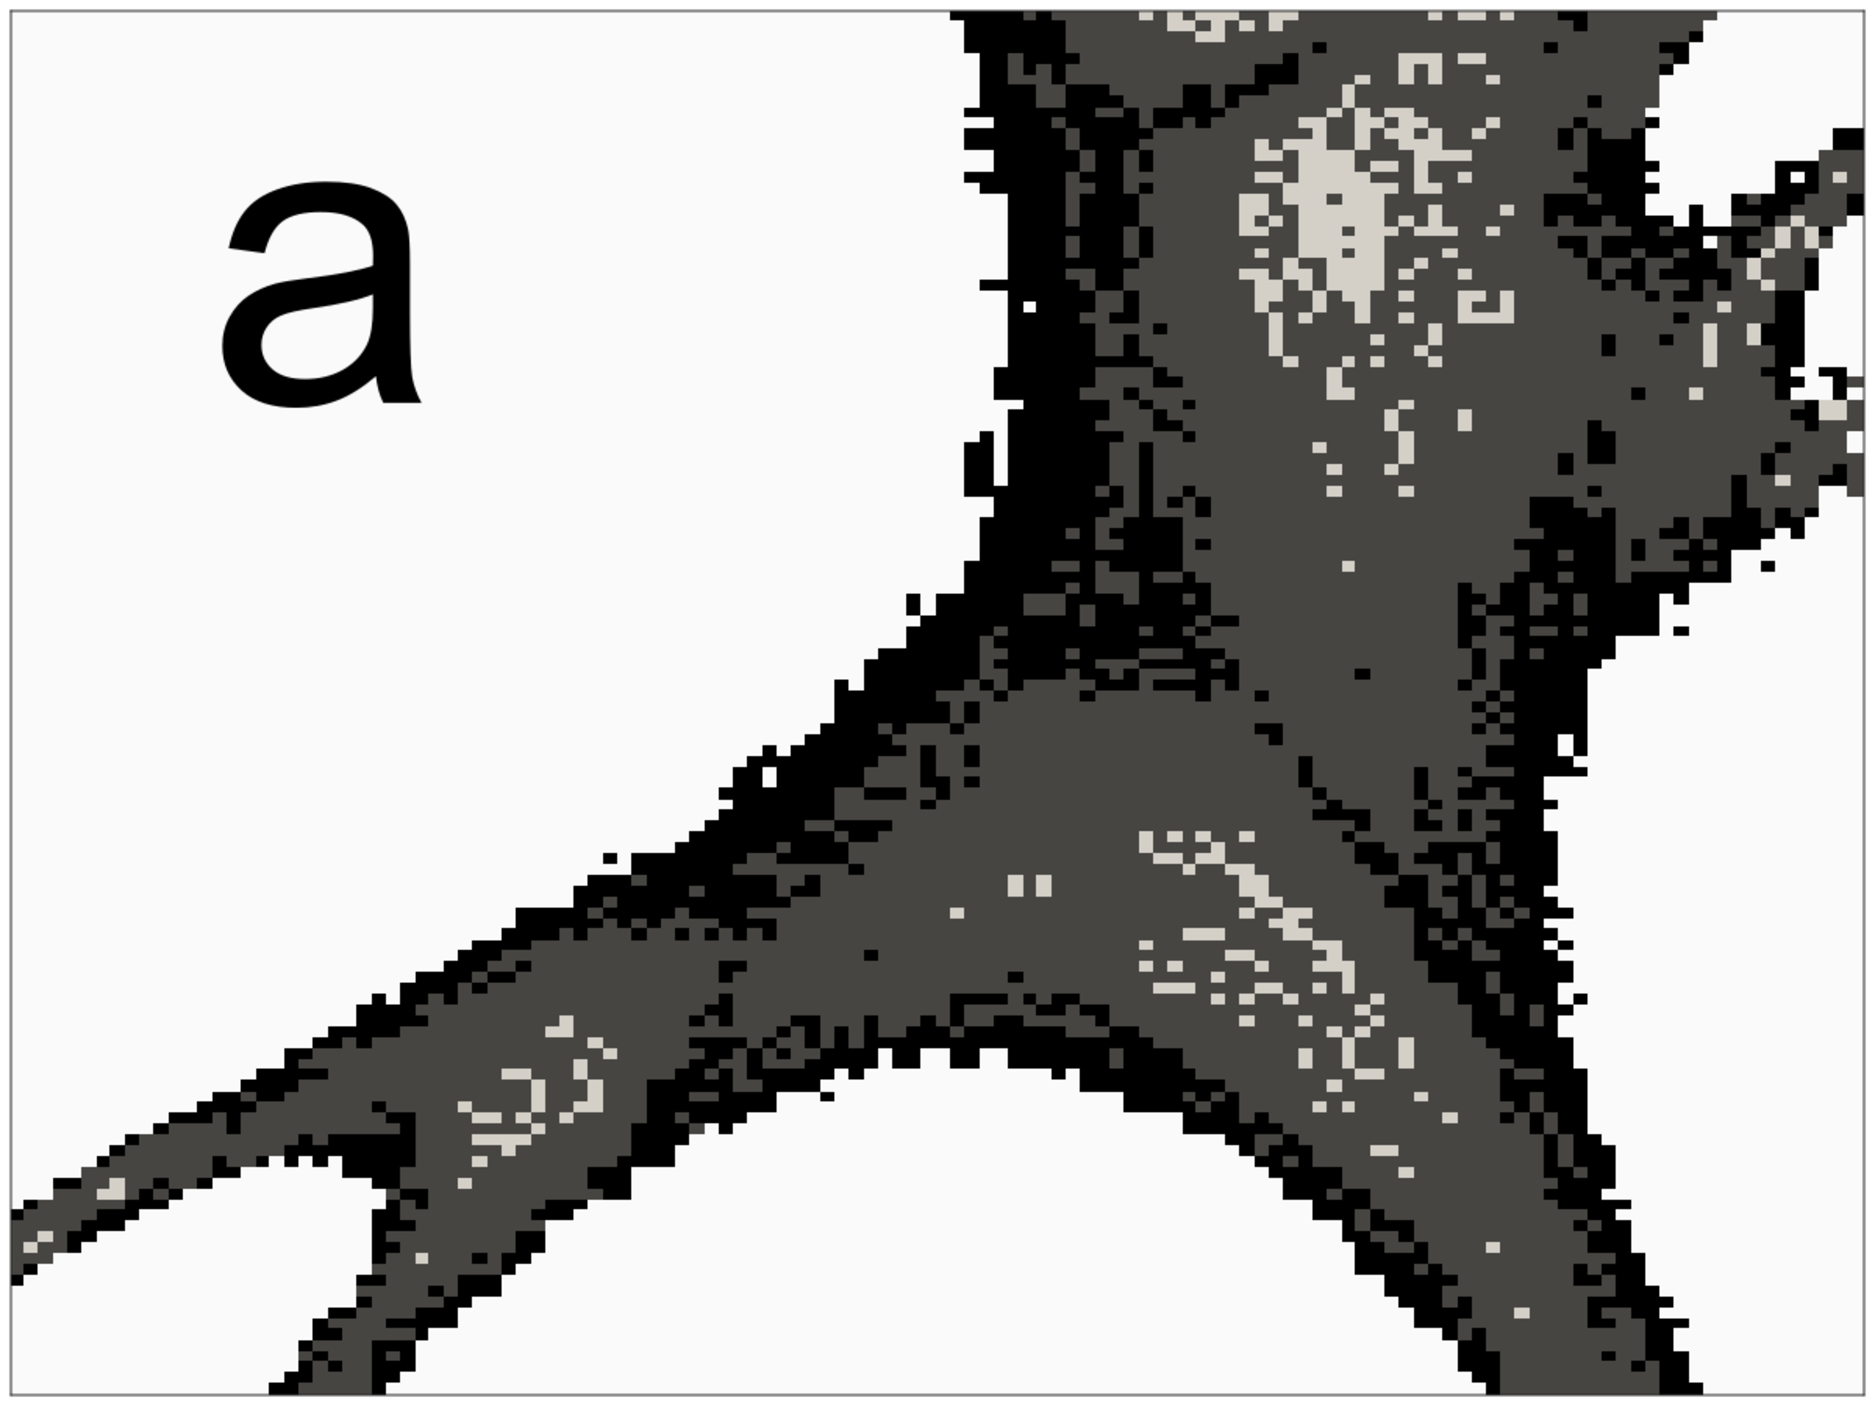
\includegraphics[width=0.35\textwidth]{m5_lu}
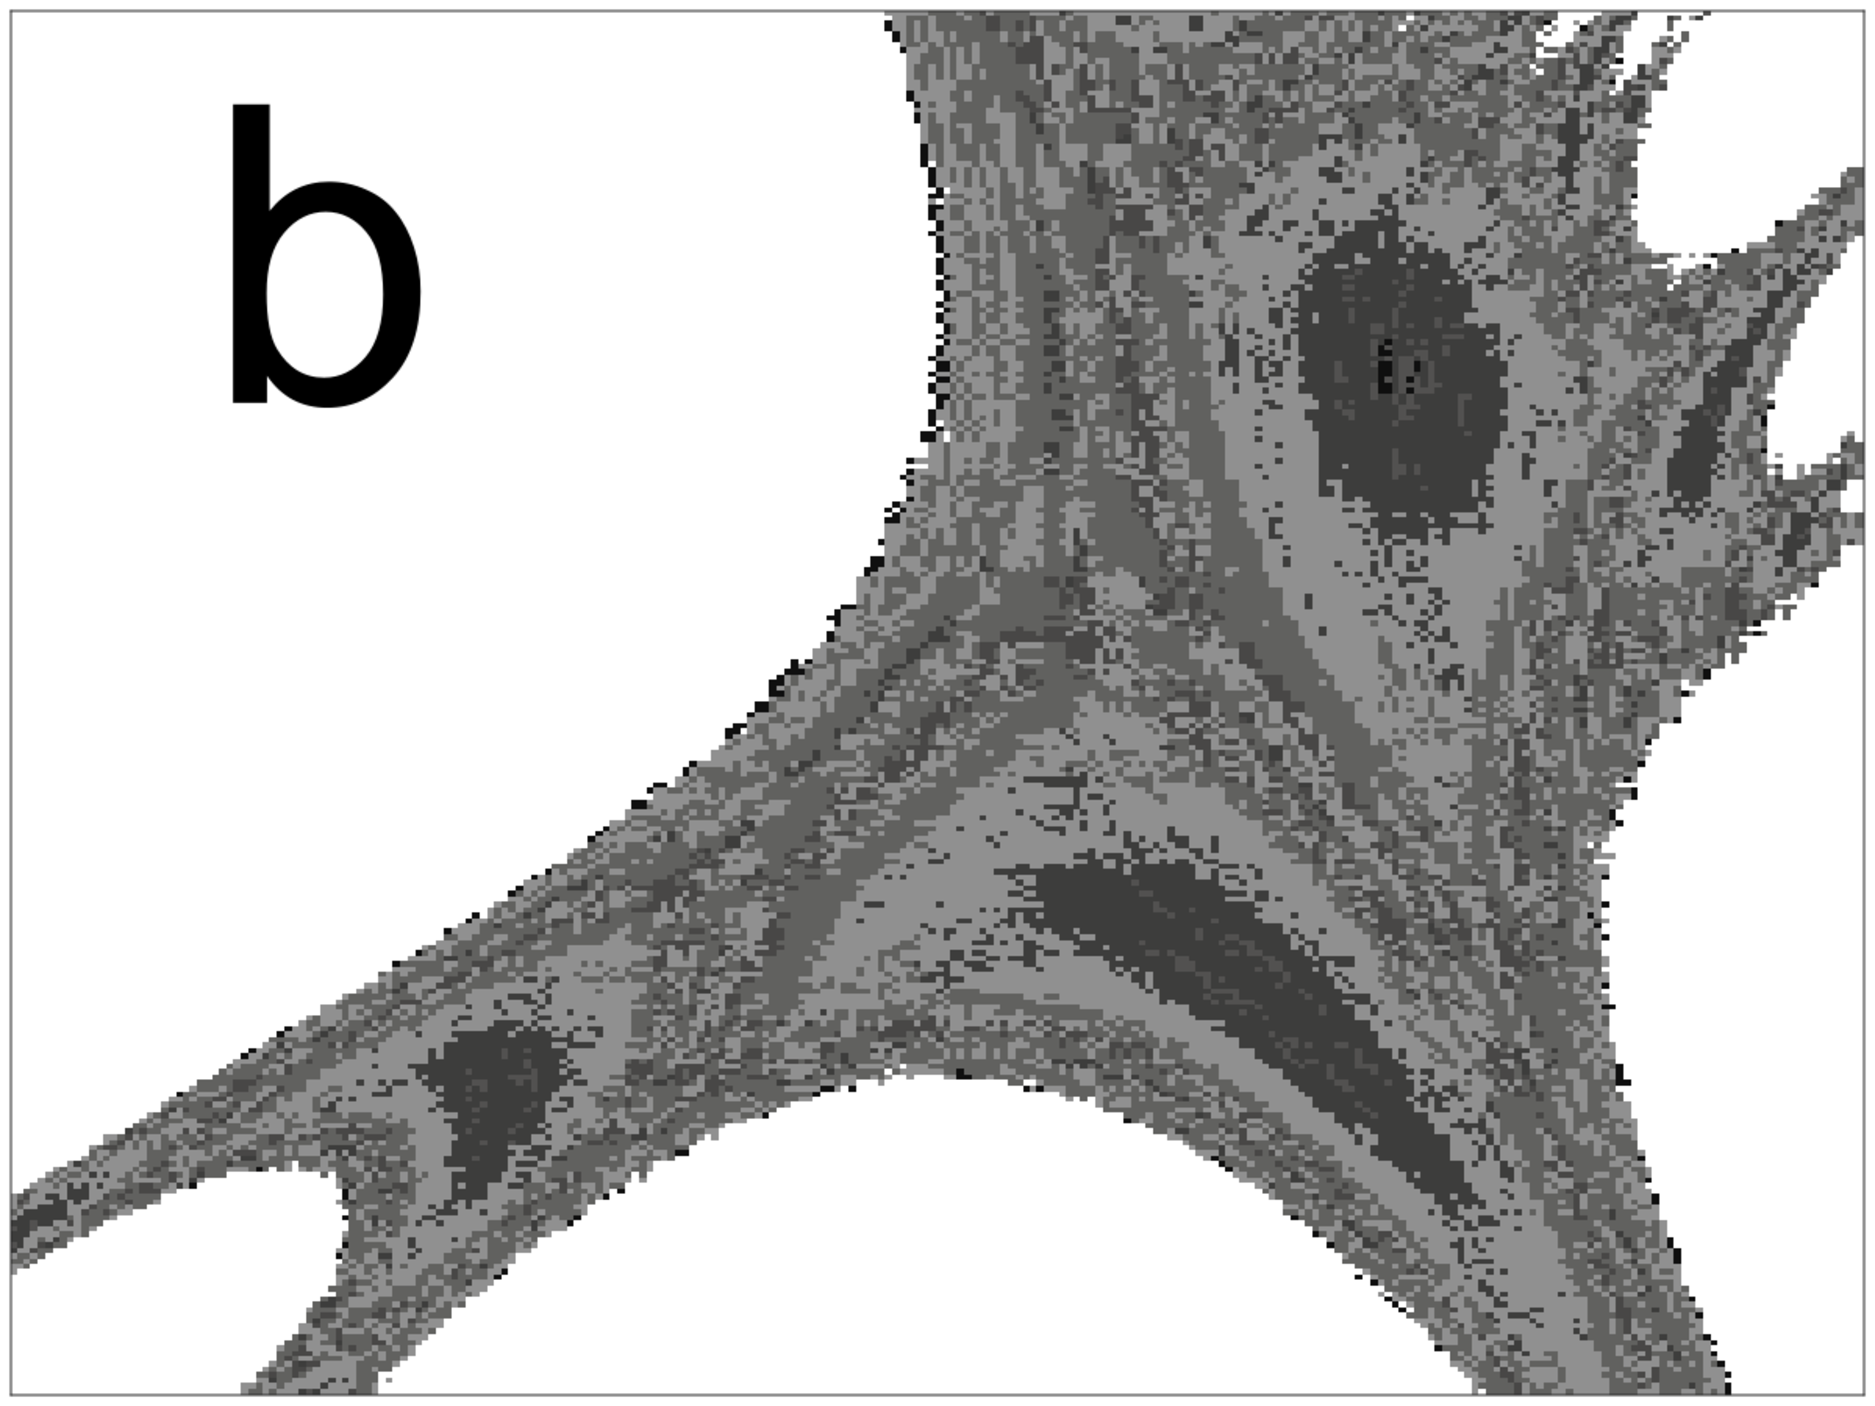
\includegraphics[width=0.35\textwidth]{m6_lu}
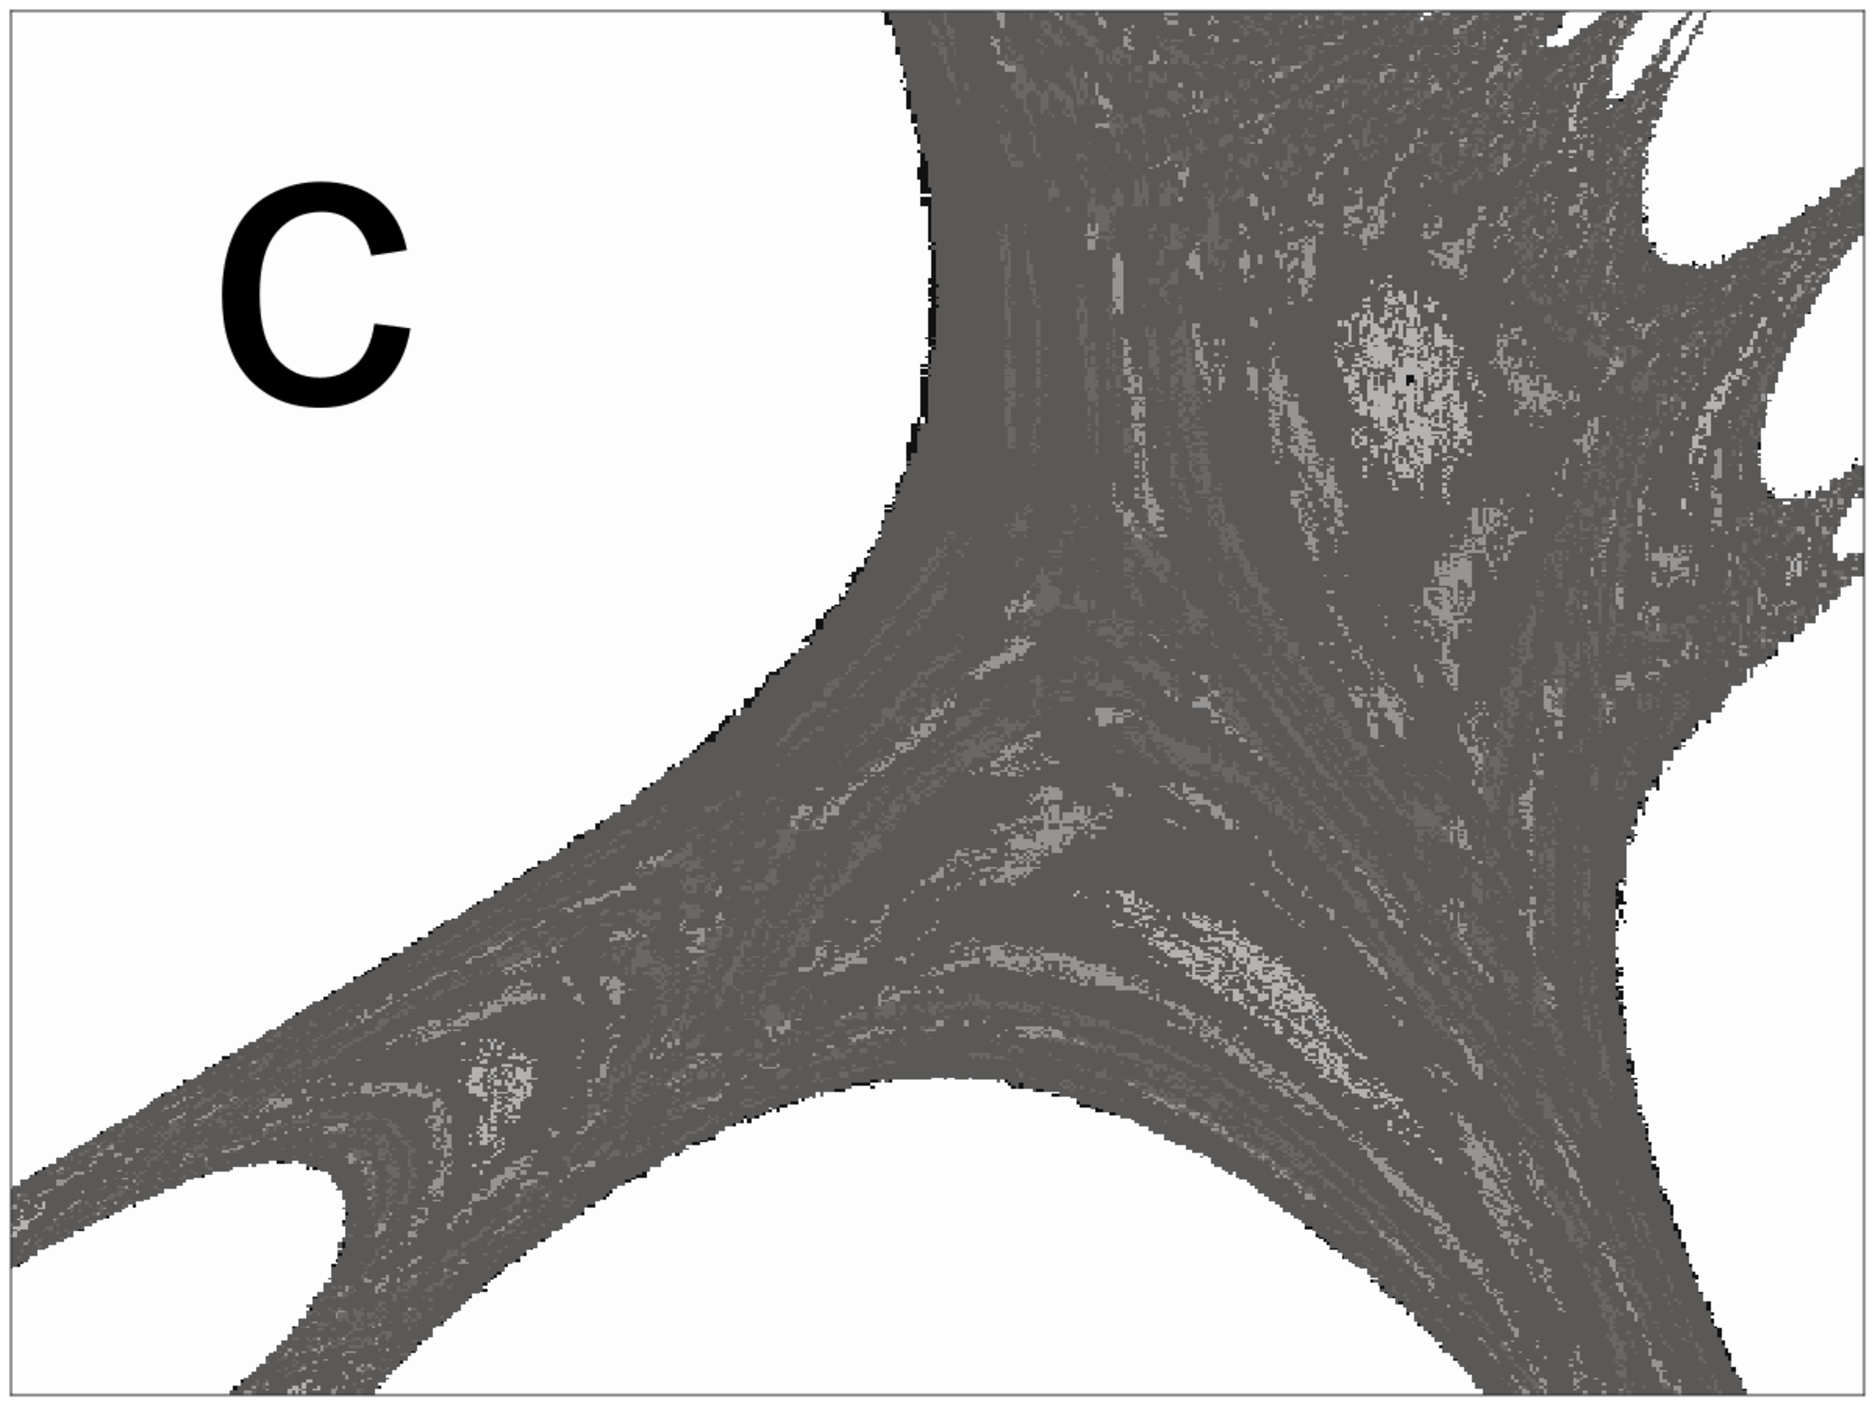
\includegraphics[width=0.35\textwidth]{m7_lu}\\
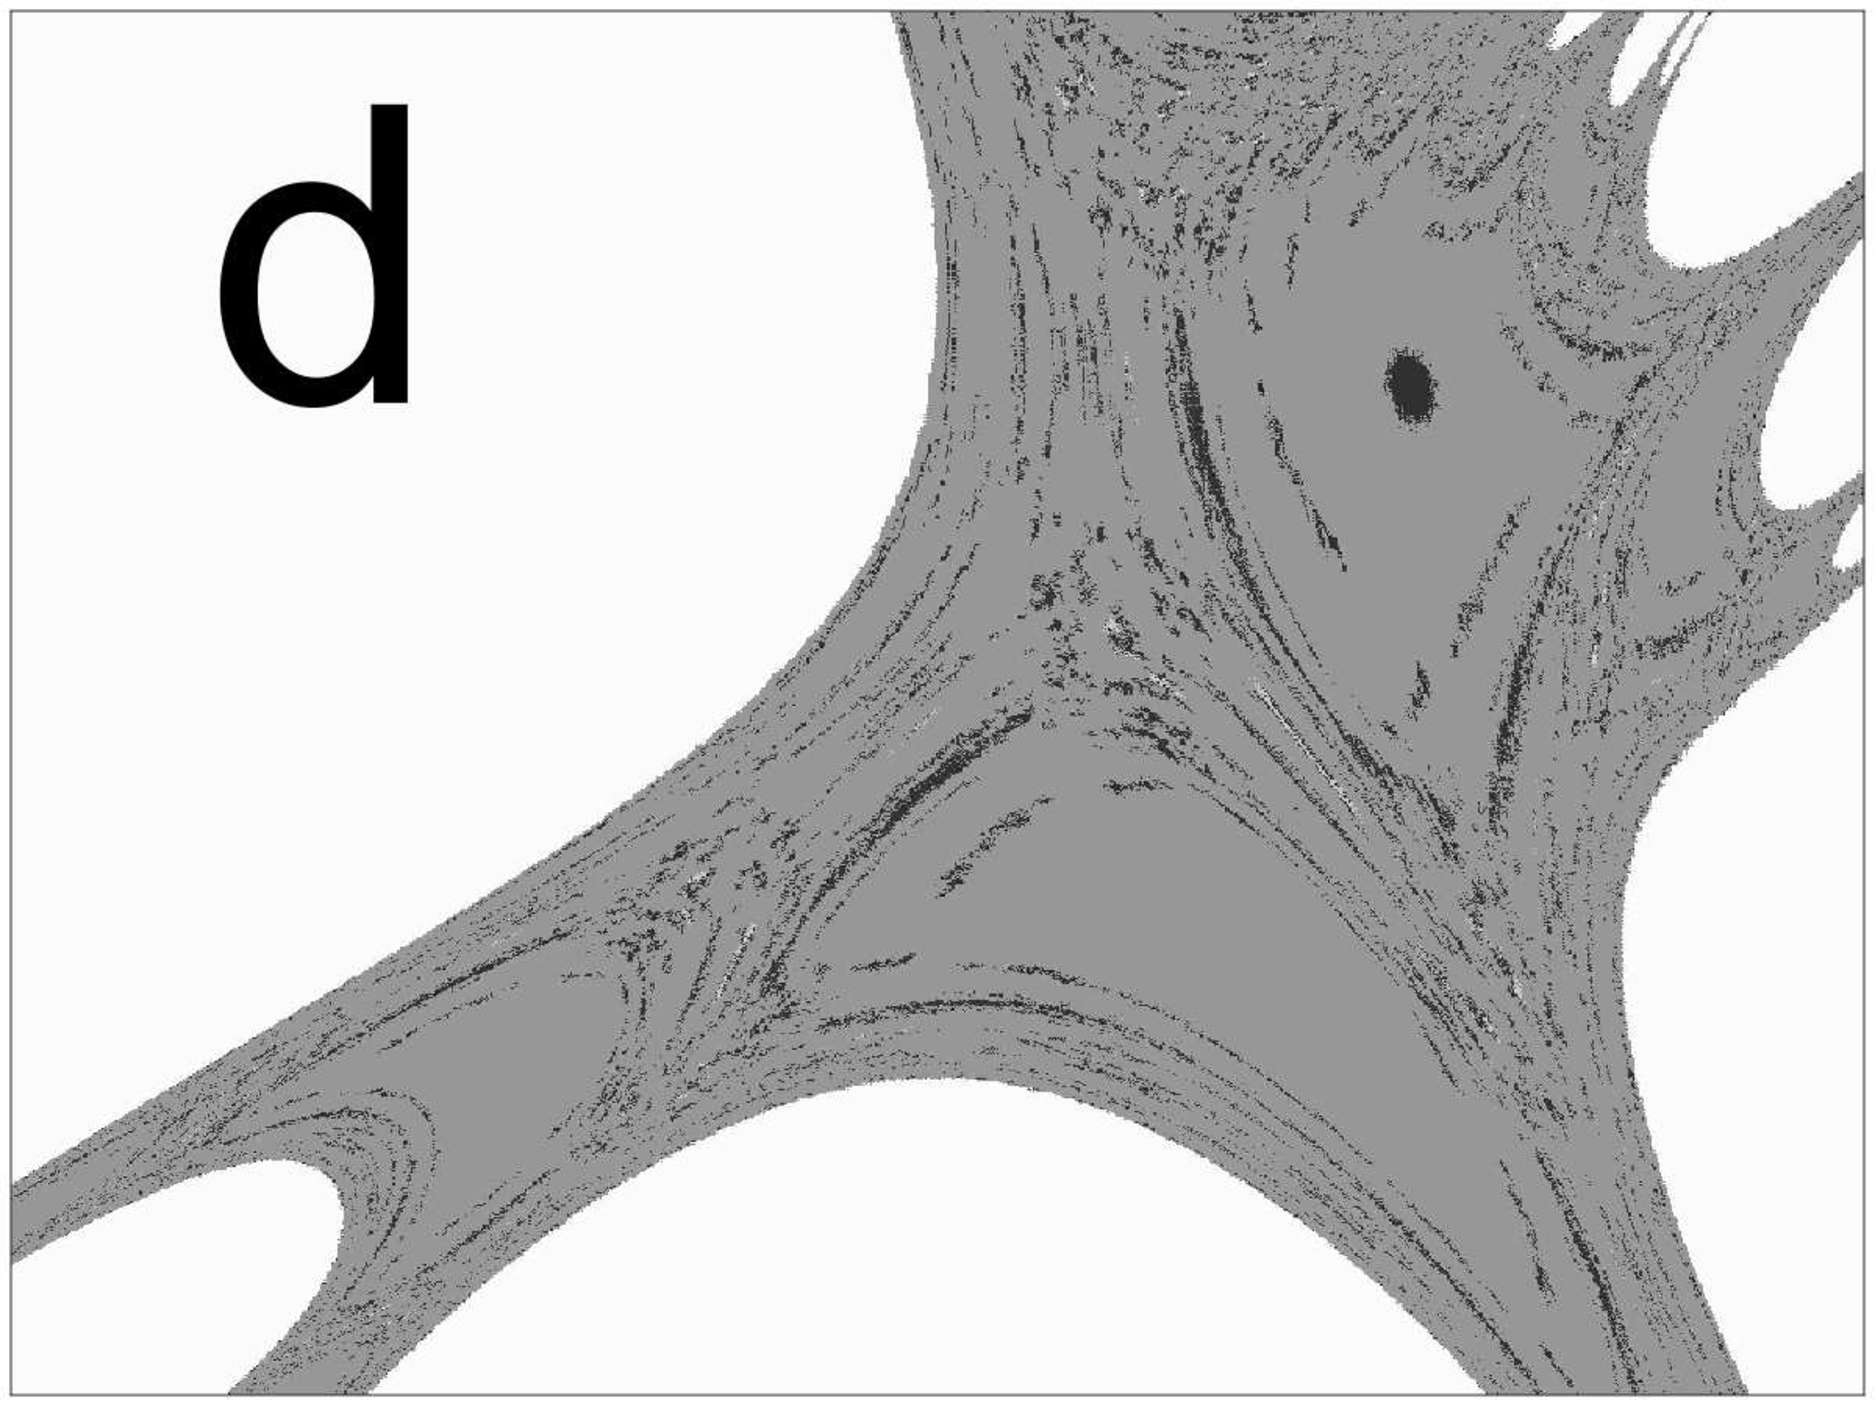
\includegraphics[width=0.35\textwidth]{m8_lu}
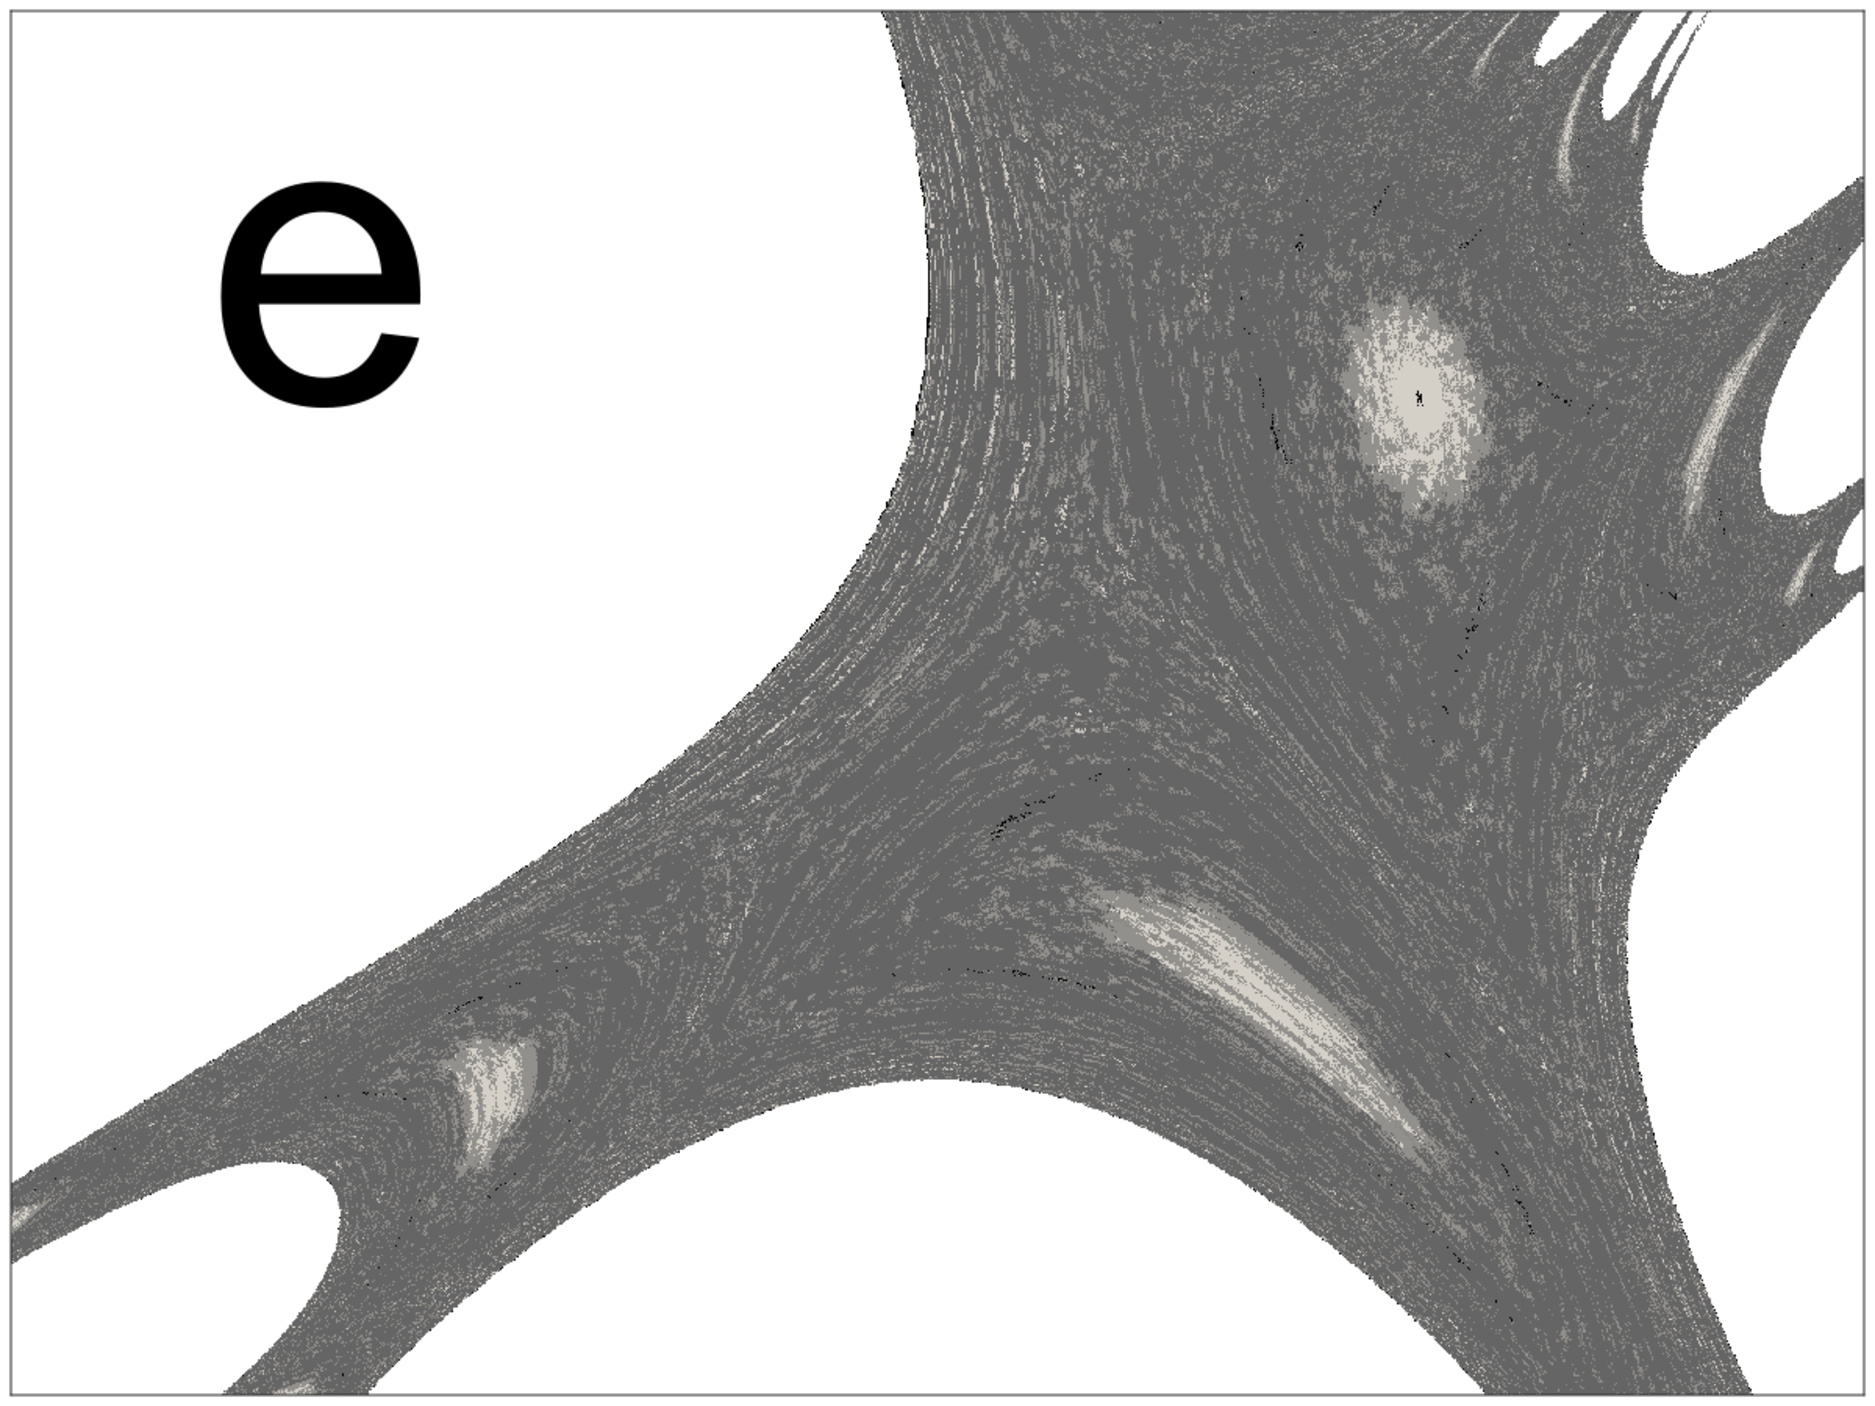
\includegraphics[width=0.35\textwidth]{m9_lu}
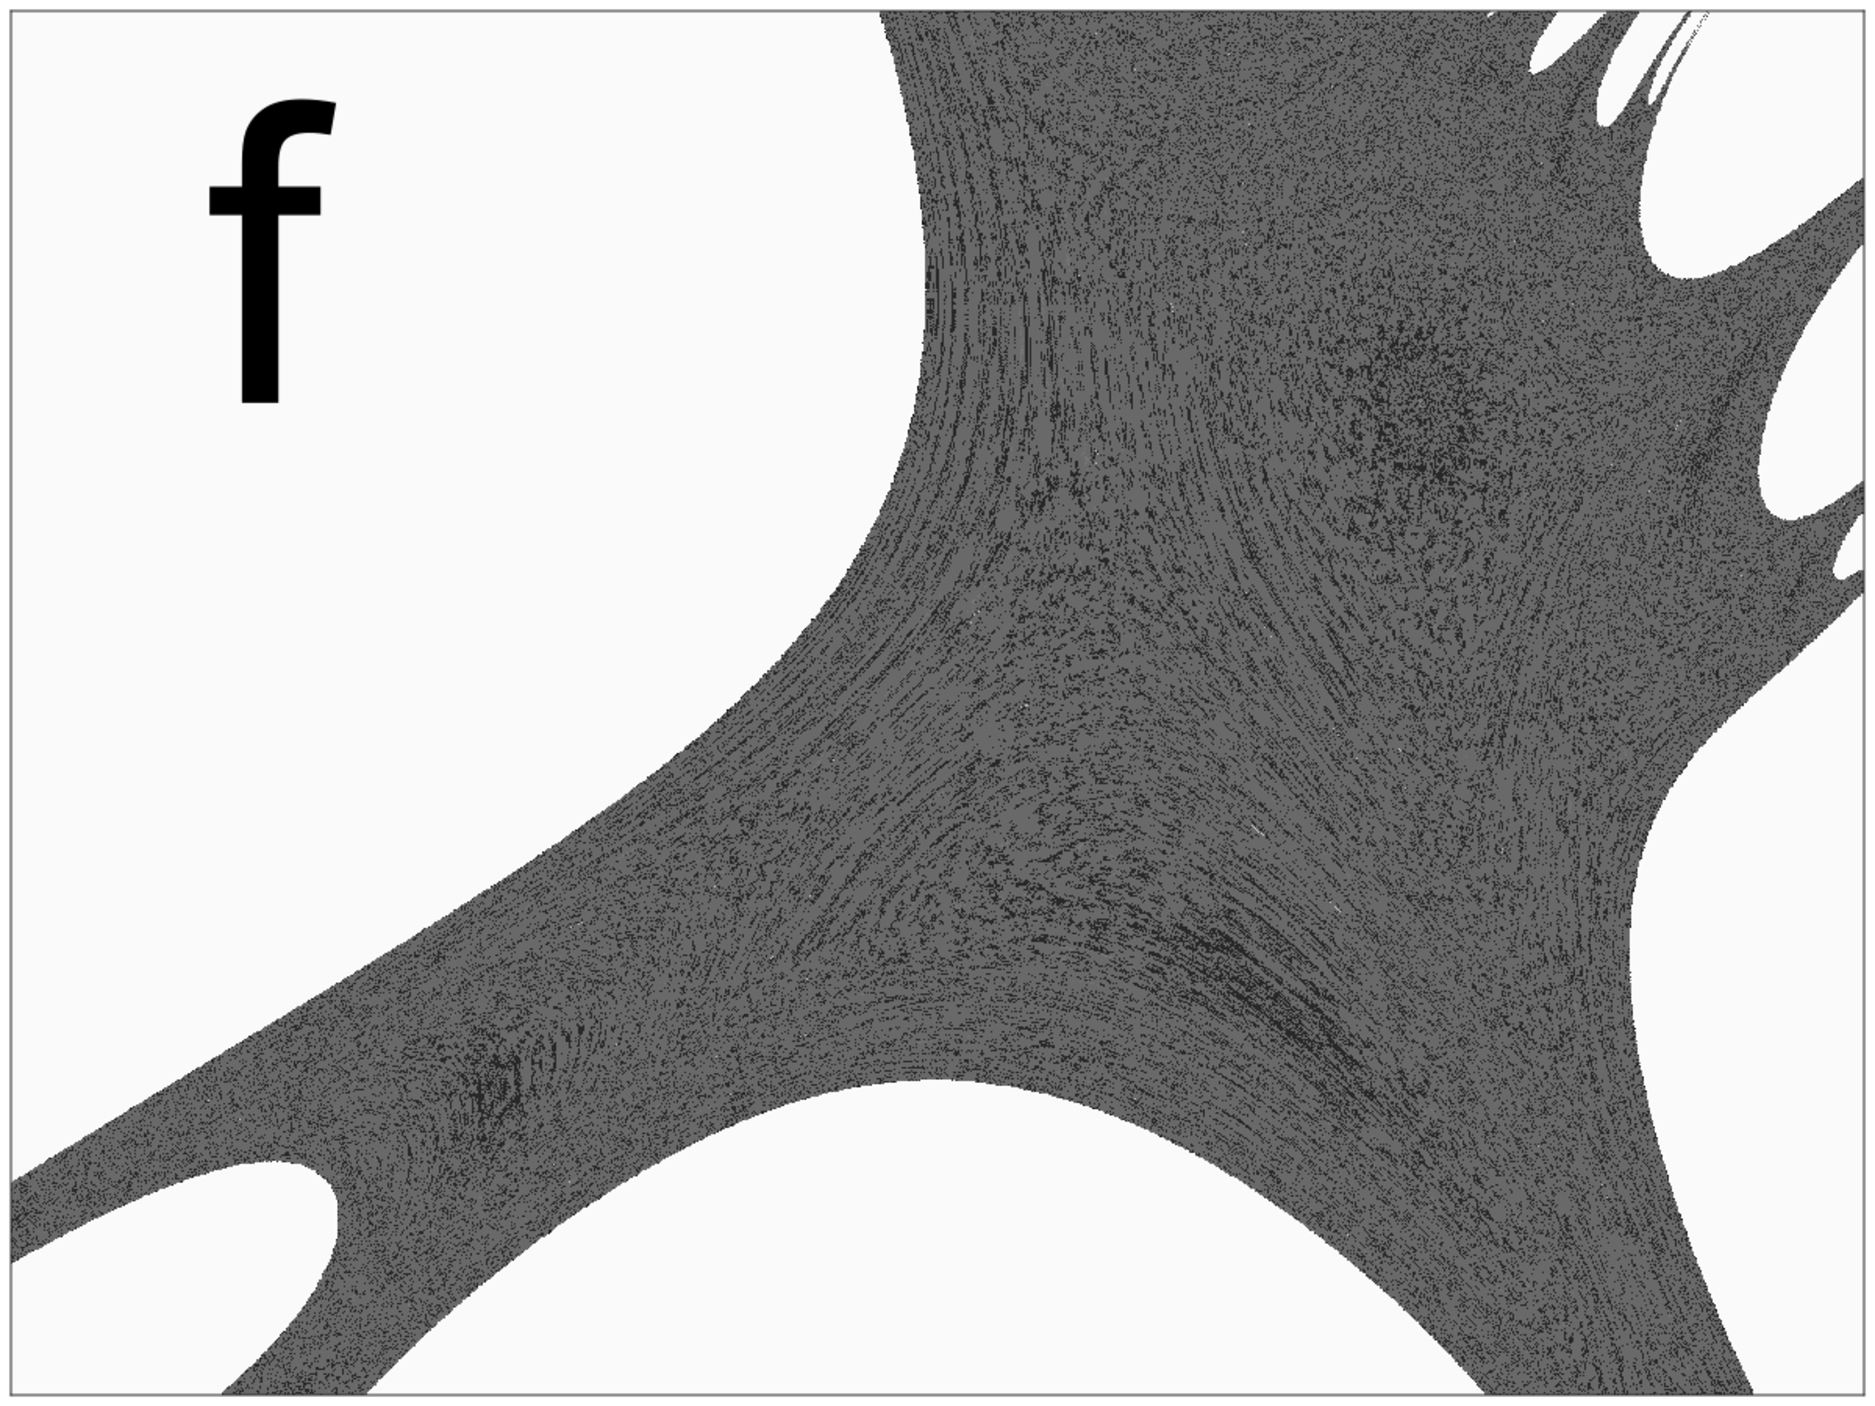
\includegraphics[width=0.35\textwidth]{m10_lu}\\
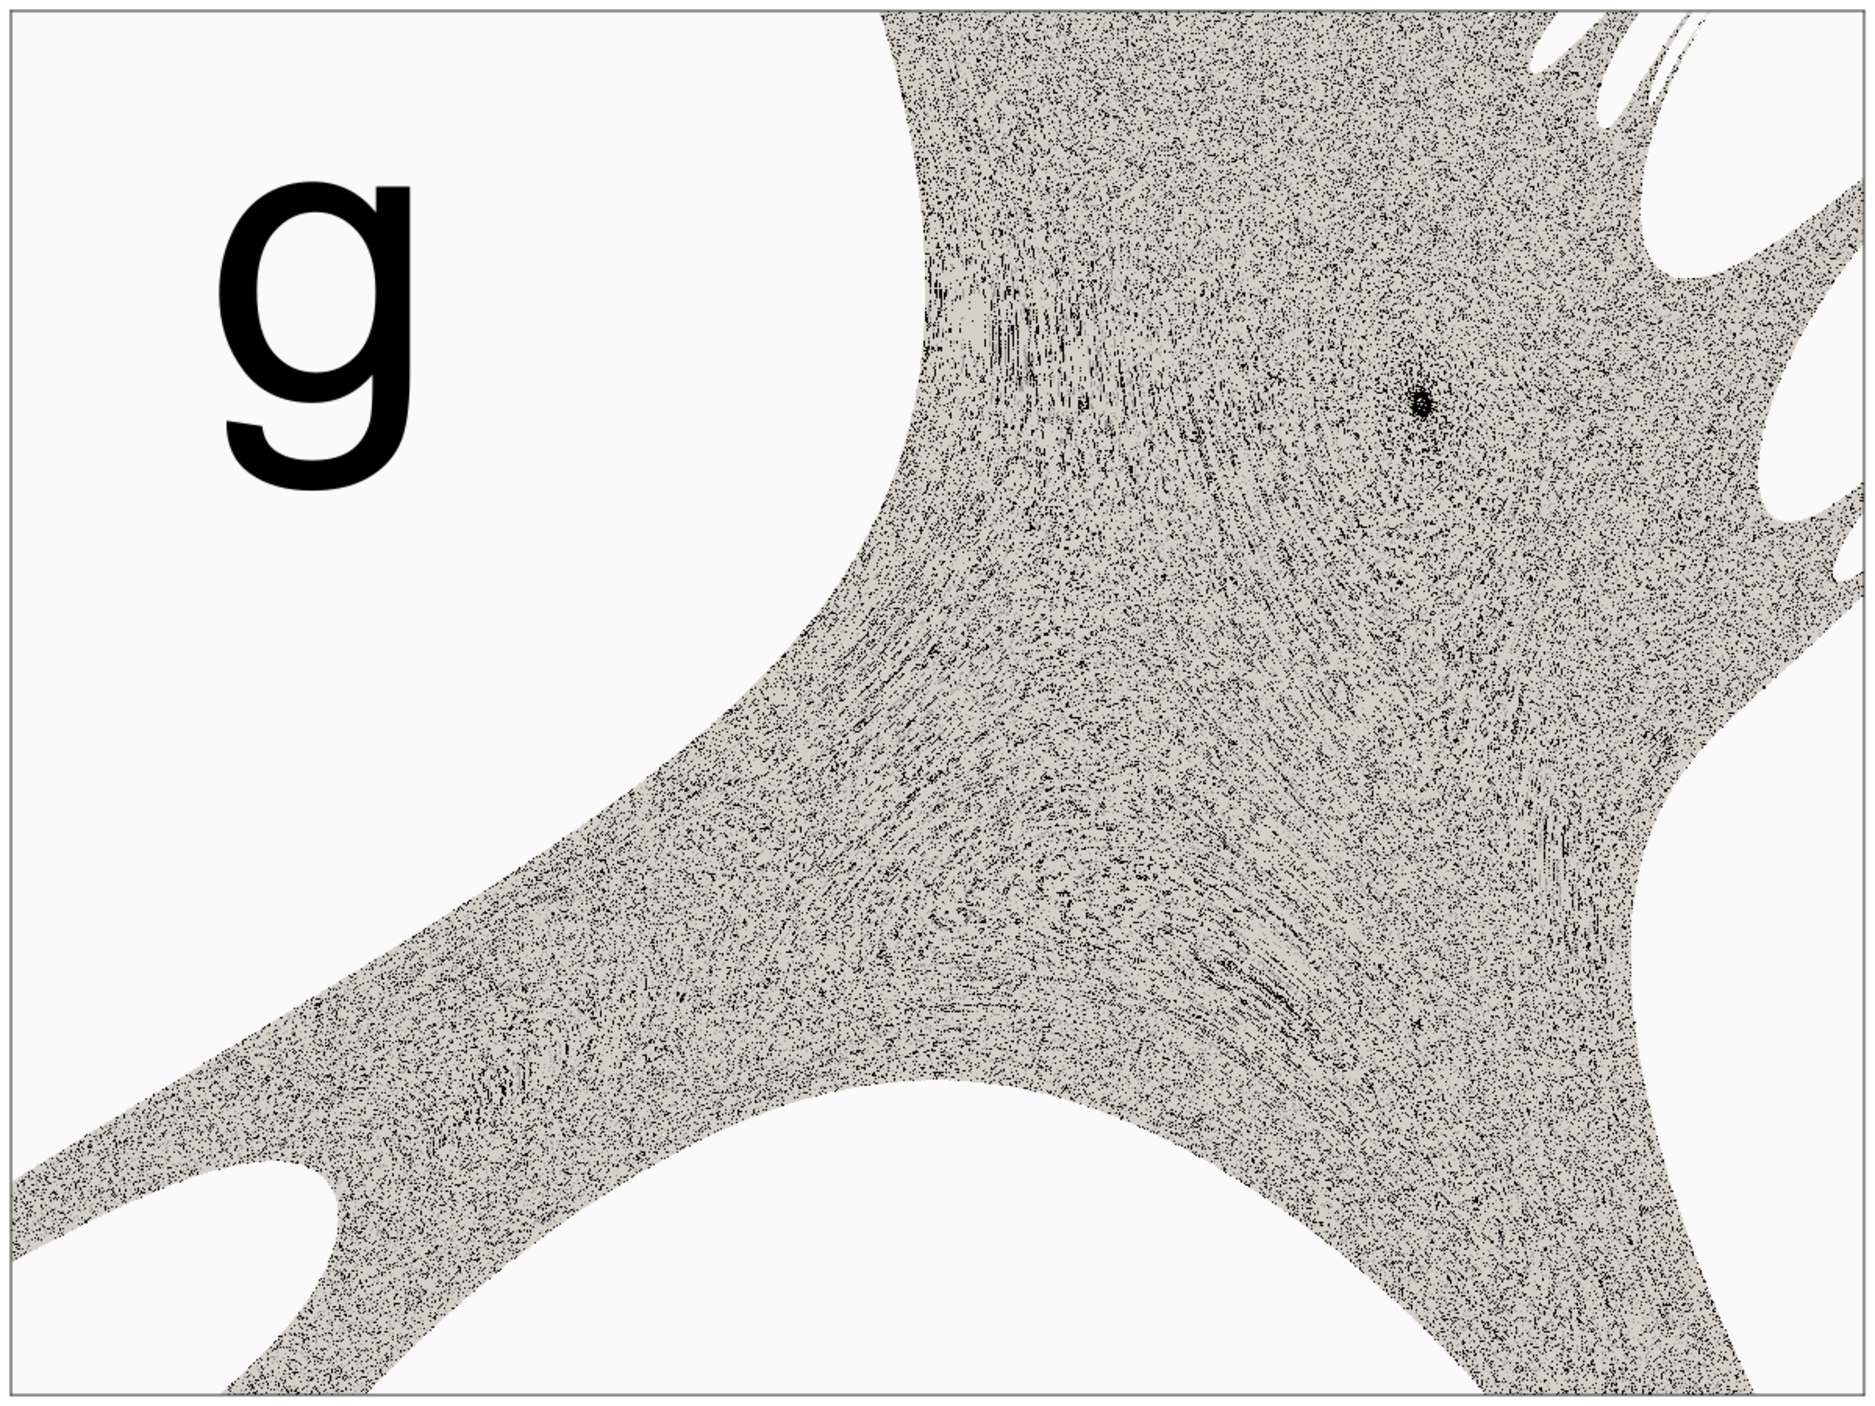
\includegraphics[width=0.35\textwidth]{m11_lu}
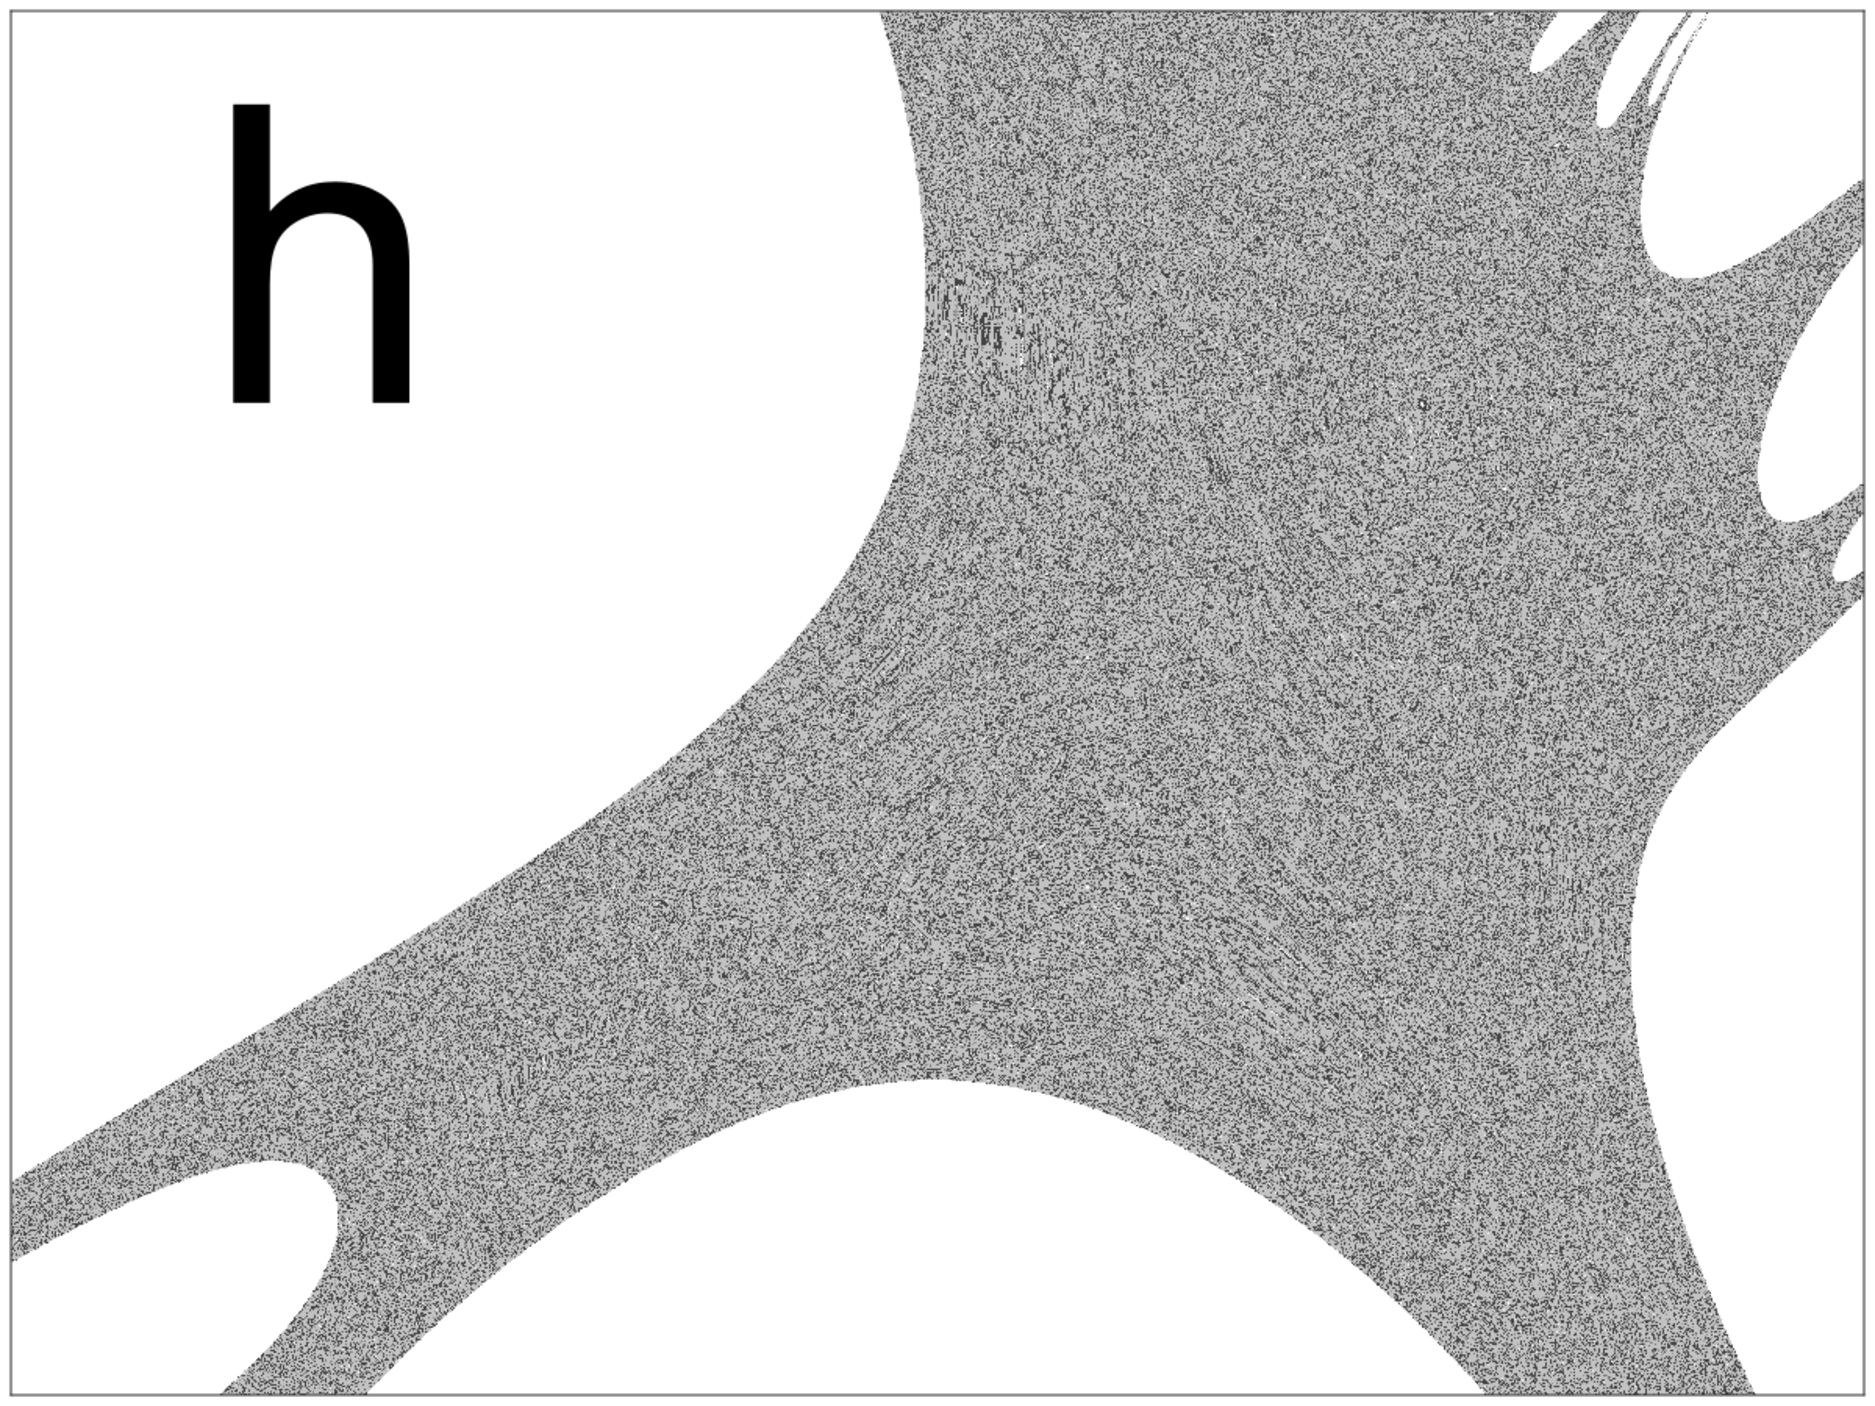
\includegraphics[width=0.35\textwidth]{m12_lu}
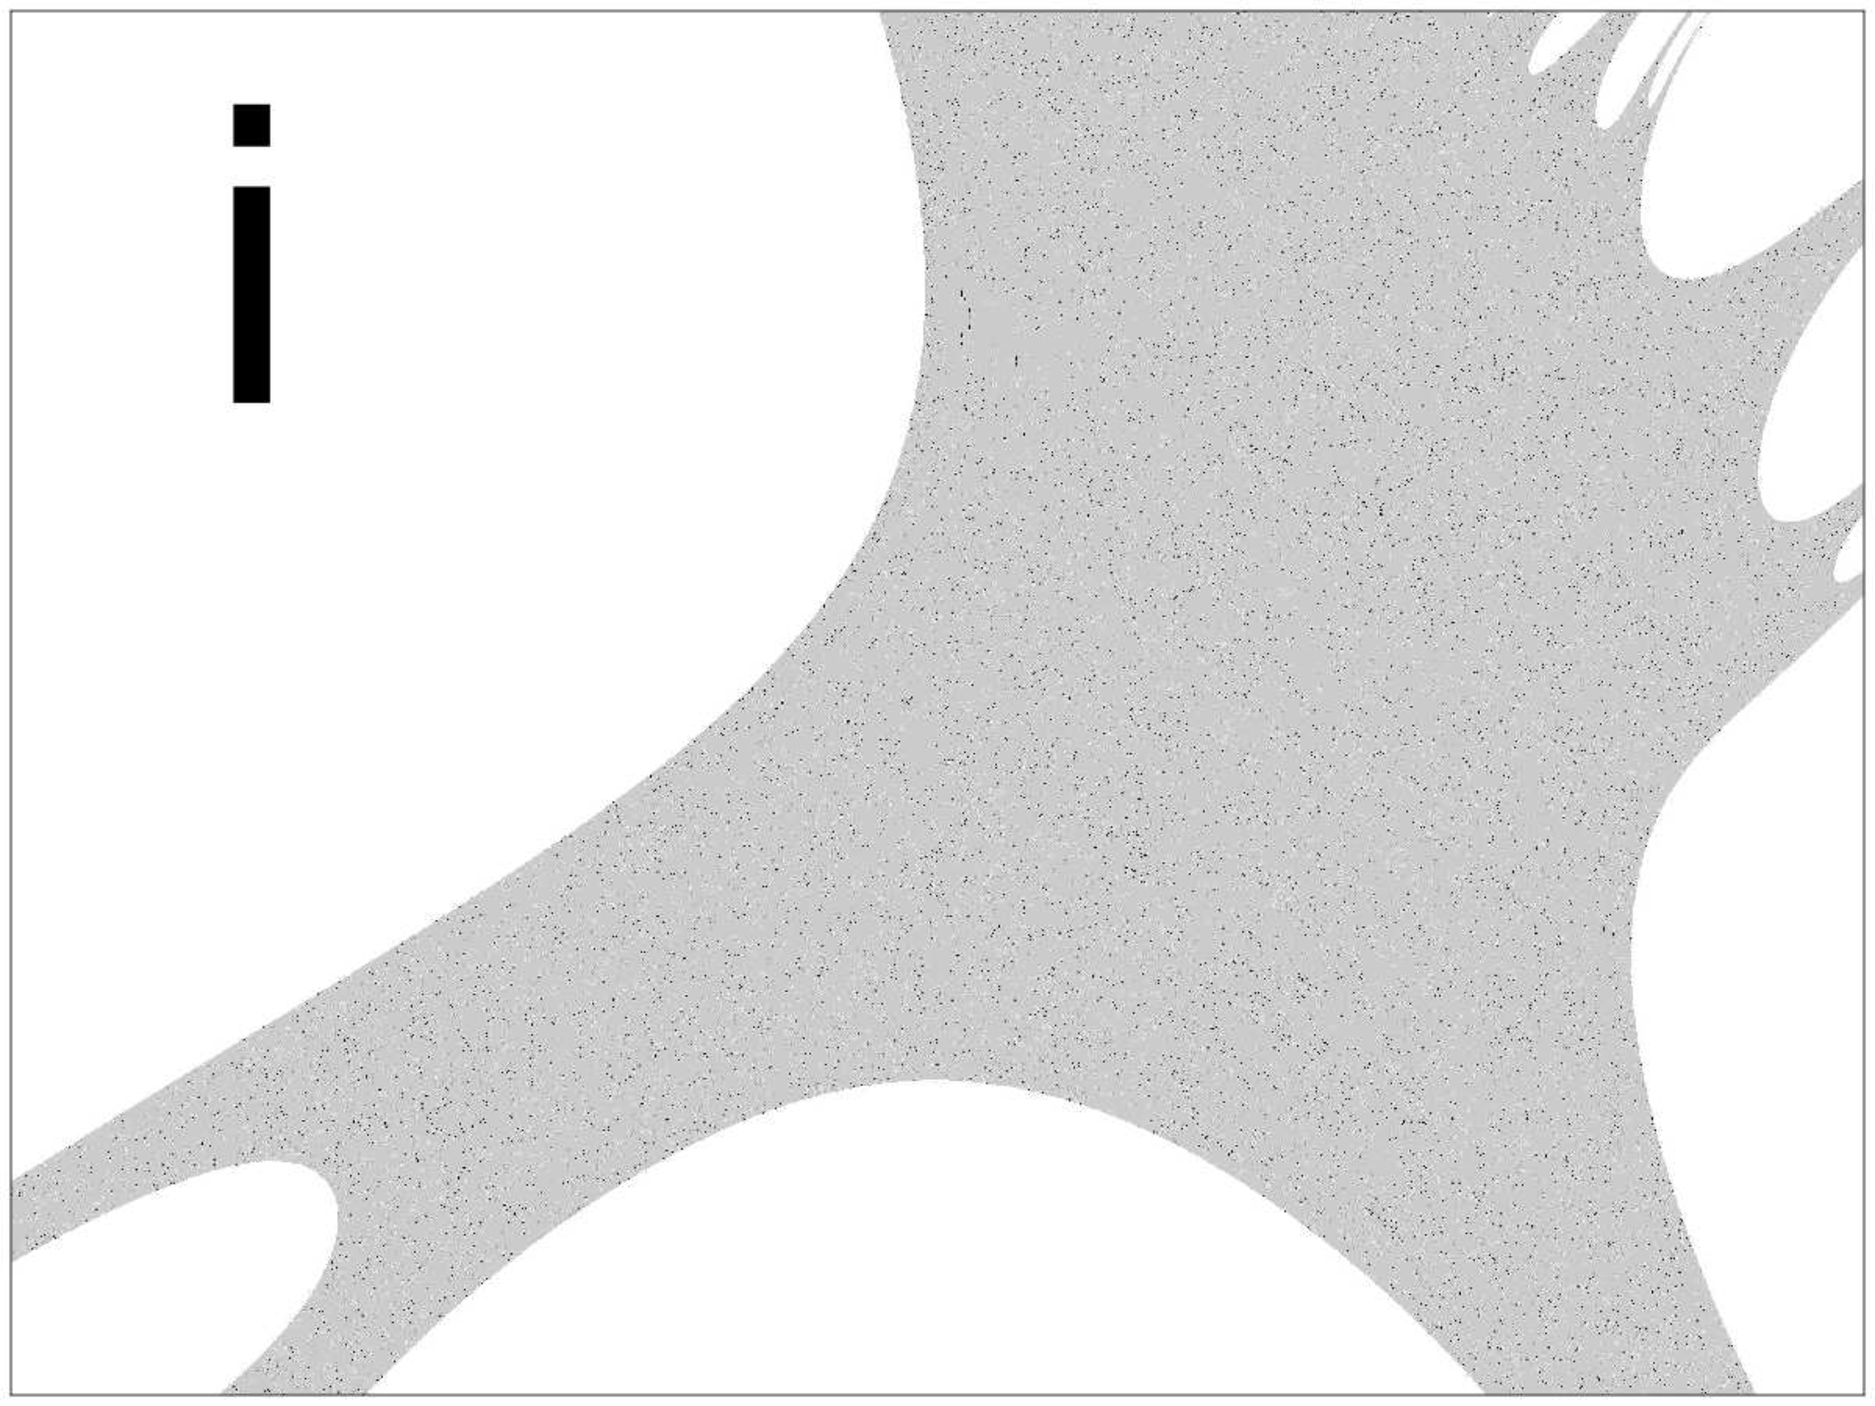
\includegraphics[width=0.35\textwidth]{m13_lu}\\
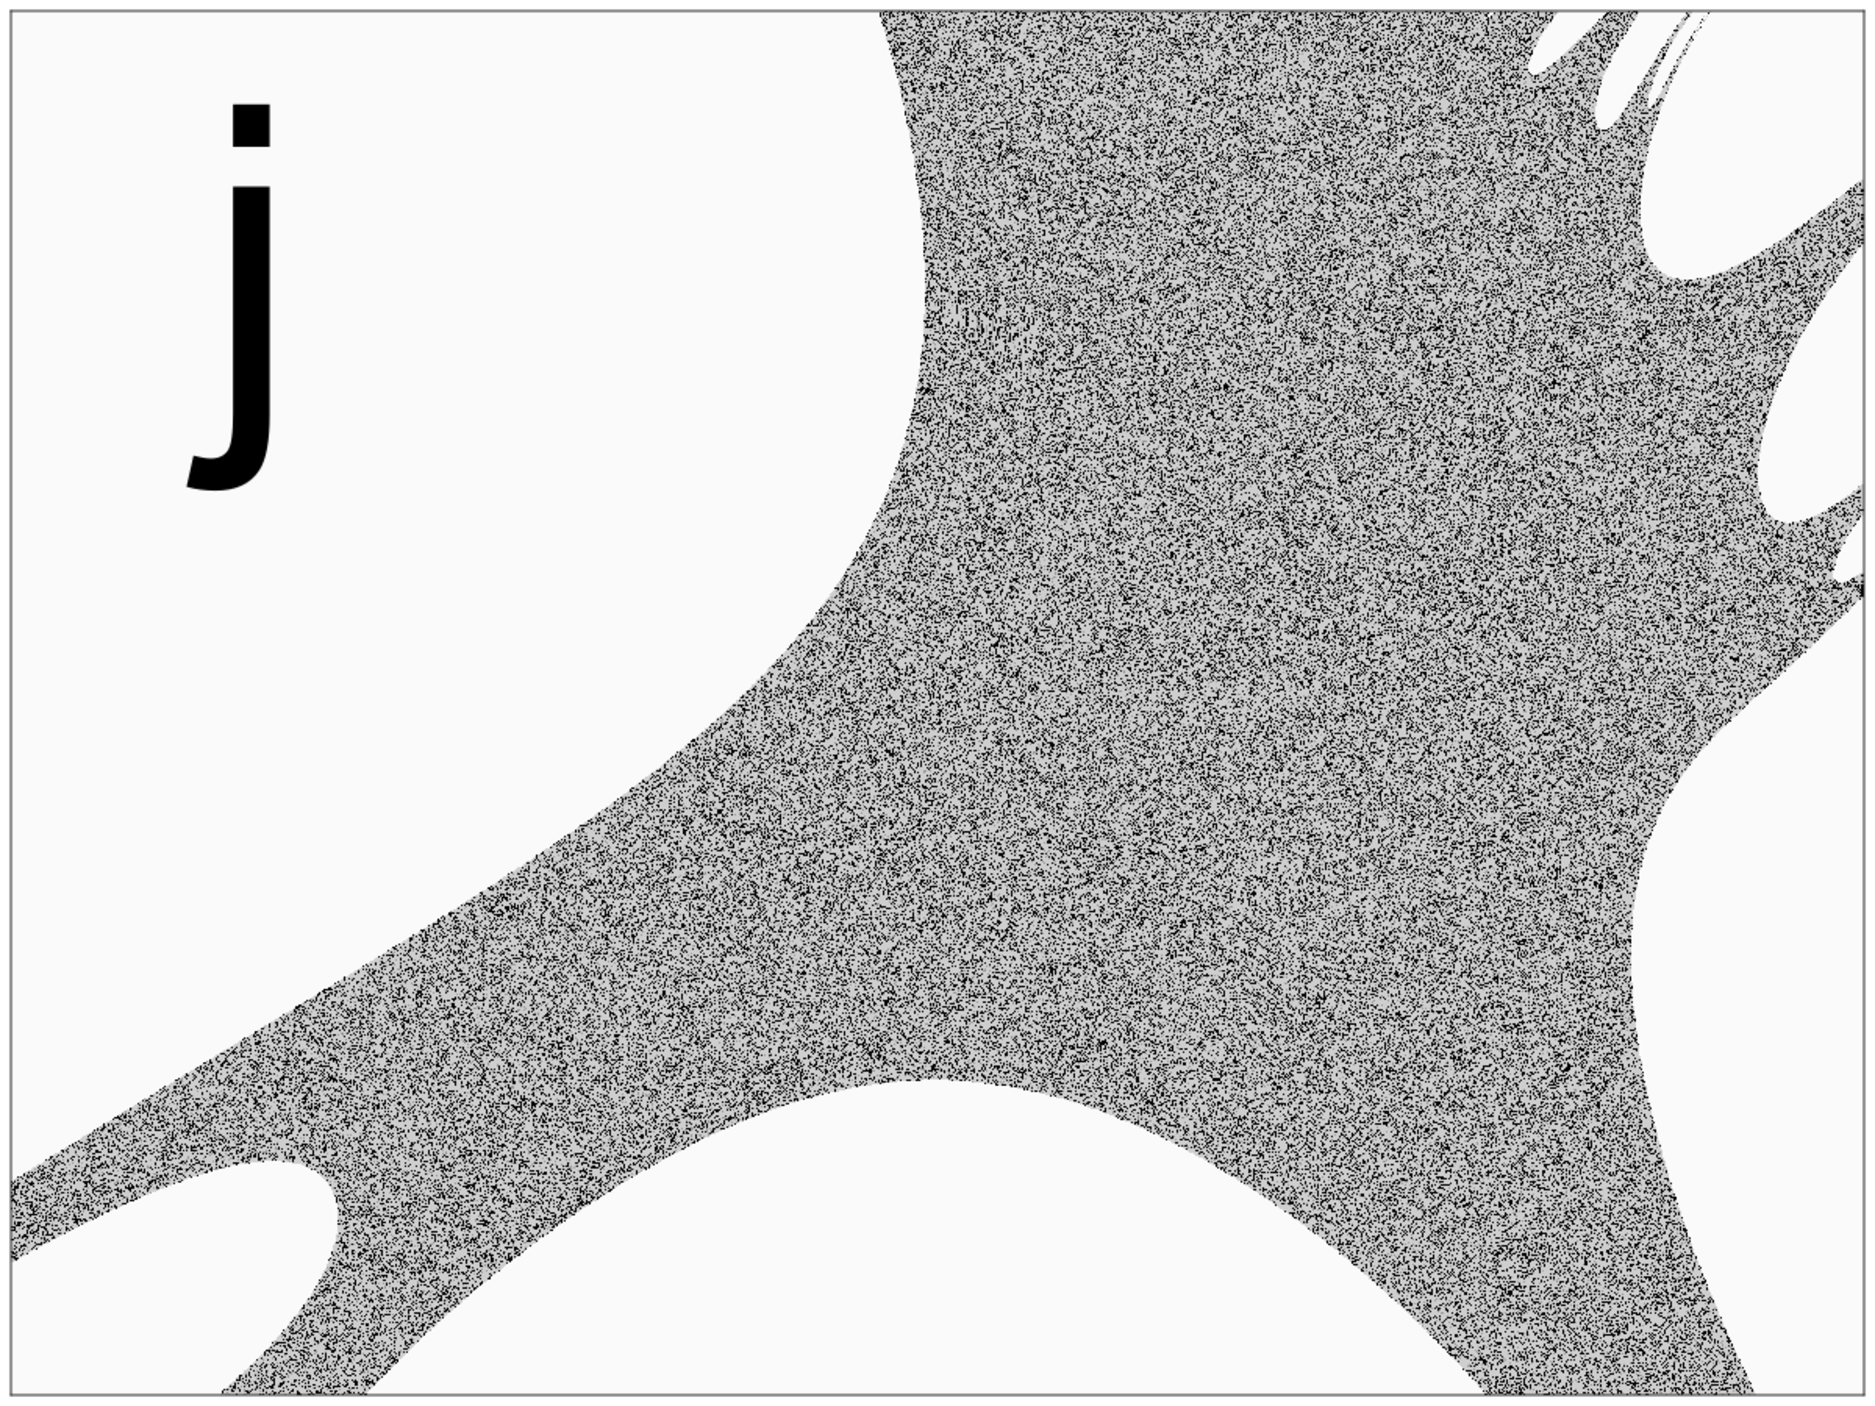
\includegraphics[width=0.35\textwidth]{m14_lu}
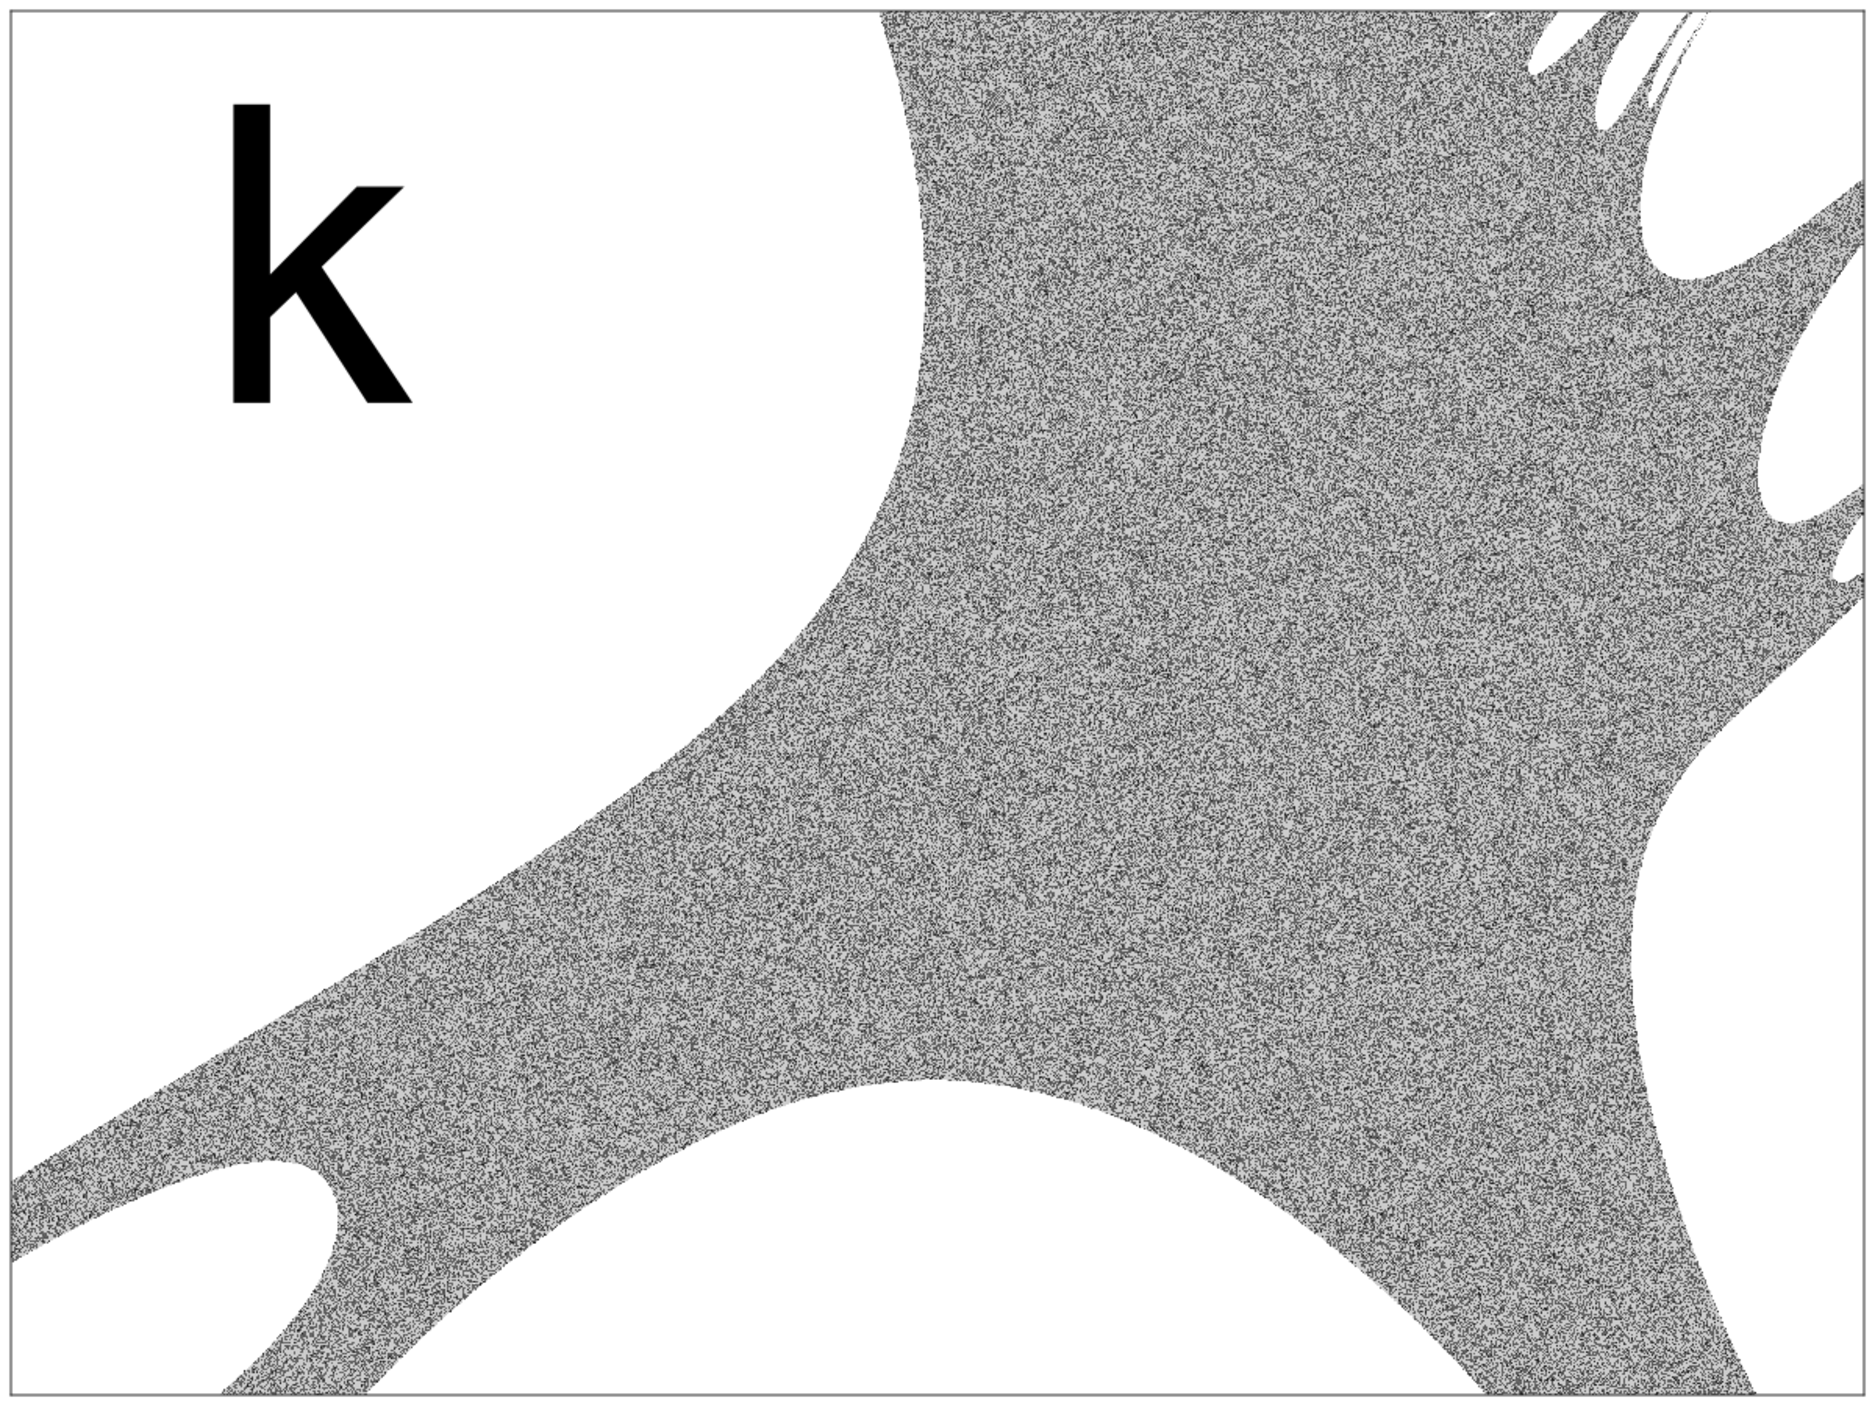
\includegraphics[width=0.35\textwidth]{m17_lu}
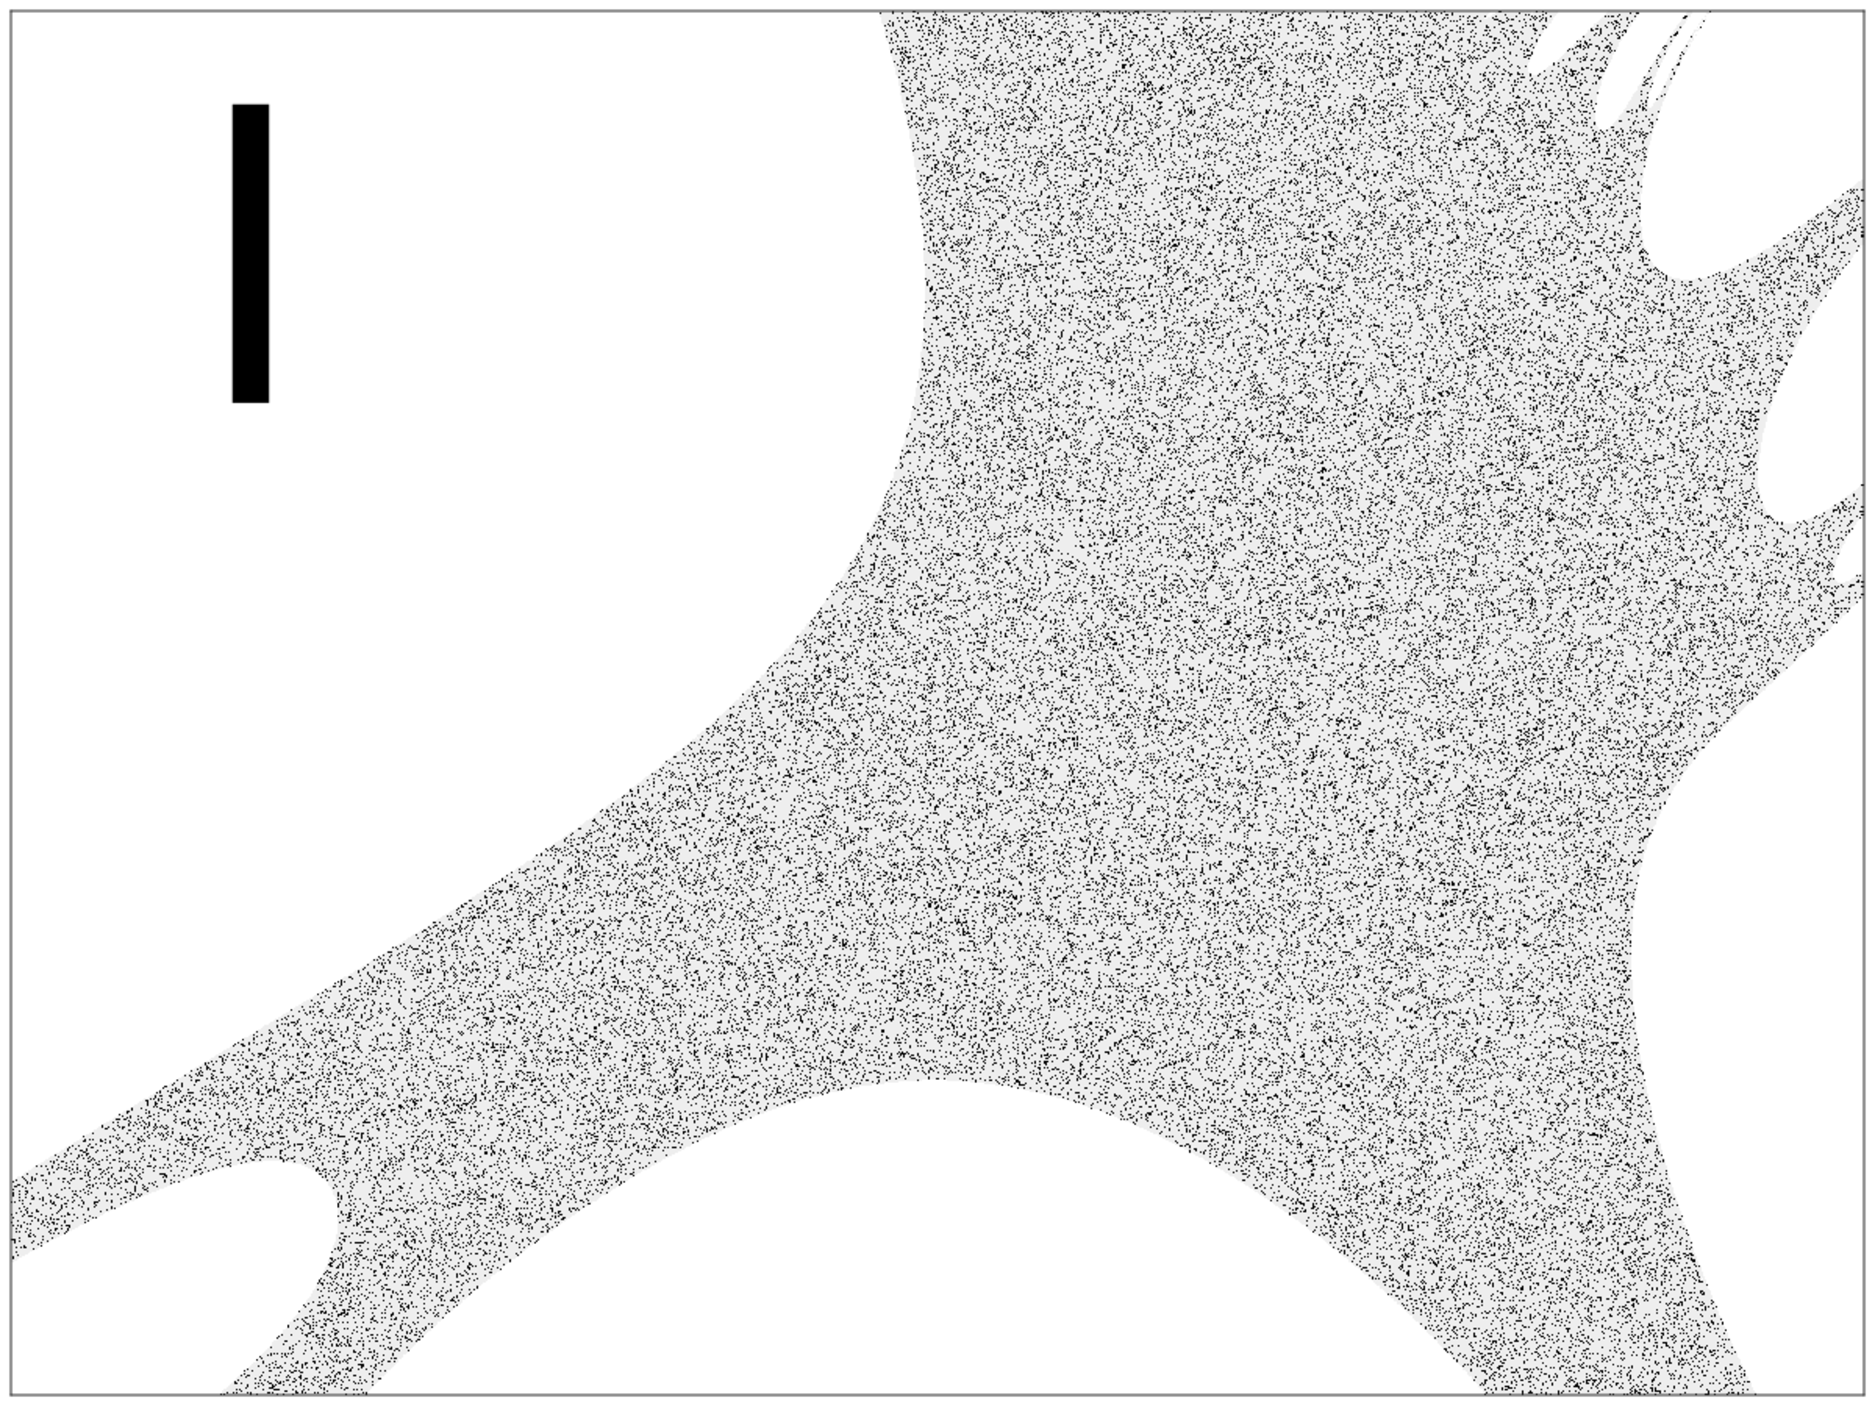
\includegraphics[width=0.35\textwidth]{m18_lu}\\
\end{tabular}
\caption{Áreas coexistentes en el dominio de atracción para: (a) $n_f=5$, (b) $n_f=6$, (c) $n_f=7$, (d) $n_f=8$, (e) $n_f=9$, (f) $n_f=10$, (g) $n_f=11$, (h) $n_f=12$, (i) $n_f=13$, (j) $n_f=14$, (k) $n_f=17$, (l) $n_f=18$.}
\label{fig:avvelo}
\end{figure*}

Con el fin de poder distinguir las diferentes áreas coexistentes, se ha utilizado una amplia gama de tonos grises en cada figura.
Se debe tener en cuenta que cada figura tiene su propio rango de grises, esto significa que, por ejemplo, un área casi blanca cuando $n_f = 5$ (Fig. \ref{fig:avvelo} .a) corresponde a un período de $6$, mientras que un área más oscura en una figura con mayor $n_f$ puede corresponder a un período superior a mil (Fig. \ref{fig:avvelo} .e).
Estas cifras permiten reflejar los complejos dominios de atracción que aparecen al digitalizar.

Se puede ver en la Fig. \ref{fig:avvelo} cuanto menor es el valor de $n_f$, mayor es el área de ICs que tiende a divergir y converger a puntos fijos.
A medida que $n_f$ aumenta, el área de puntos divergentes y fijos disminuye.
Estas figuras junto con la tabla \ref{tabla} permiten interpretar fácilmente el comportamiento del sistema.
En la tabla \ref{tabla} las longitudes de las secuencias que aparecen en el dominio de atracción para cada $n_f$ se ordenan por el número de circuitos integrados menos numerosos que convergen en ese ciclo.
Se puede ver la tasa de ocurrencia.
De hecho, las figuras con valores más bajos de $n_f$ presentan superficies irregulares o rugosas, señalando que los ciclos de diferentes longitudes coexisten allí.
Por ejemplo, para $n_f = 5$ hay una prevalencia de ciclos de períodos cortos.
En ese caso, existen solo dos ciclos límite, la zona gris más clara corresponde al dominio de atracción de los ciclos límite de longitud seis, que es el ciclo menos numeroso, de acuerdo con la Tabla \ref{tabla}, y la zona más oscura corresponde al dominio de atracción de longitud de ciclo dos.

Aunque para $n_f \geqslant 13$ (Figuras \ref{fig:avvelo}.i a \ref{fig:avvelo}.l), el dominio de atracción parece ser suave y uniforme, todavía hay ciclos con diferentes períodos que coexisten en el atractor por $ n_f = 14 $, $ 17 $ y $ 18 $.
Esto se puede ver si ampliamos una sección de las figuras (Fig.\ref{fig:m_zoom}).
%
\begin{figure}
    \centering
    \begin{subfigure}[t]{0.49\textwidth}
        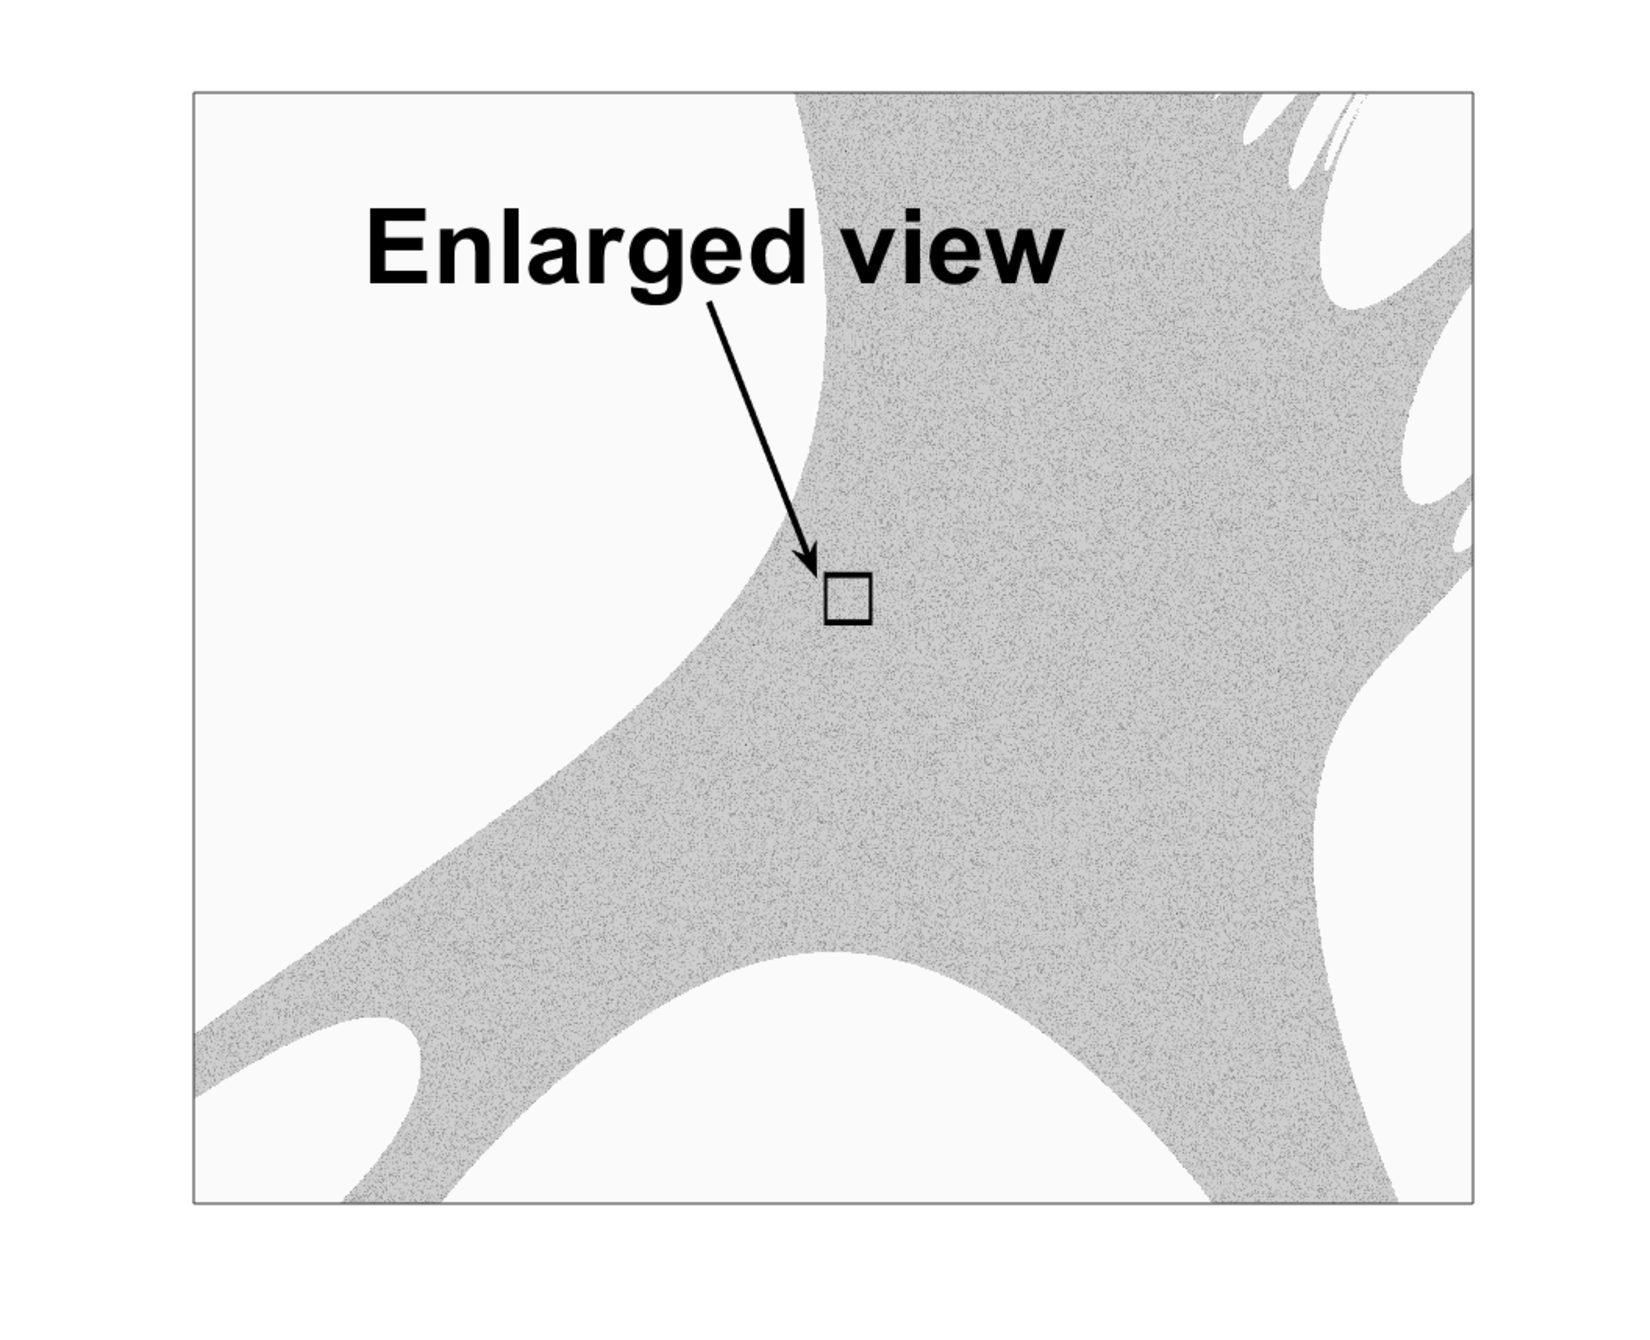
\includegraphics[width=\textwidth]{m_zoom}
        \caption{Sección rectangular del dominio de atracción, sección $[0.3\pm 0.001, -0.2\pm 0.001]$.}
        \label{fig:gull}
    \end{subfigure}
    \hfill 
    \begin{subfigure}[t]{0.49\textwidth}
        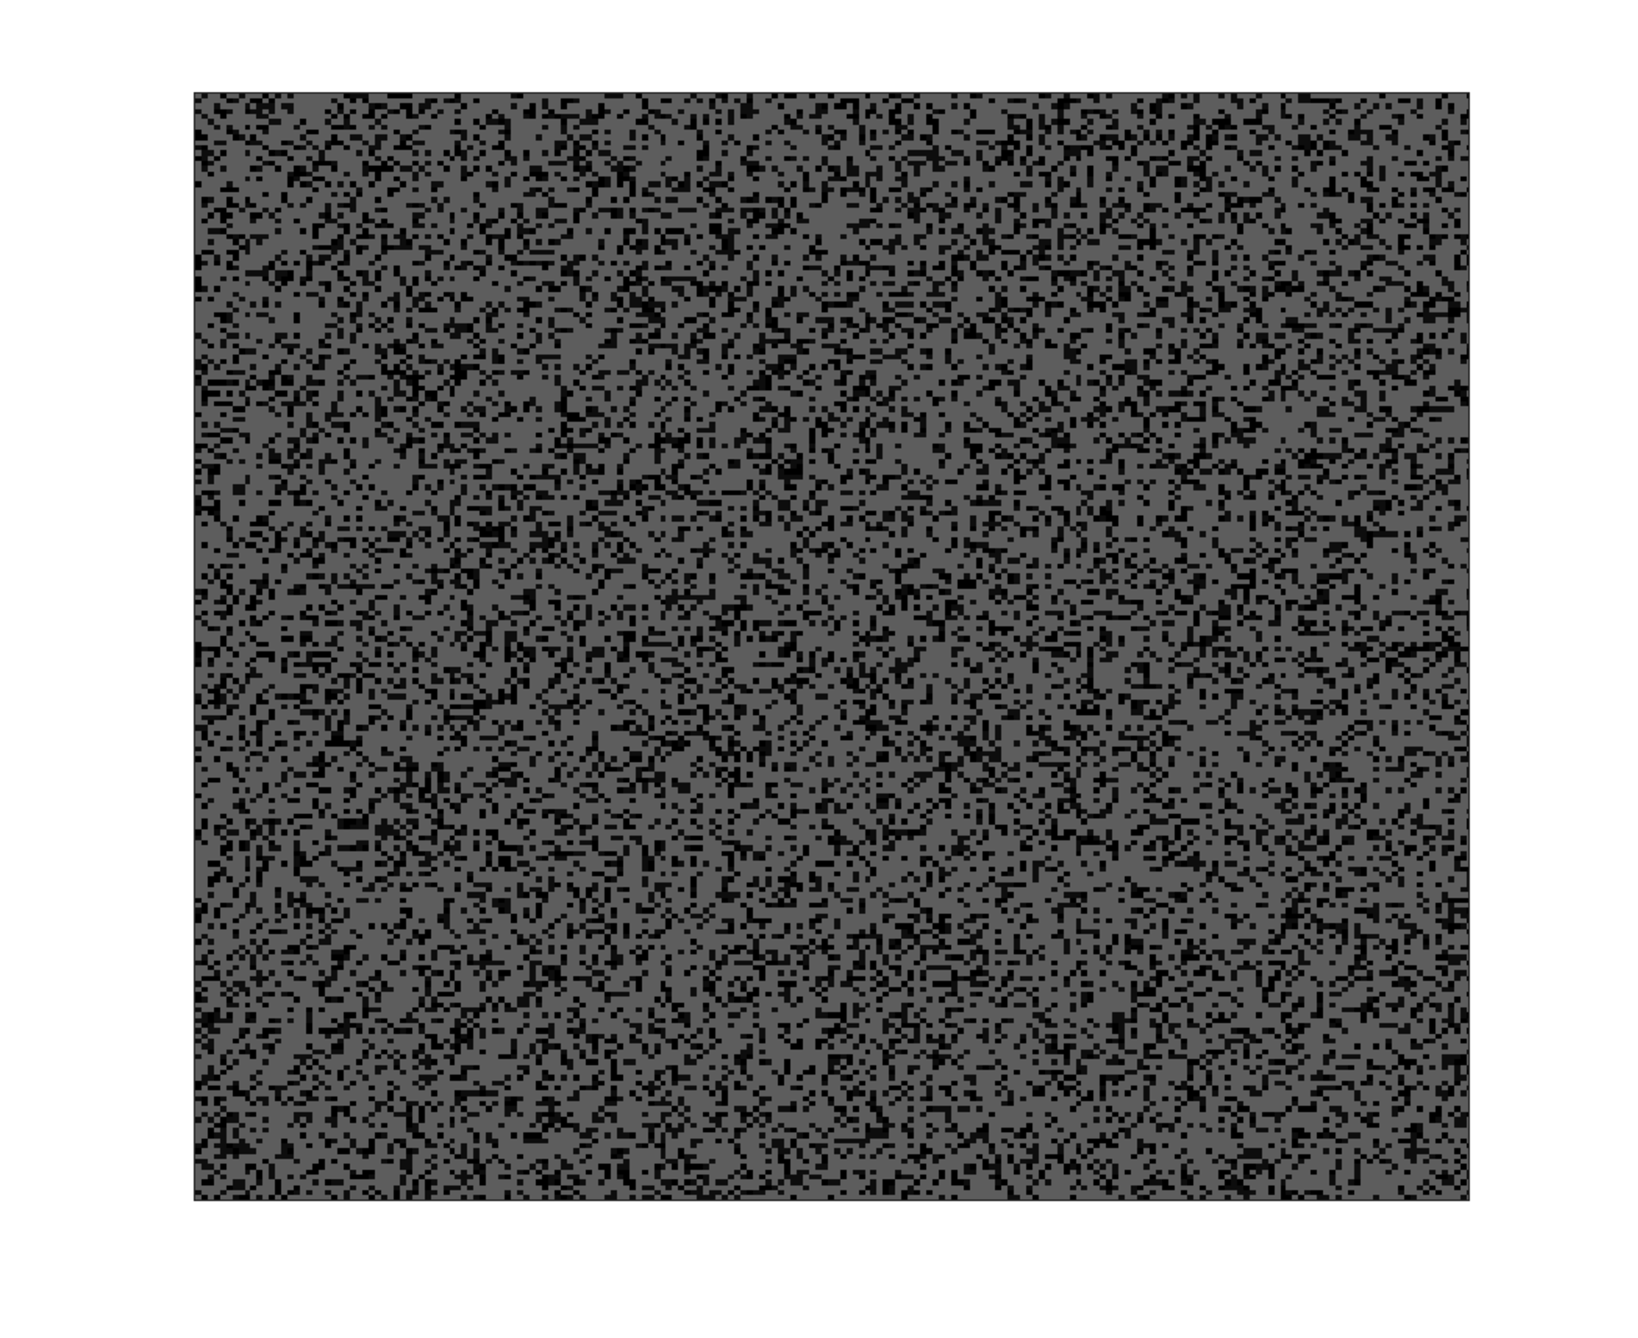
\includegraphics[width=\textwidth]{m14_lu_zoomO}
        \caption{$n_f=14$.}
        \label{fig:tiger}
    \end{subfigure}
   \hfill  
    \begin{subfigure}[t]{0.49\textwidth}
        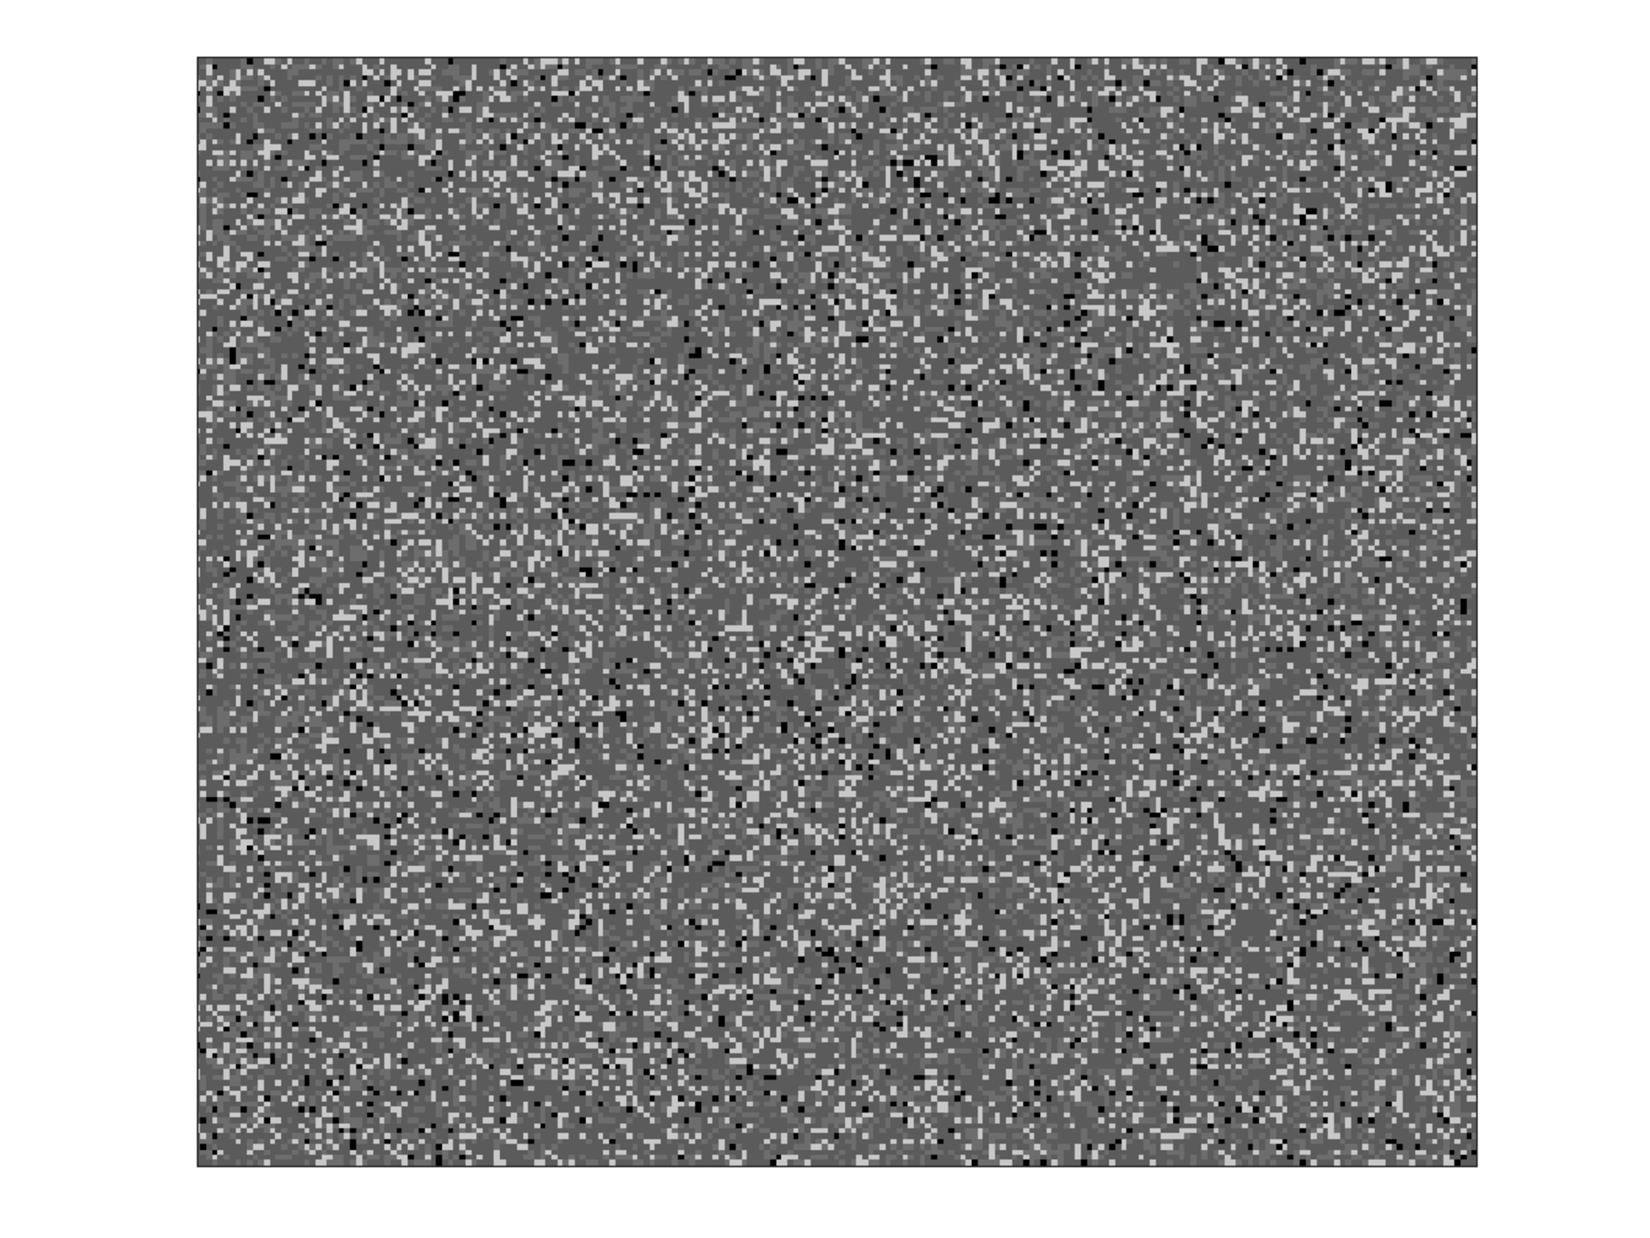
\includegraphics[width=\textwidth]{m17_lu_zoomO}
        \caption{$n_f=17$.}
        \label{fig:mouse}
    \end{subfigure}
  \hfill   
    \begin{subfigure}[t]{0.49\textwidth}
        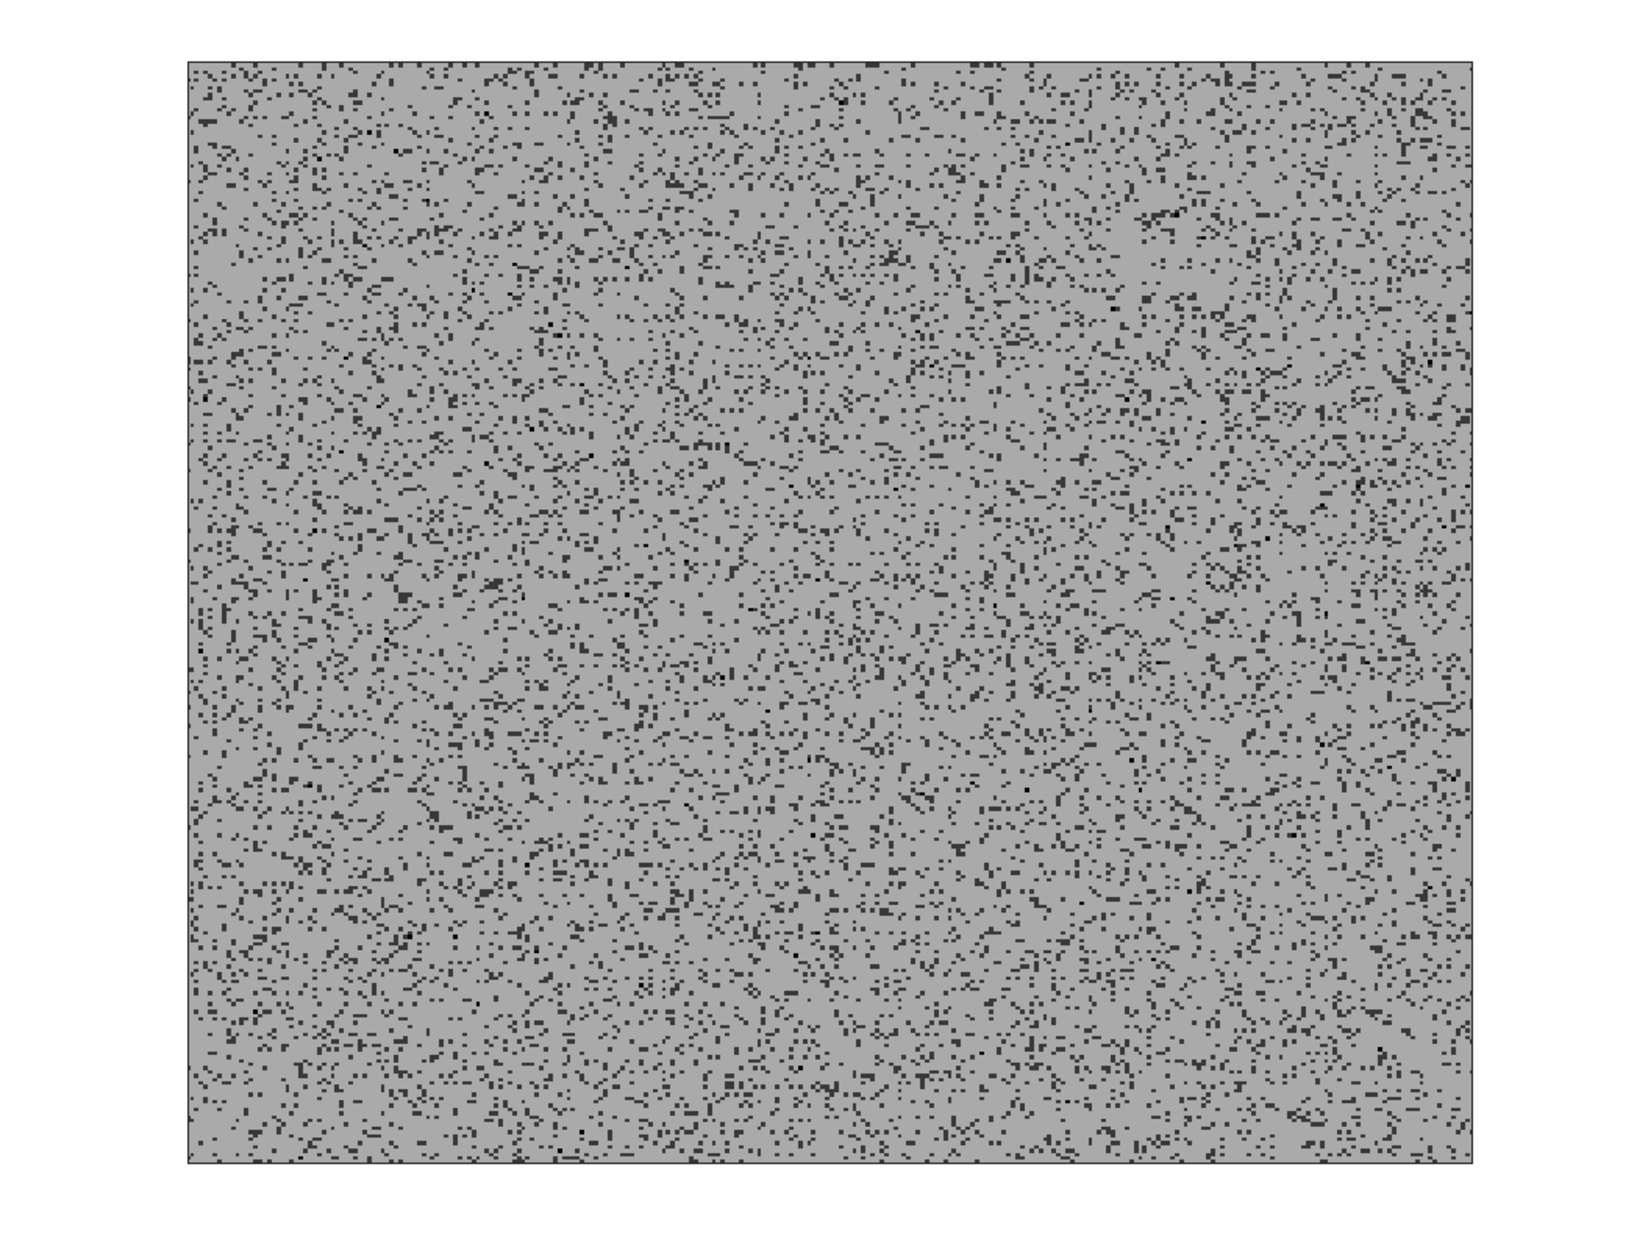
\includegraphics[width=\textwidth]{m18_lu_zoomO}
        \caption{$n_f=18$.}
        \label{fig:mouse}
    \end{subfigure}
    \caption{Vistas ampliadas del dominio de atracción para distintos valores de $n_f$.}\label{fig:m_zoom}
\end{figure}

Sin embargo, cuando queremos hacer una comparación general de lo que ocurre con los períodos en los que las precisiones son variadas, se requiere una escala de colores, ver Fig.\ref{fig:m}.
%
\begin{figure*}
\centering
\begin{tabular}{cc}
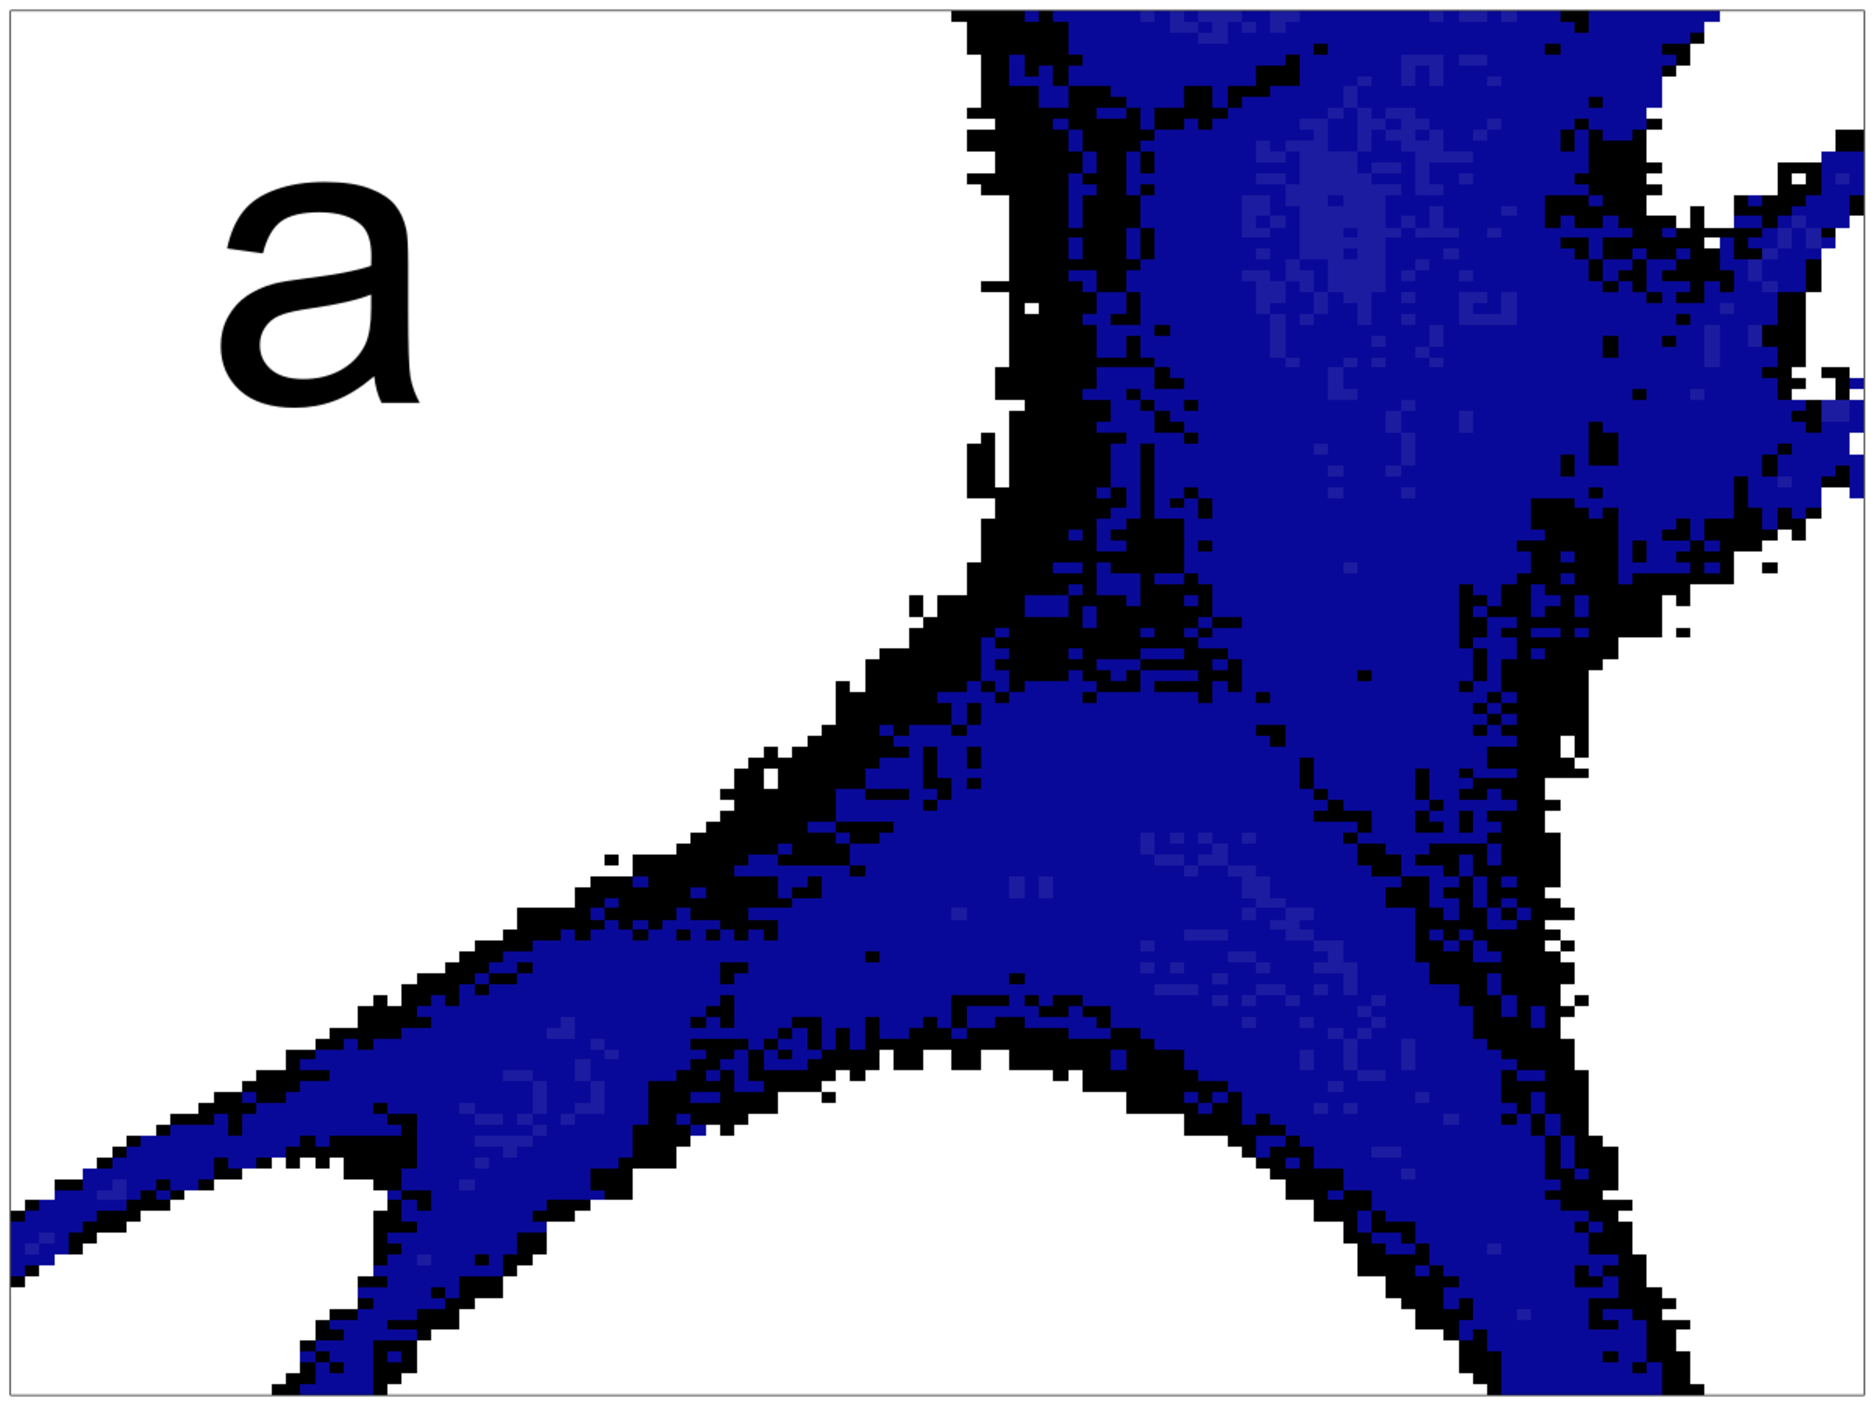
\includegraphics[width=0.35\textwidth]{m5}
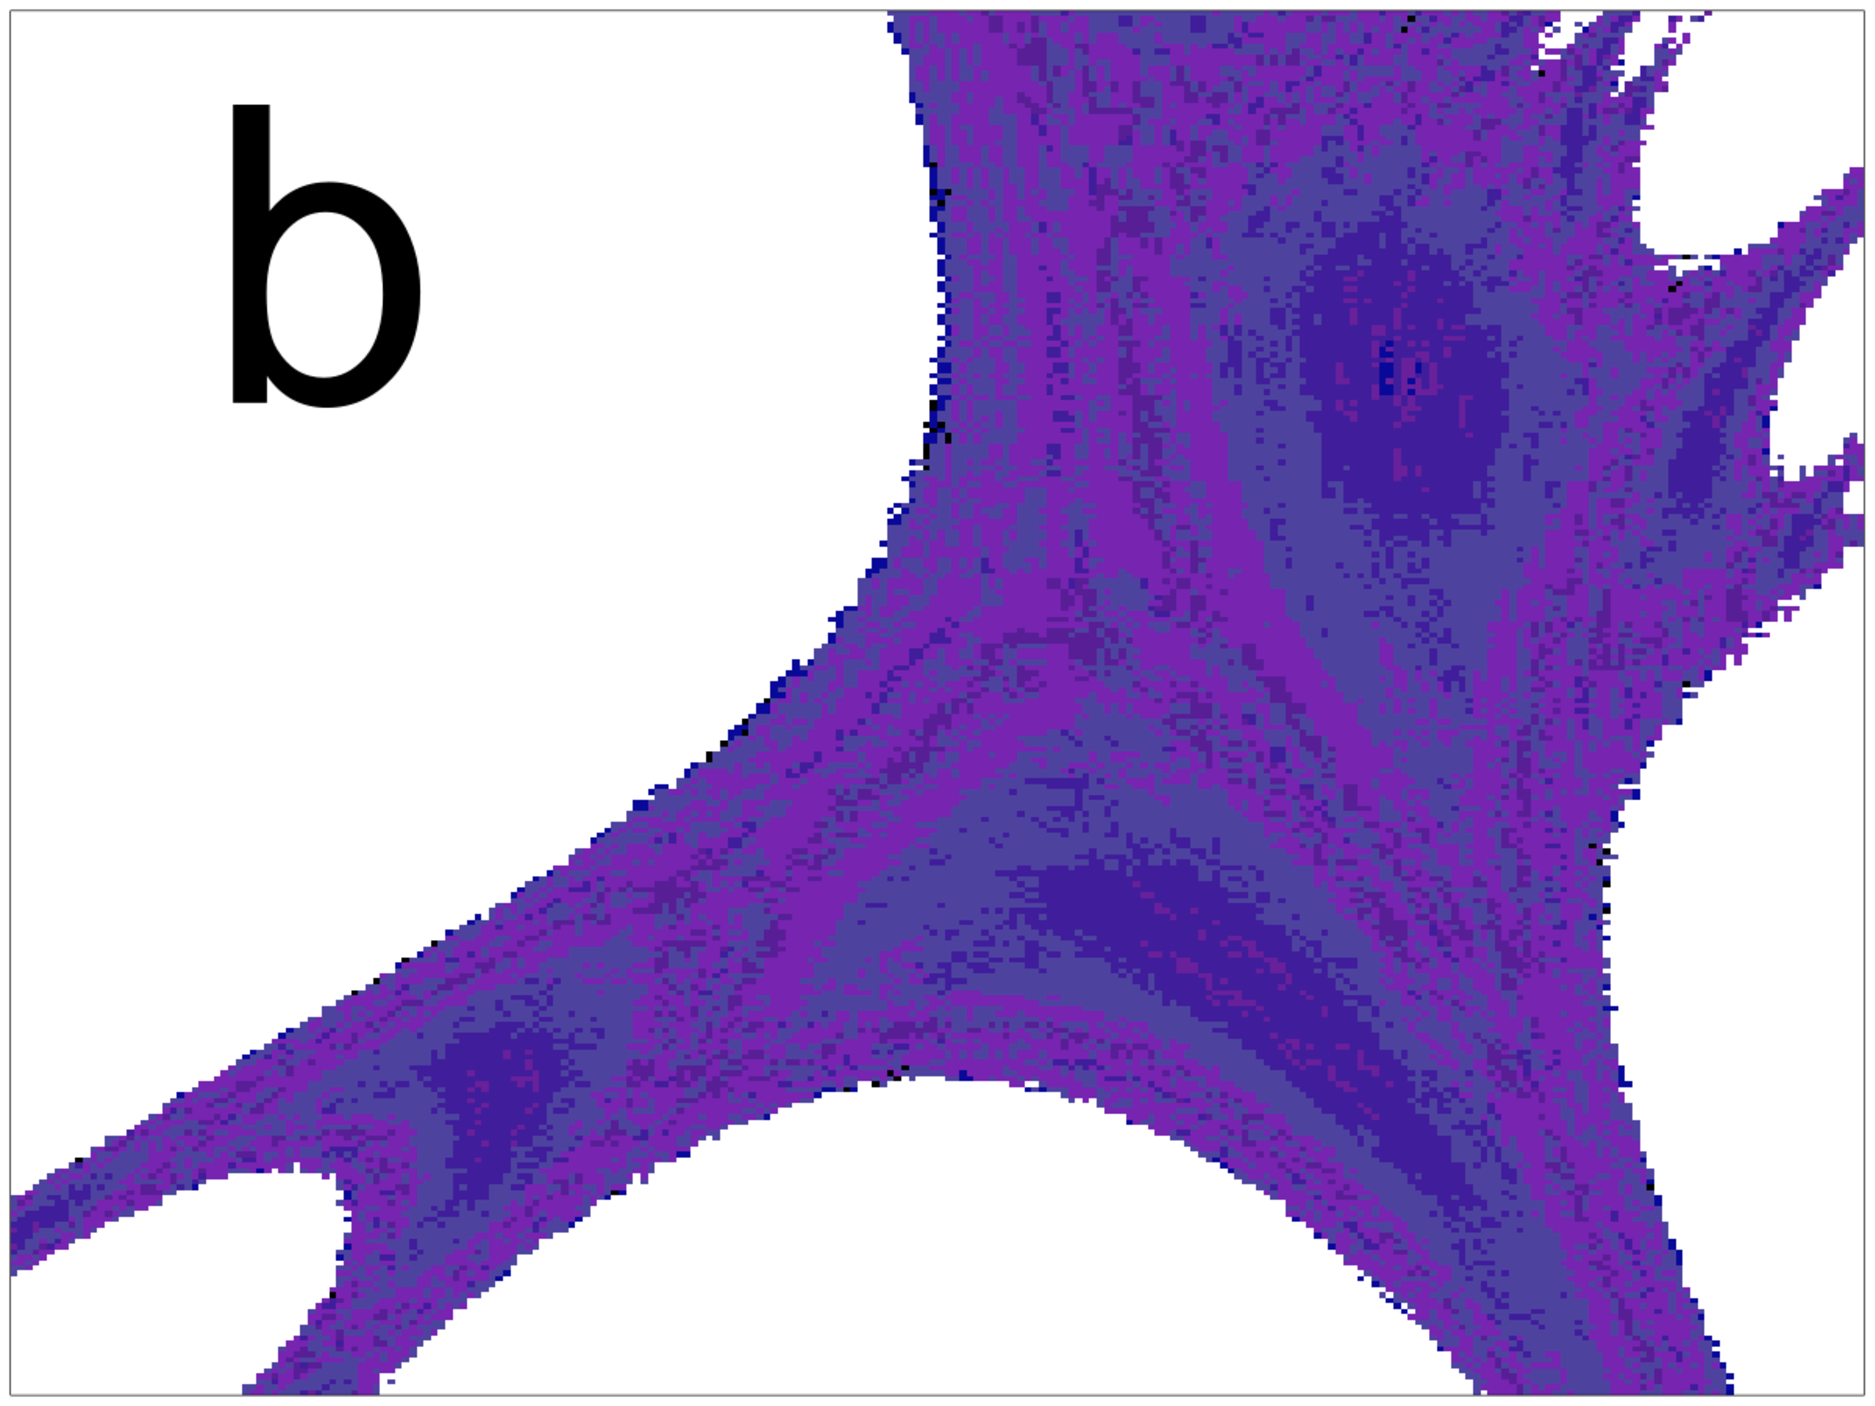
\includegraphics[width=0.35\textwidth]{m6}
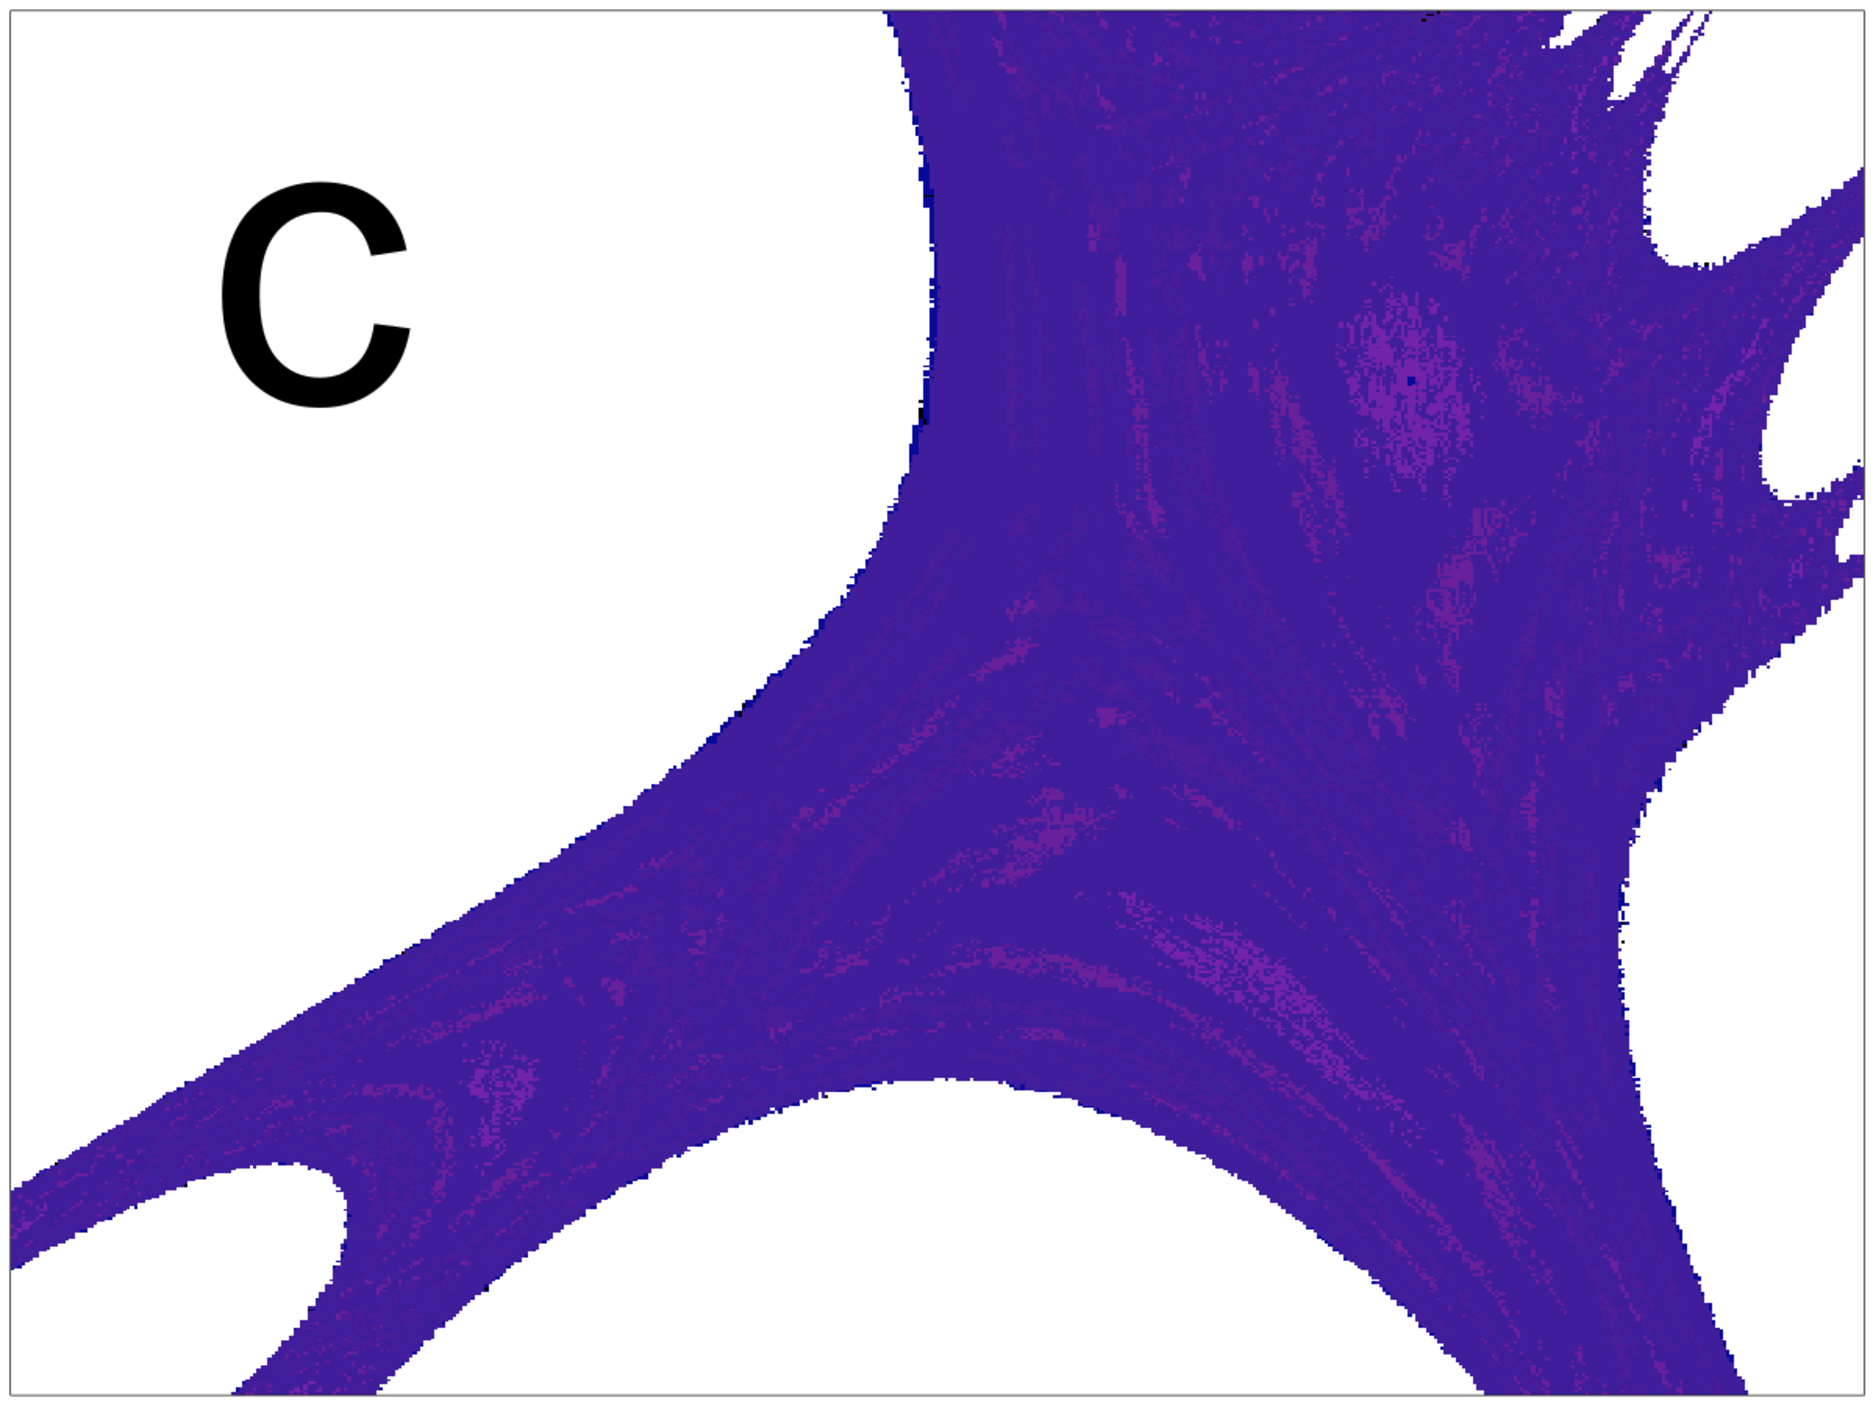
\includegraphics[width=0.35\textwidth]{m7}\\
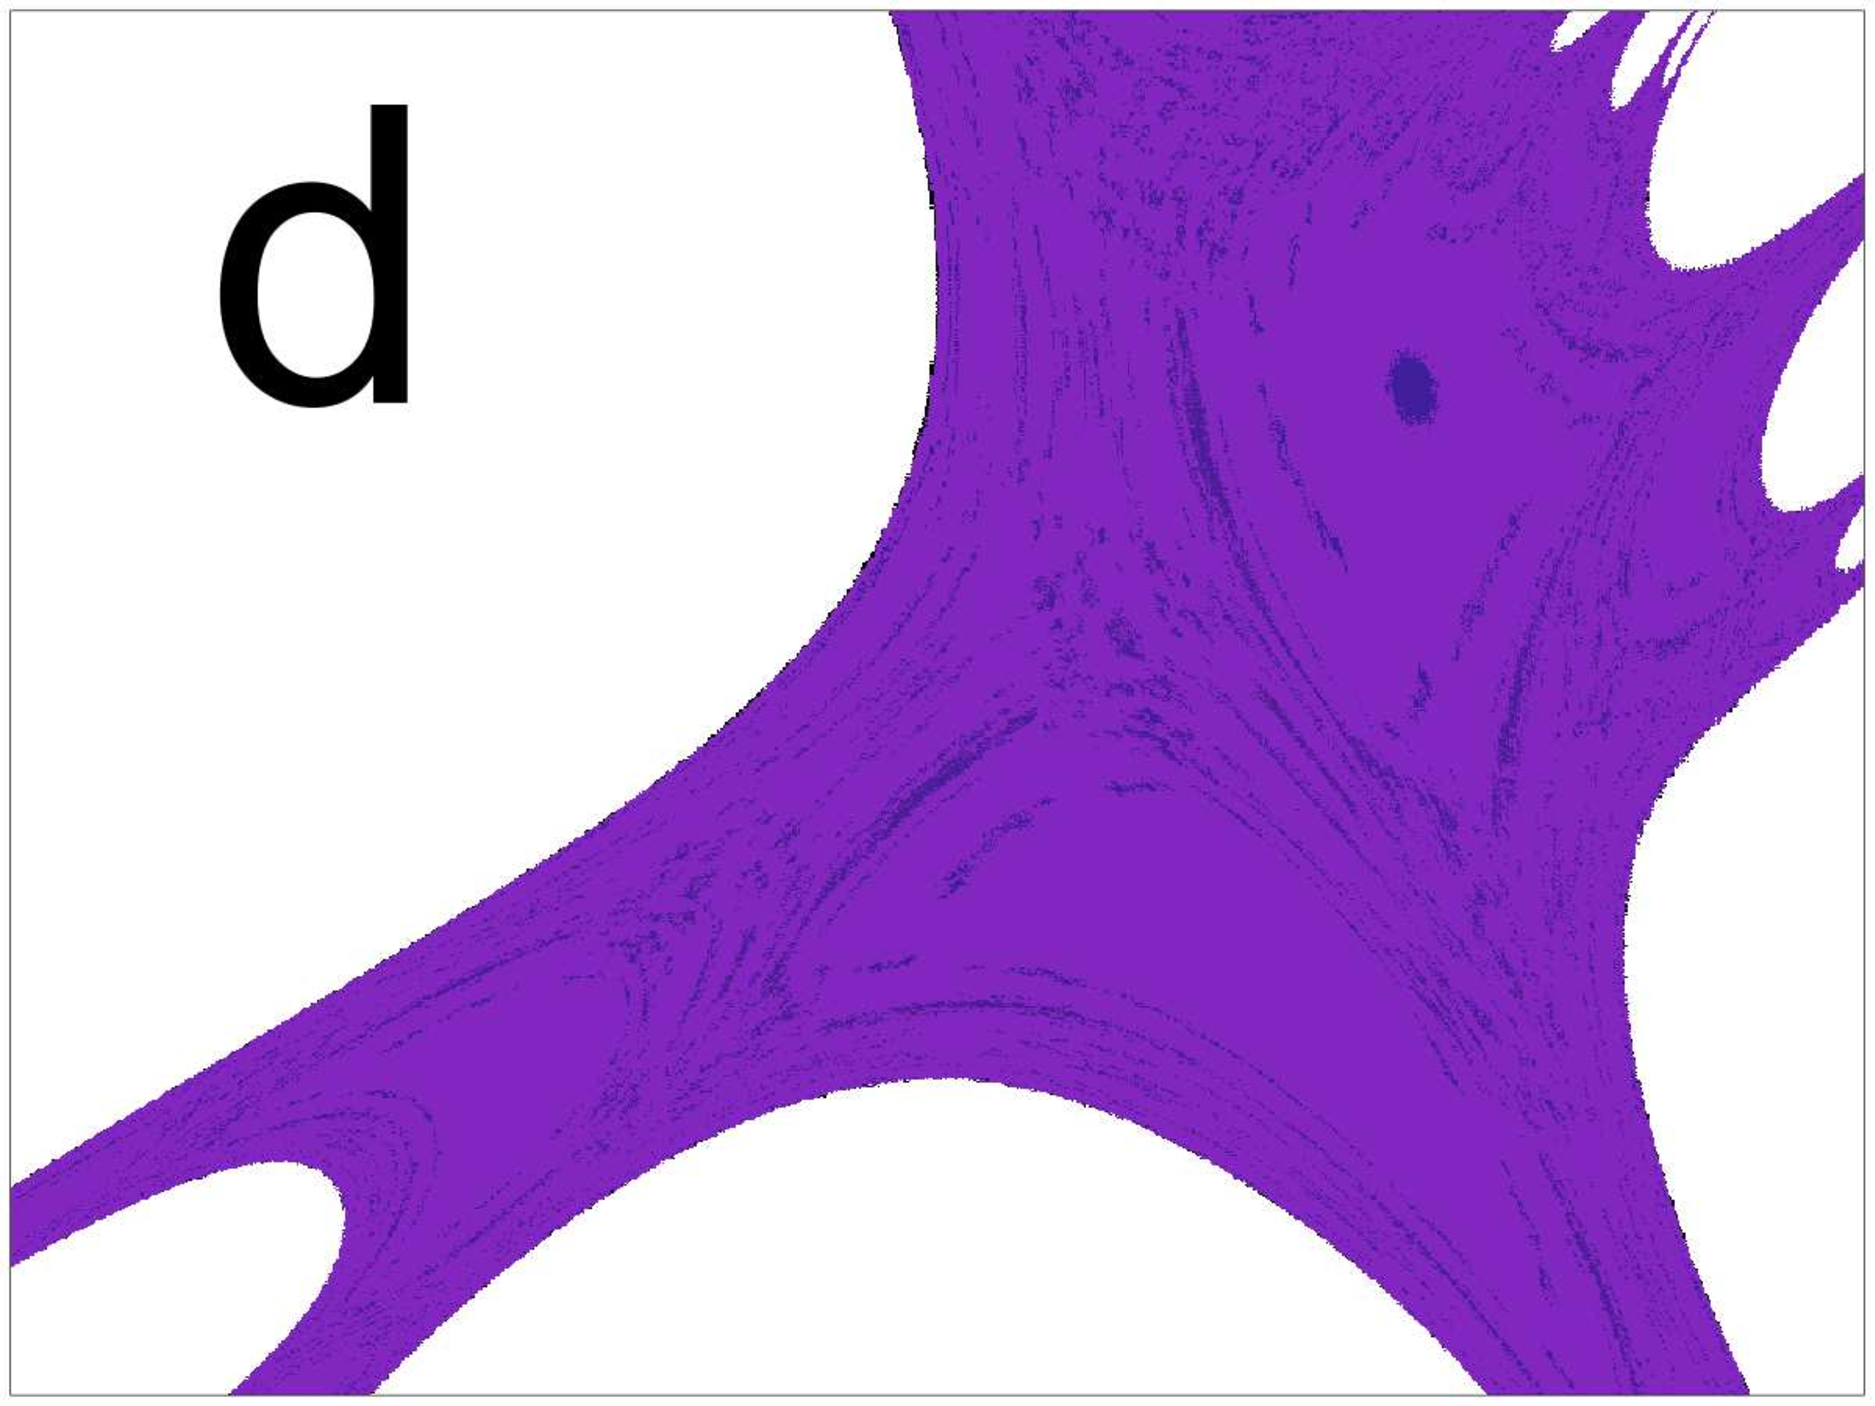
\includegraphics[width=0.35\textwidth]{m8}
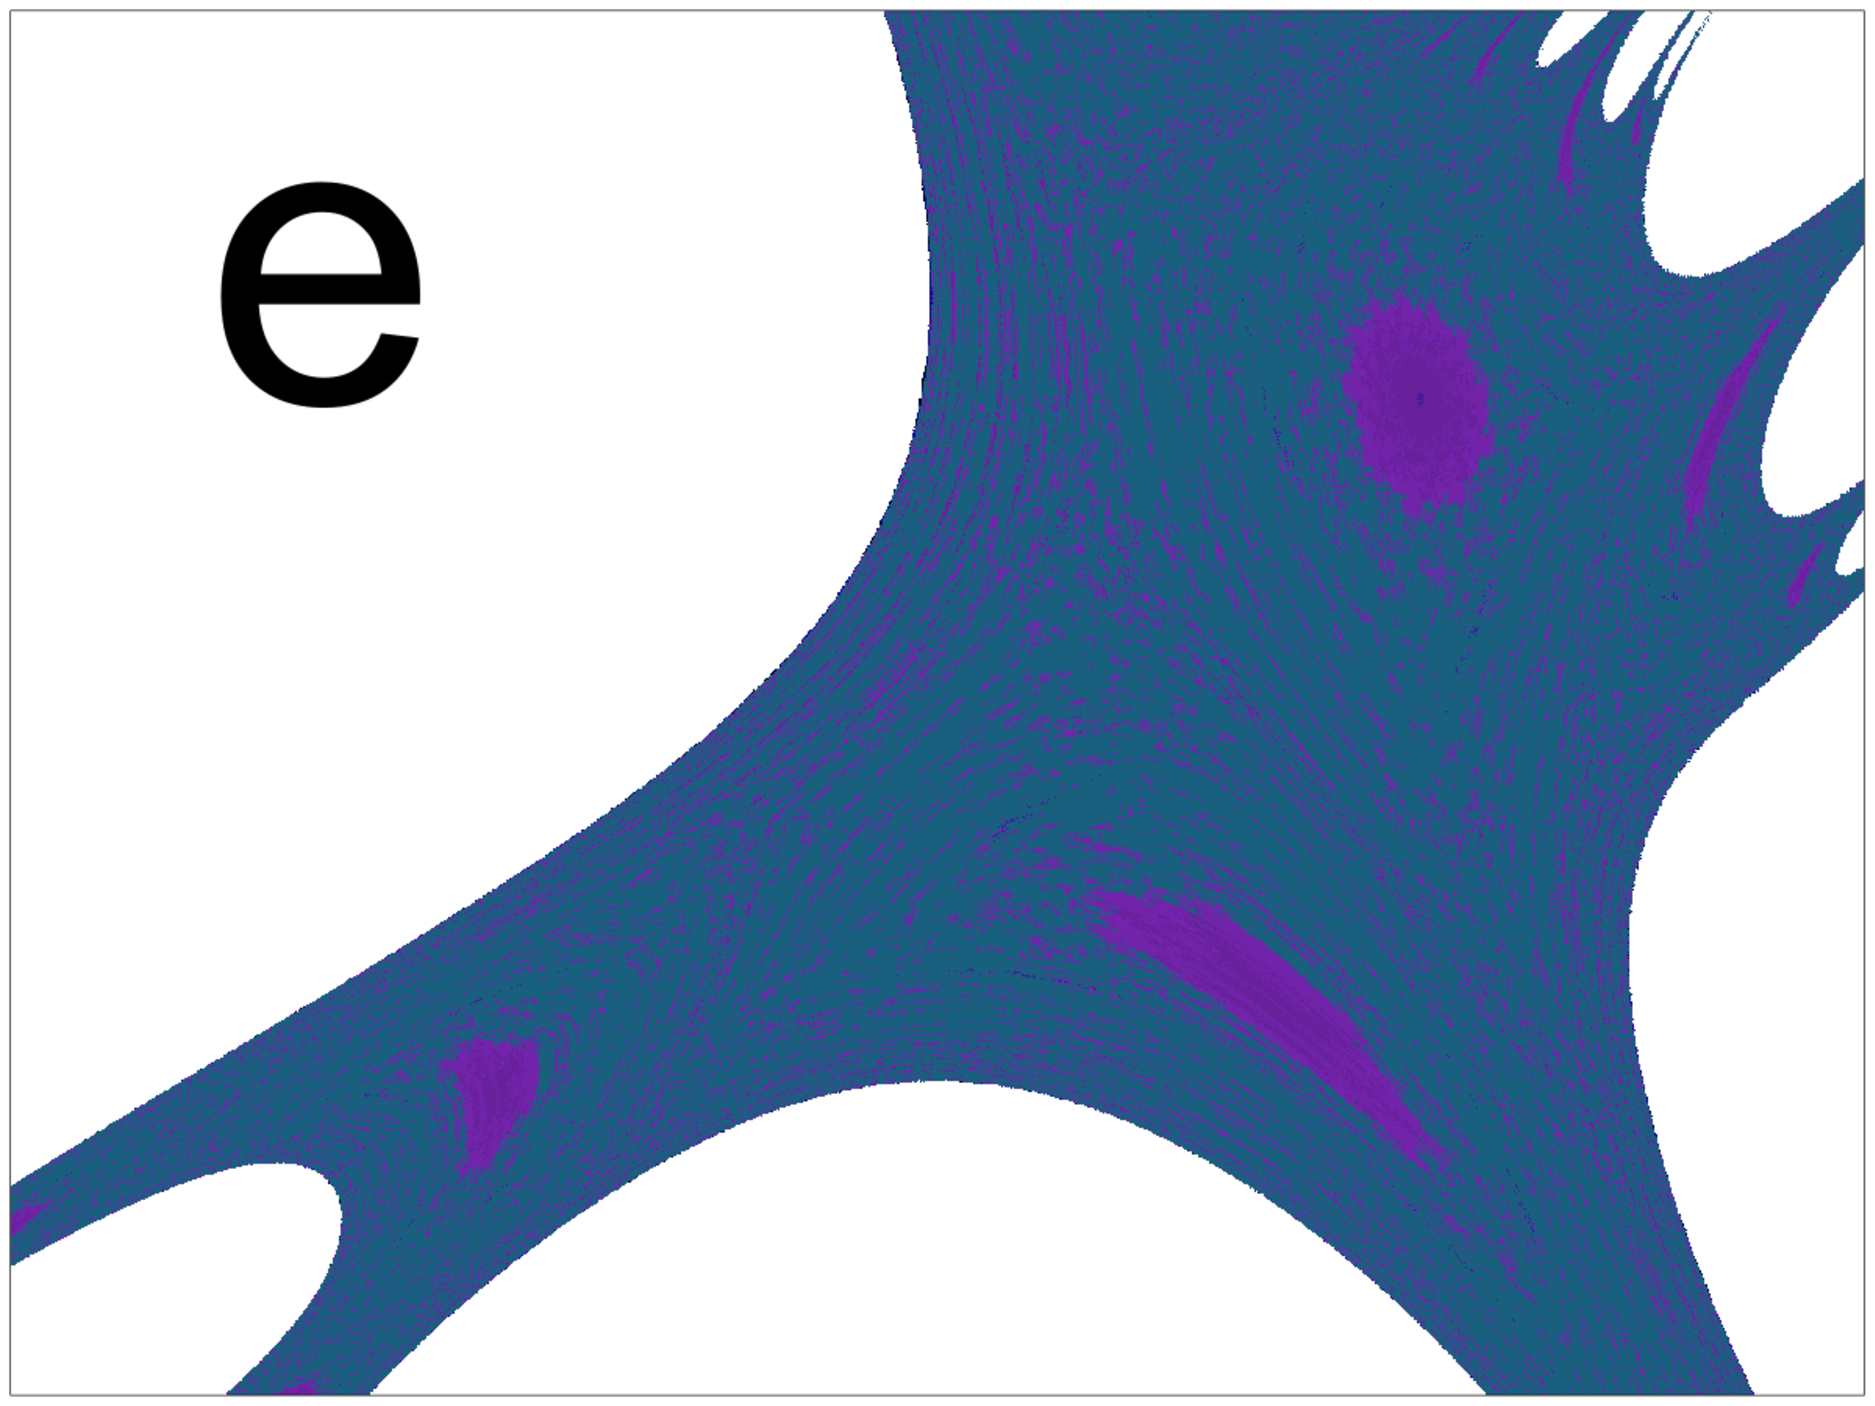
\includegraphics[width=0.35\textwidth]{m9}
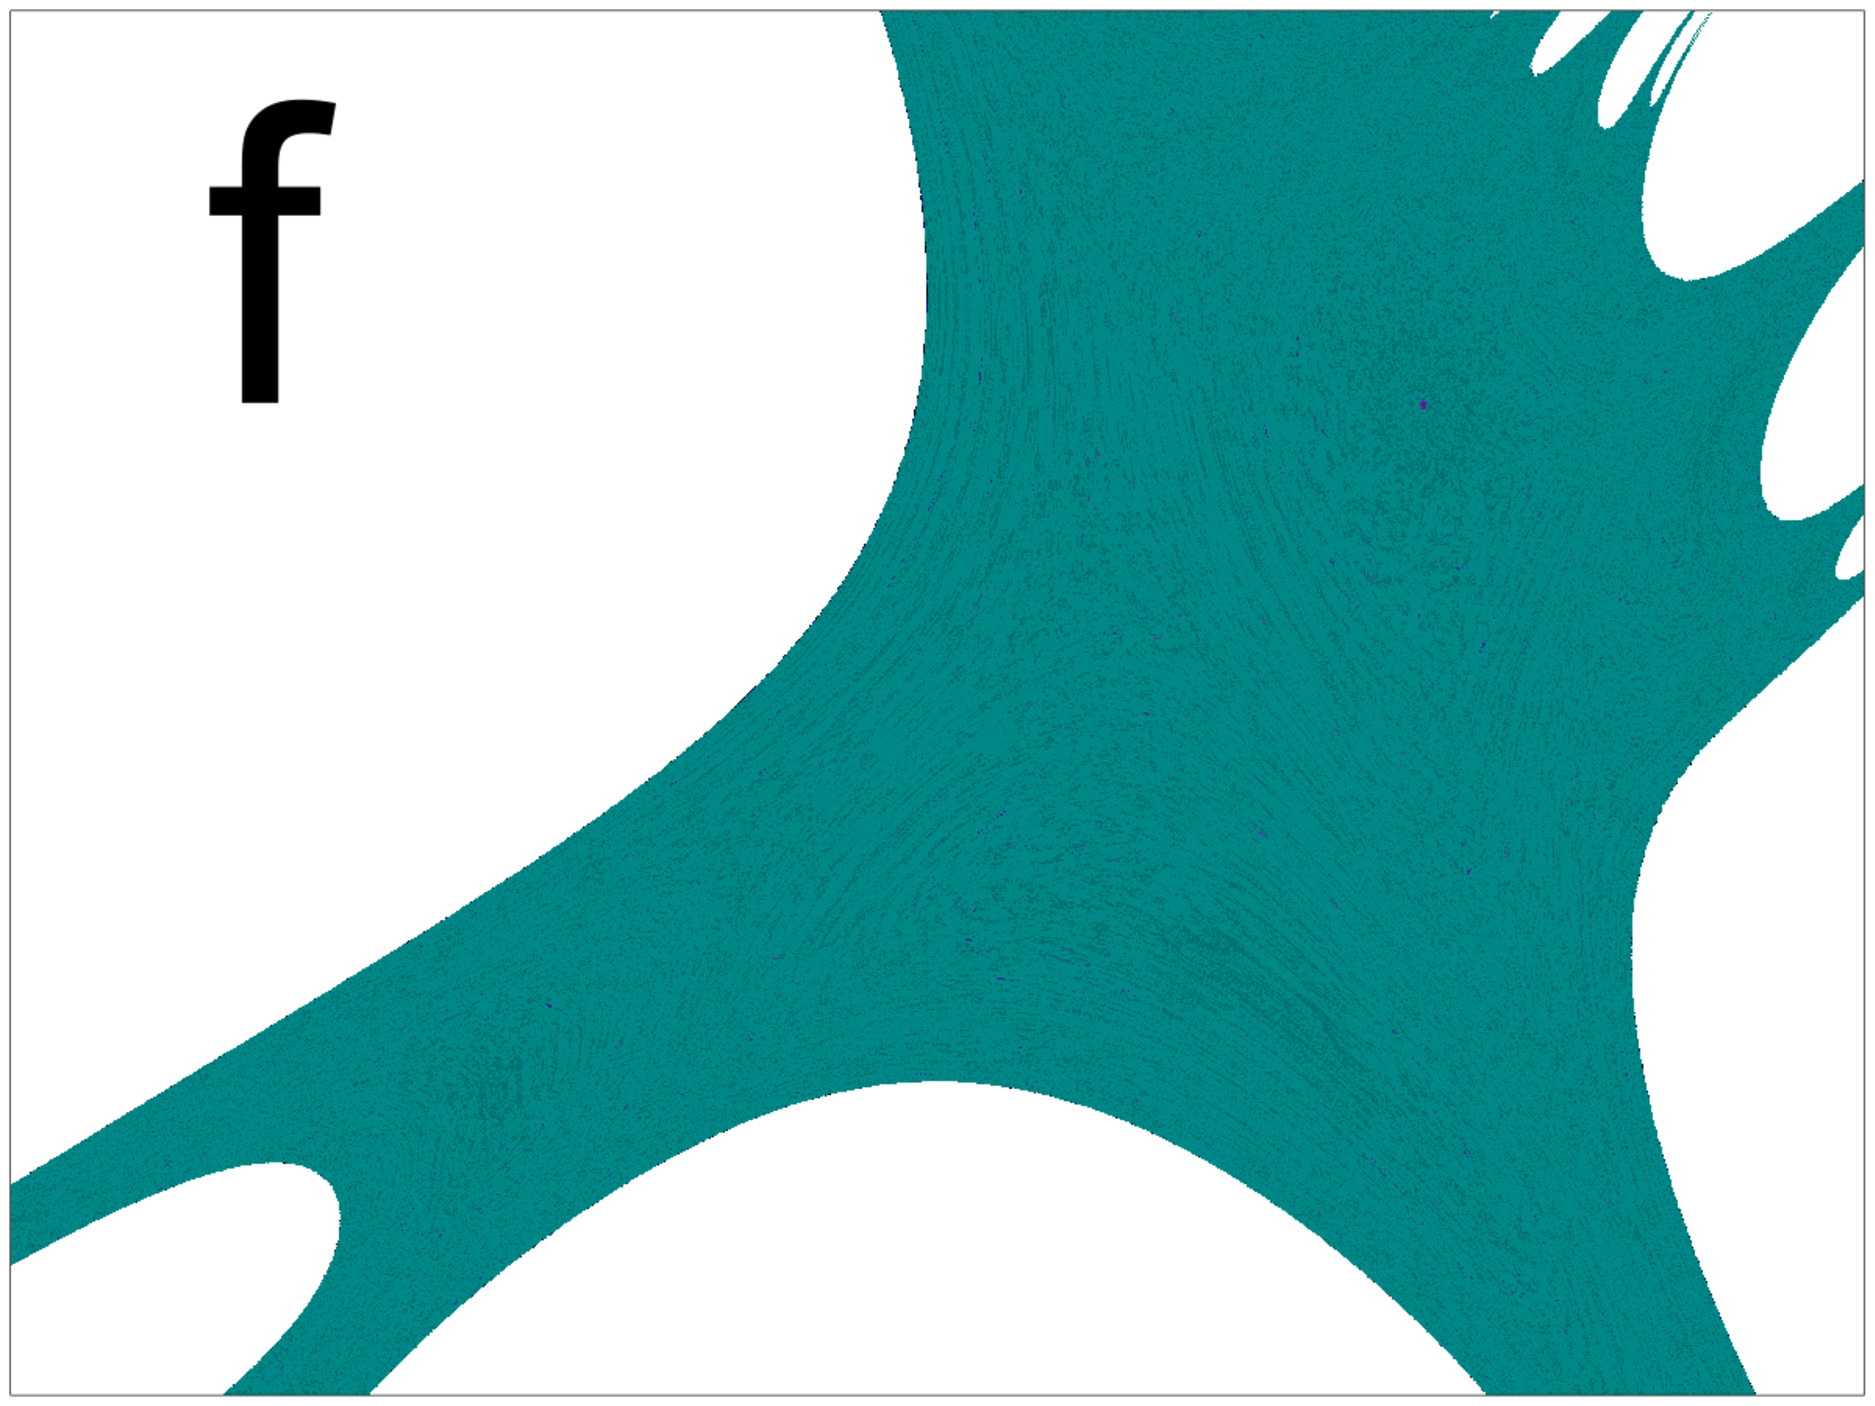
\includegraphics[width=0.35\textwidth]{m10}\\
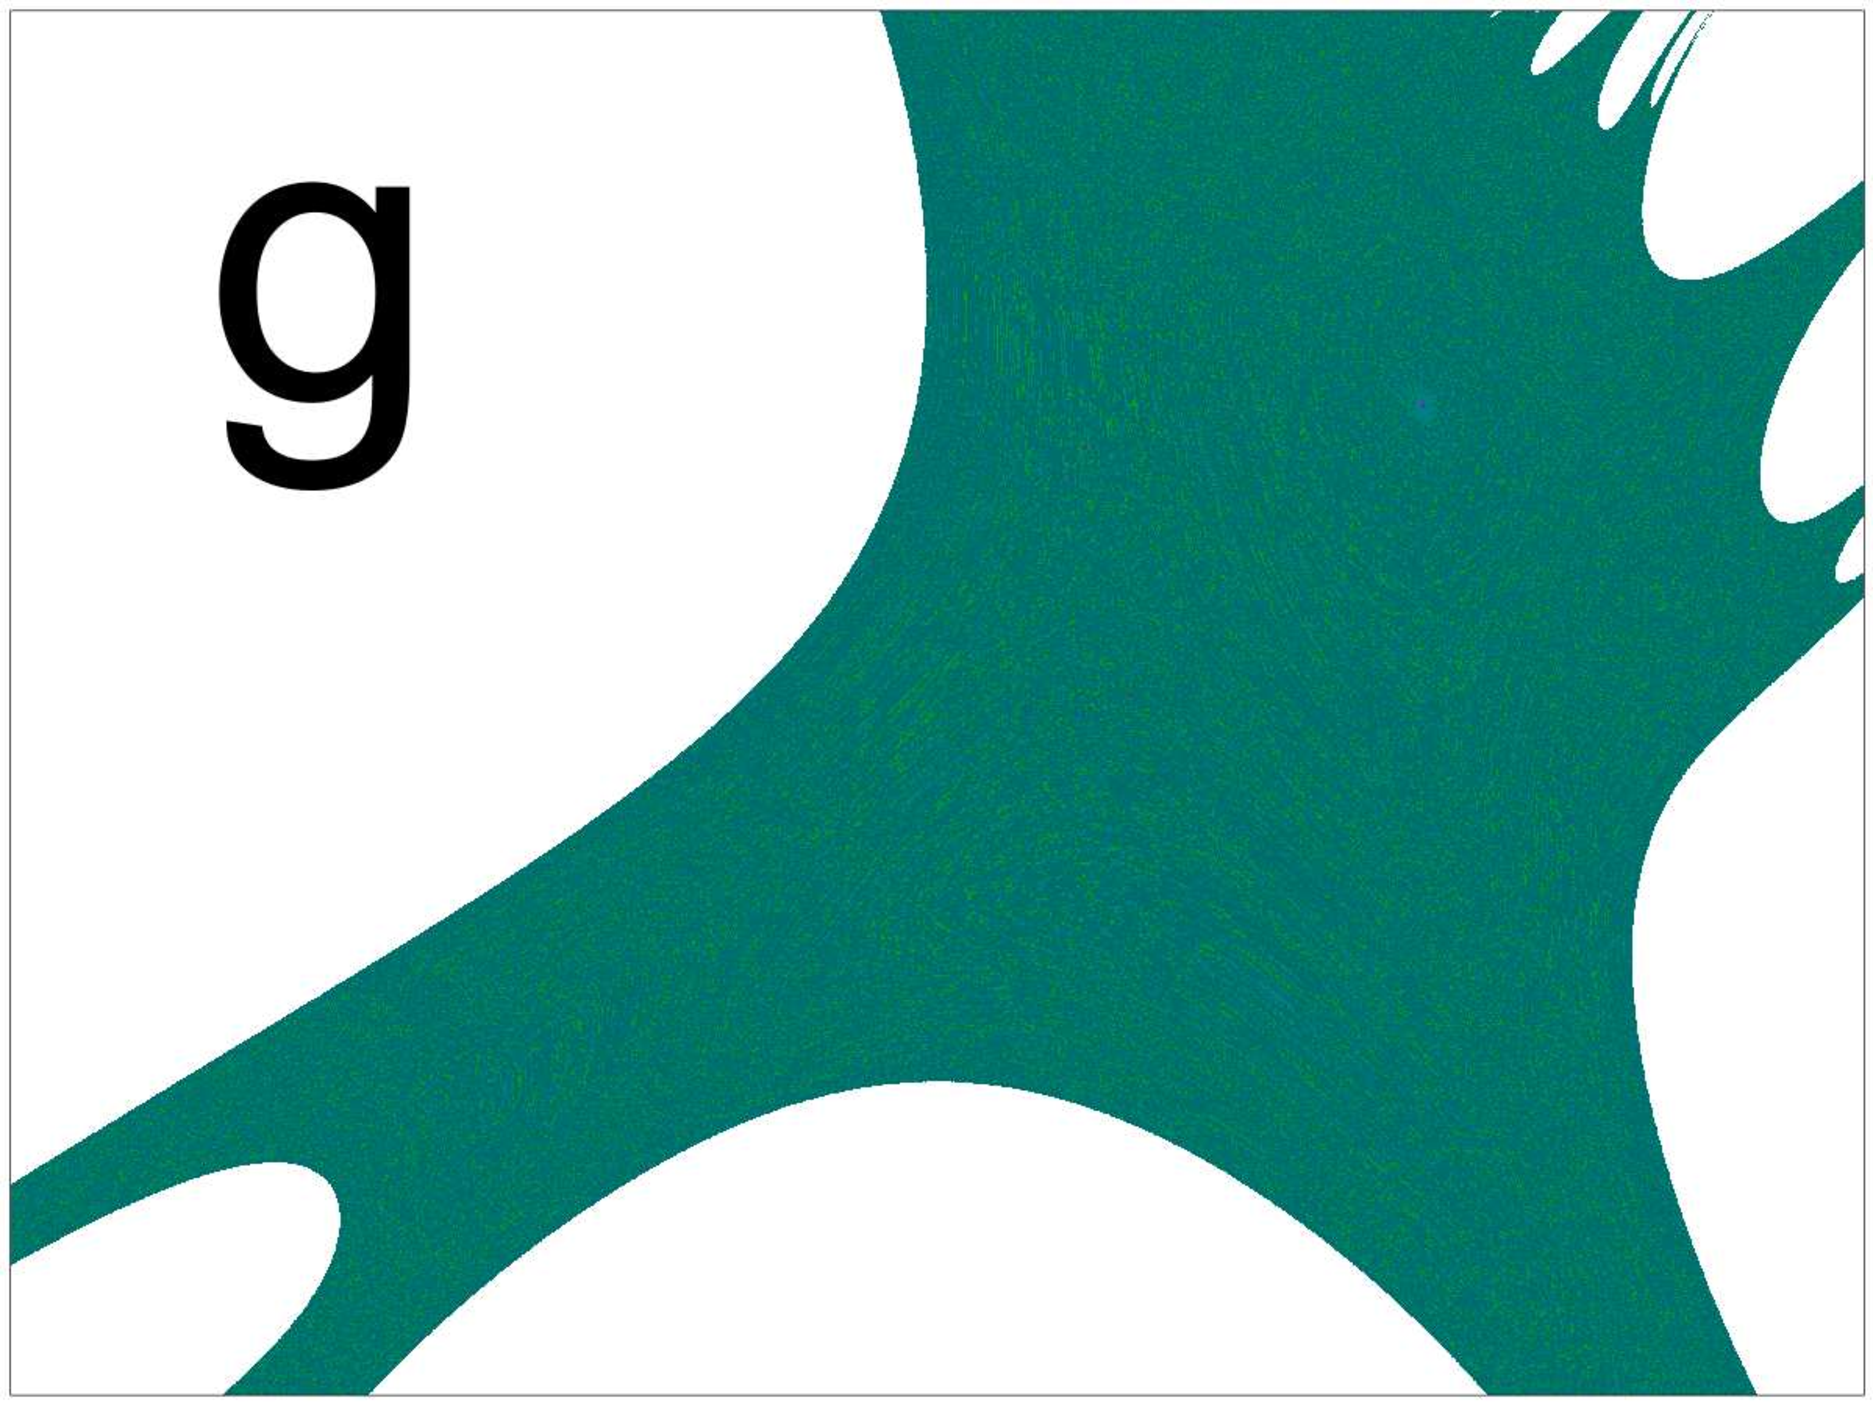
\includegraphics[width=0.35\textwidth]{m11}
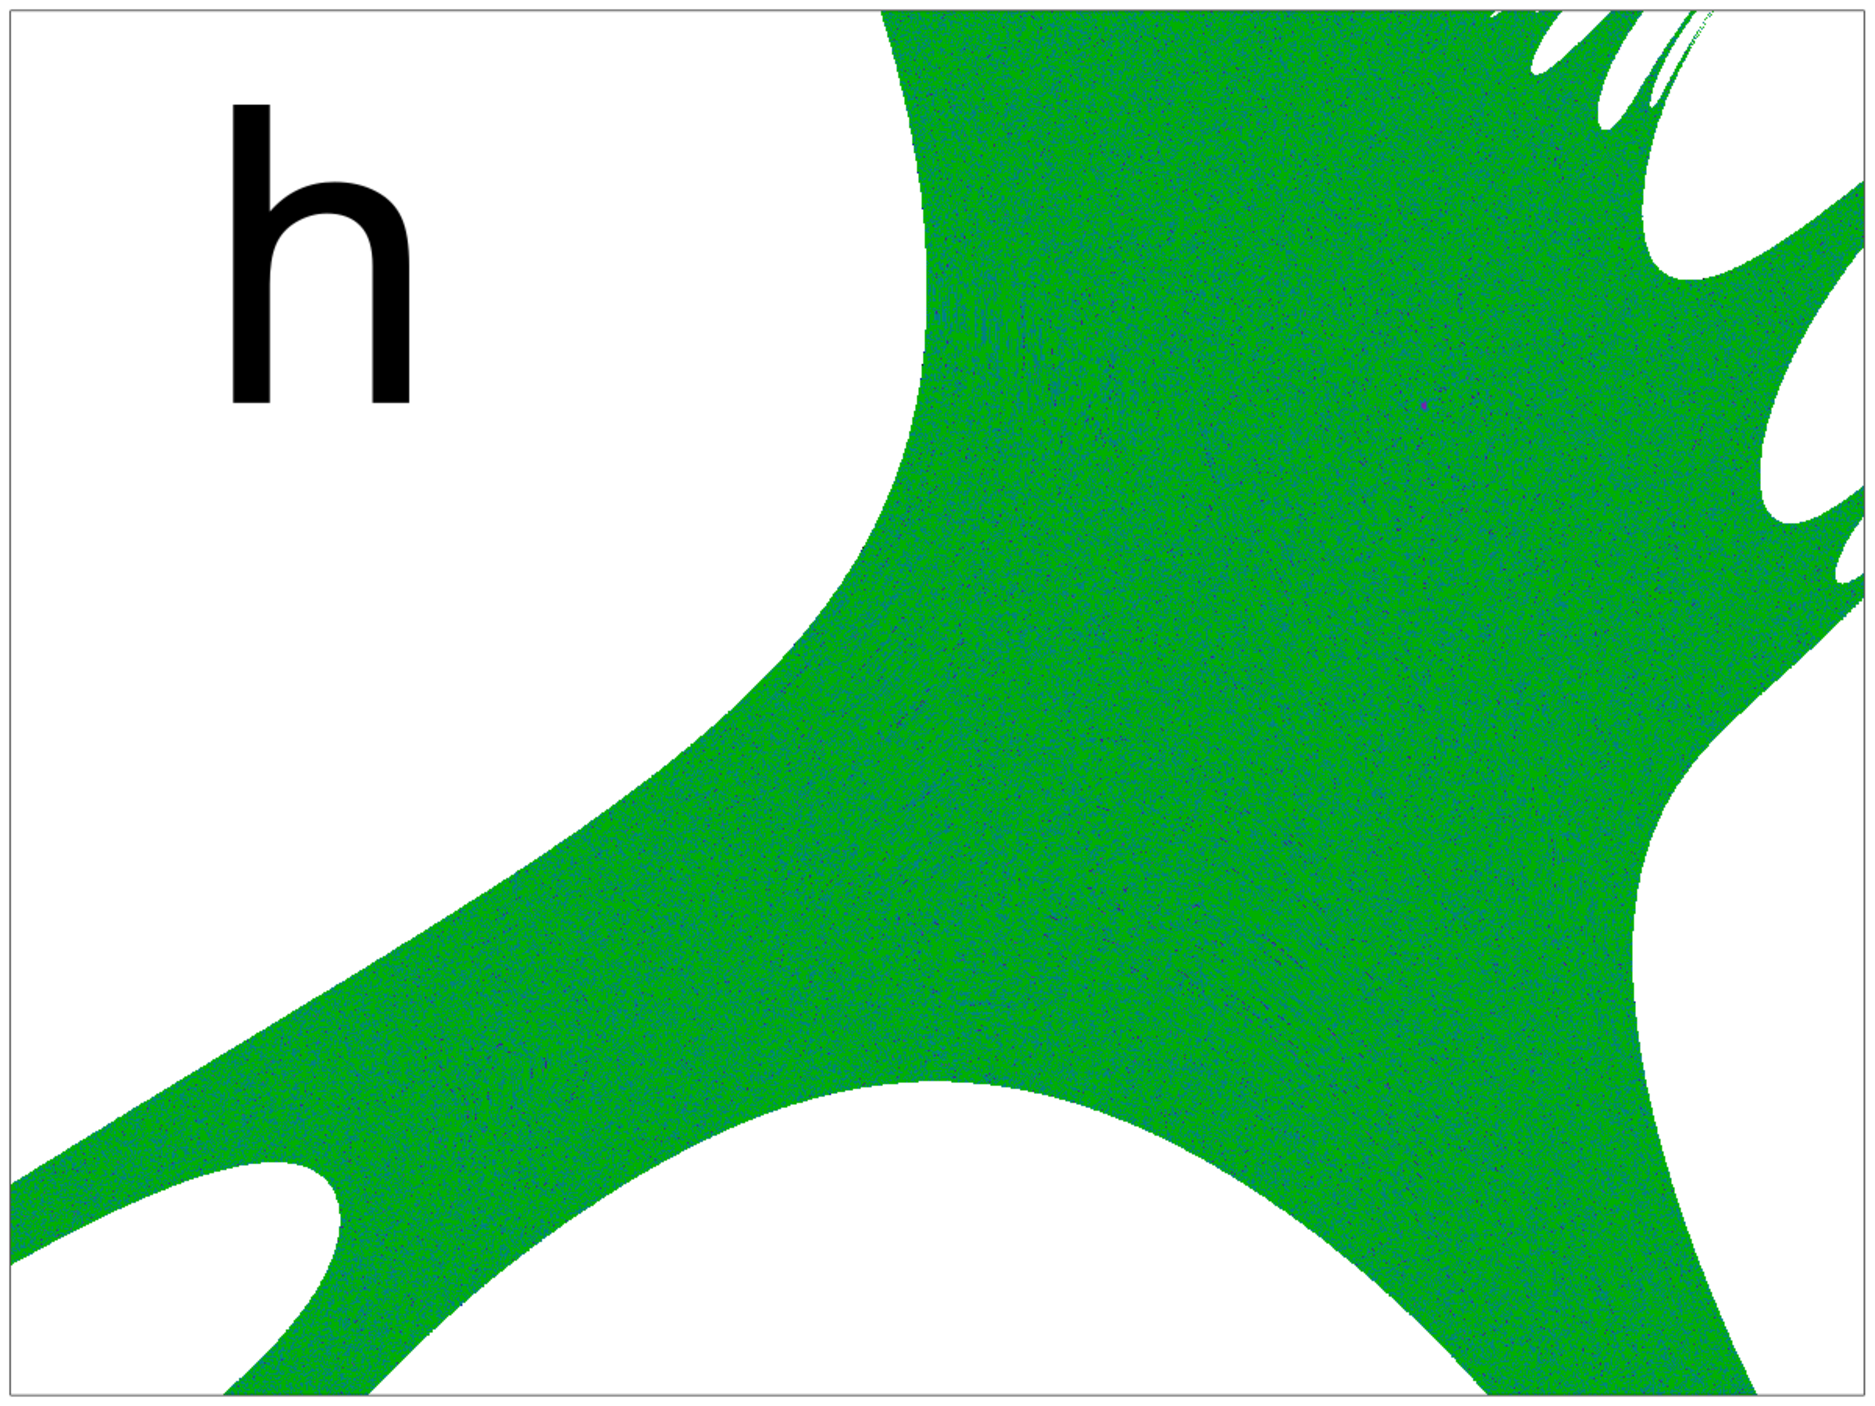
\includegraphics[width=0.35\textwidth]{m12}

\includegraphics[width=0.35\textwidth]{m13}\\
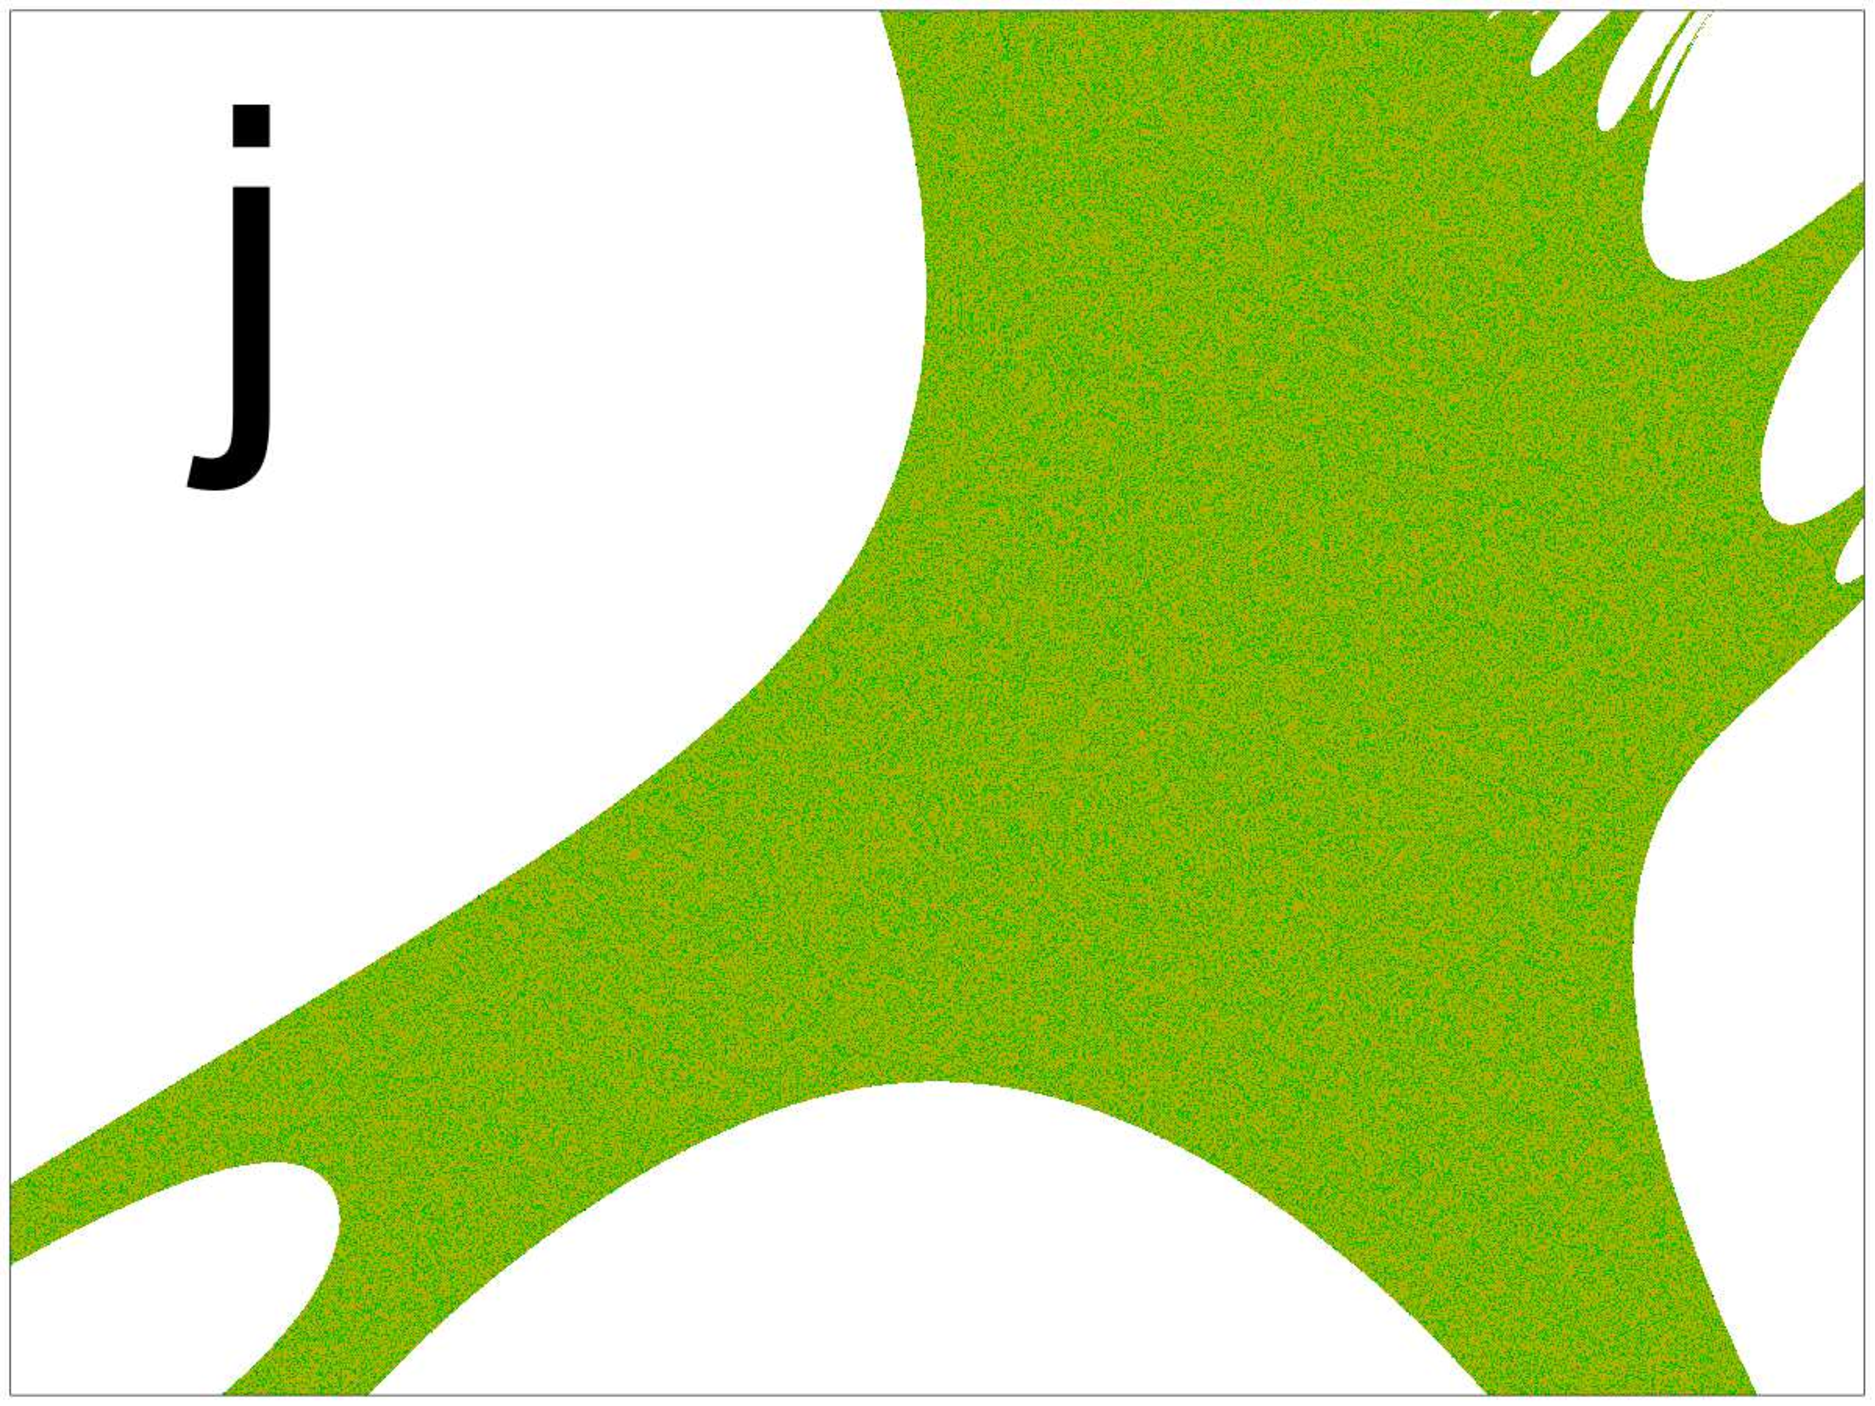
\includegraphics[width=0.35\textwidth]{m14}
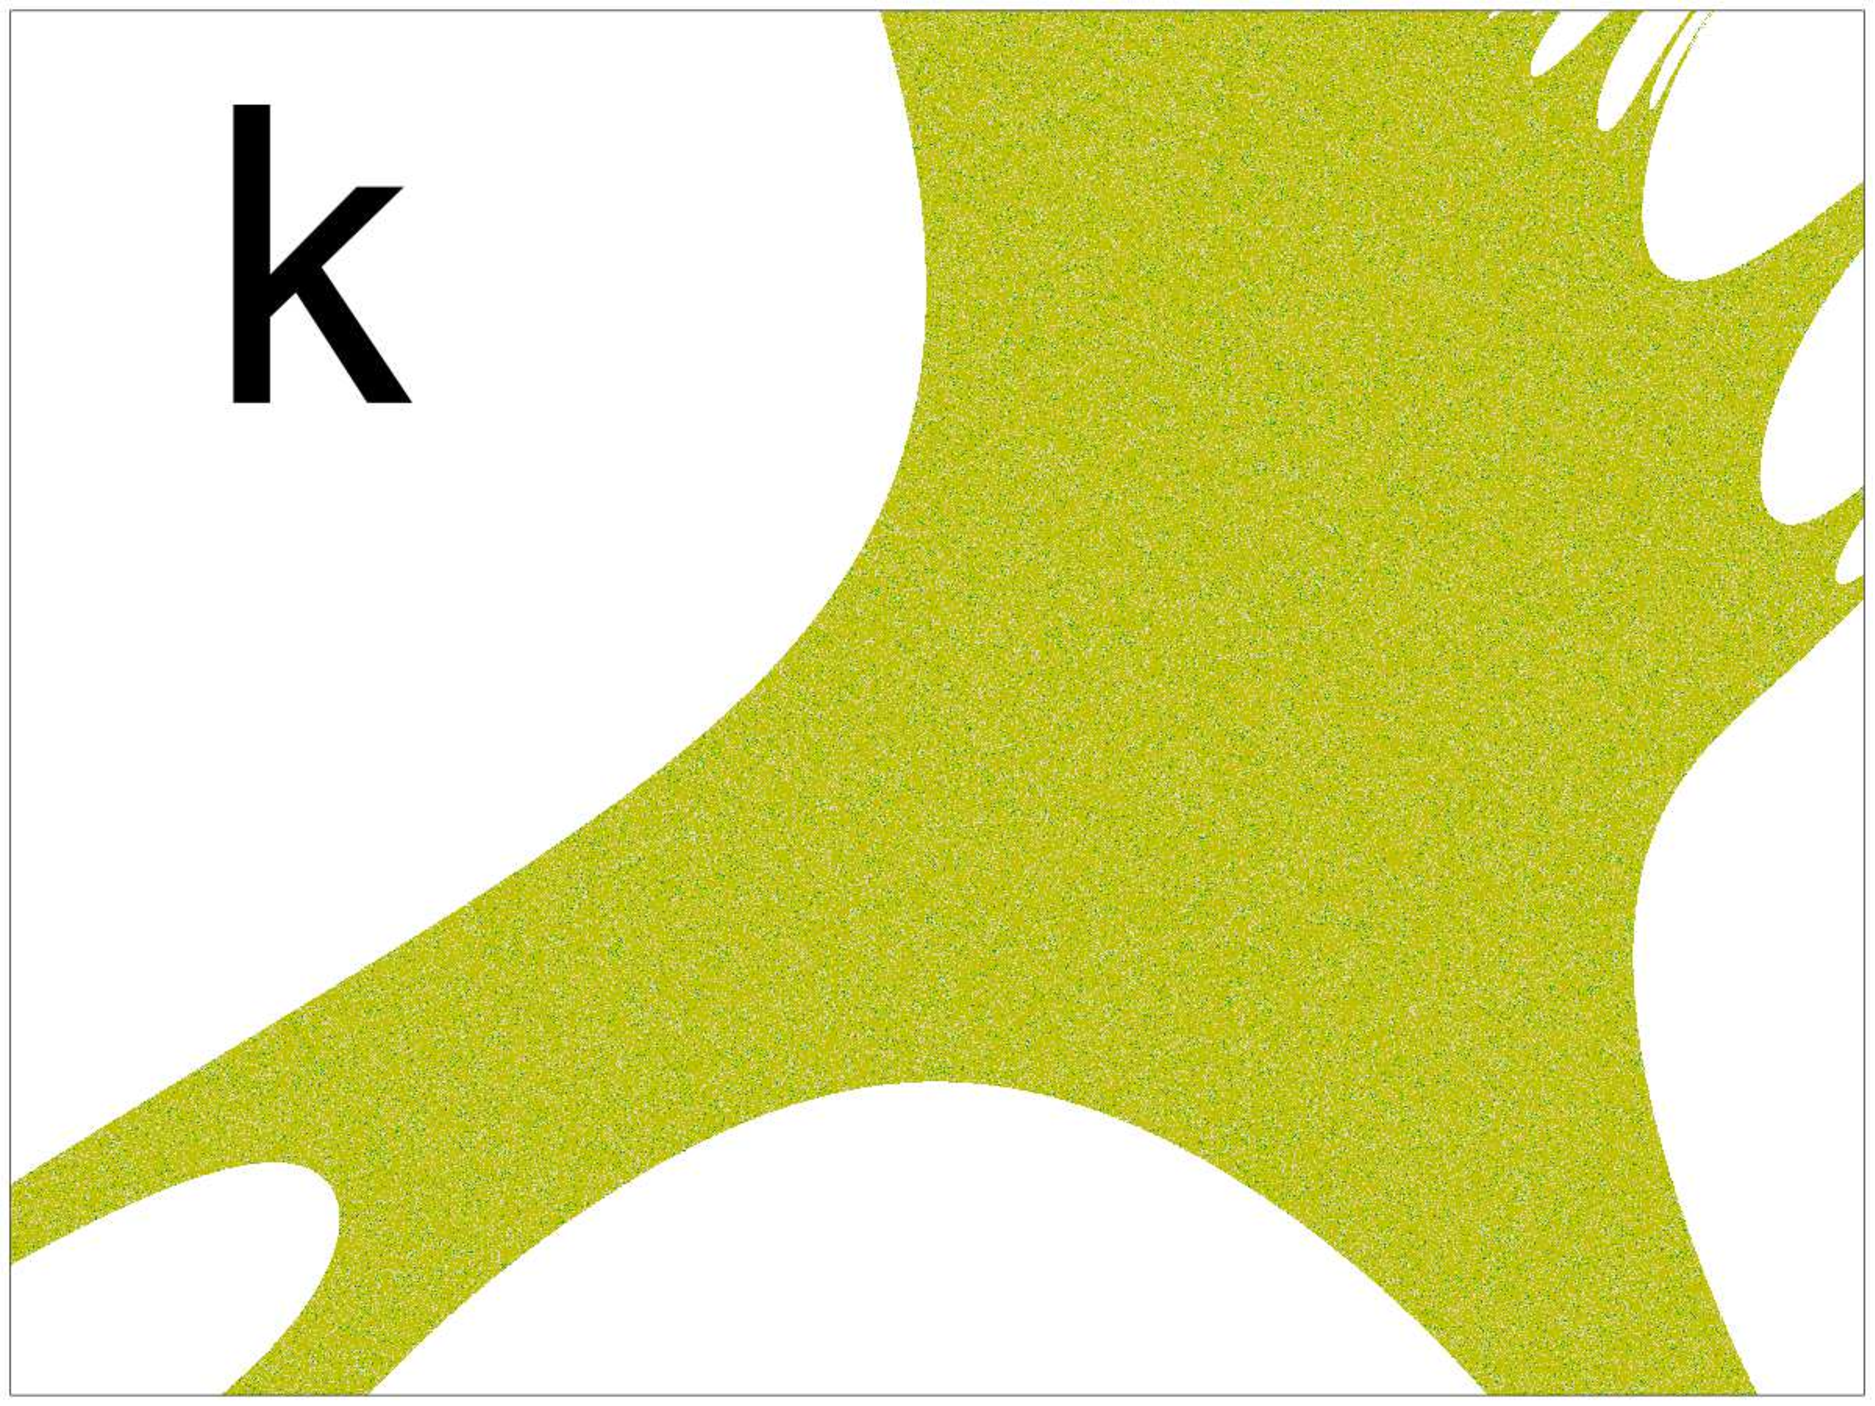
\includegraphics[width=0.35\textwidth]{m17}
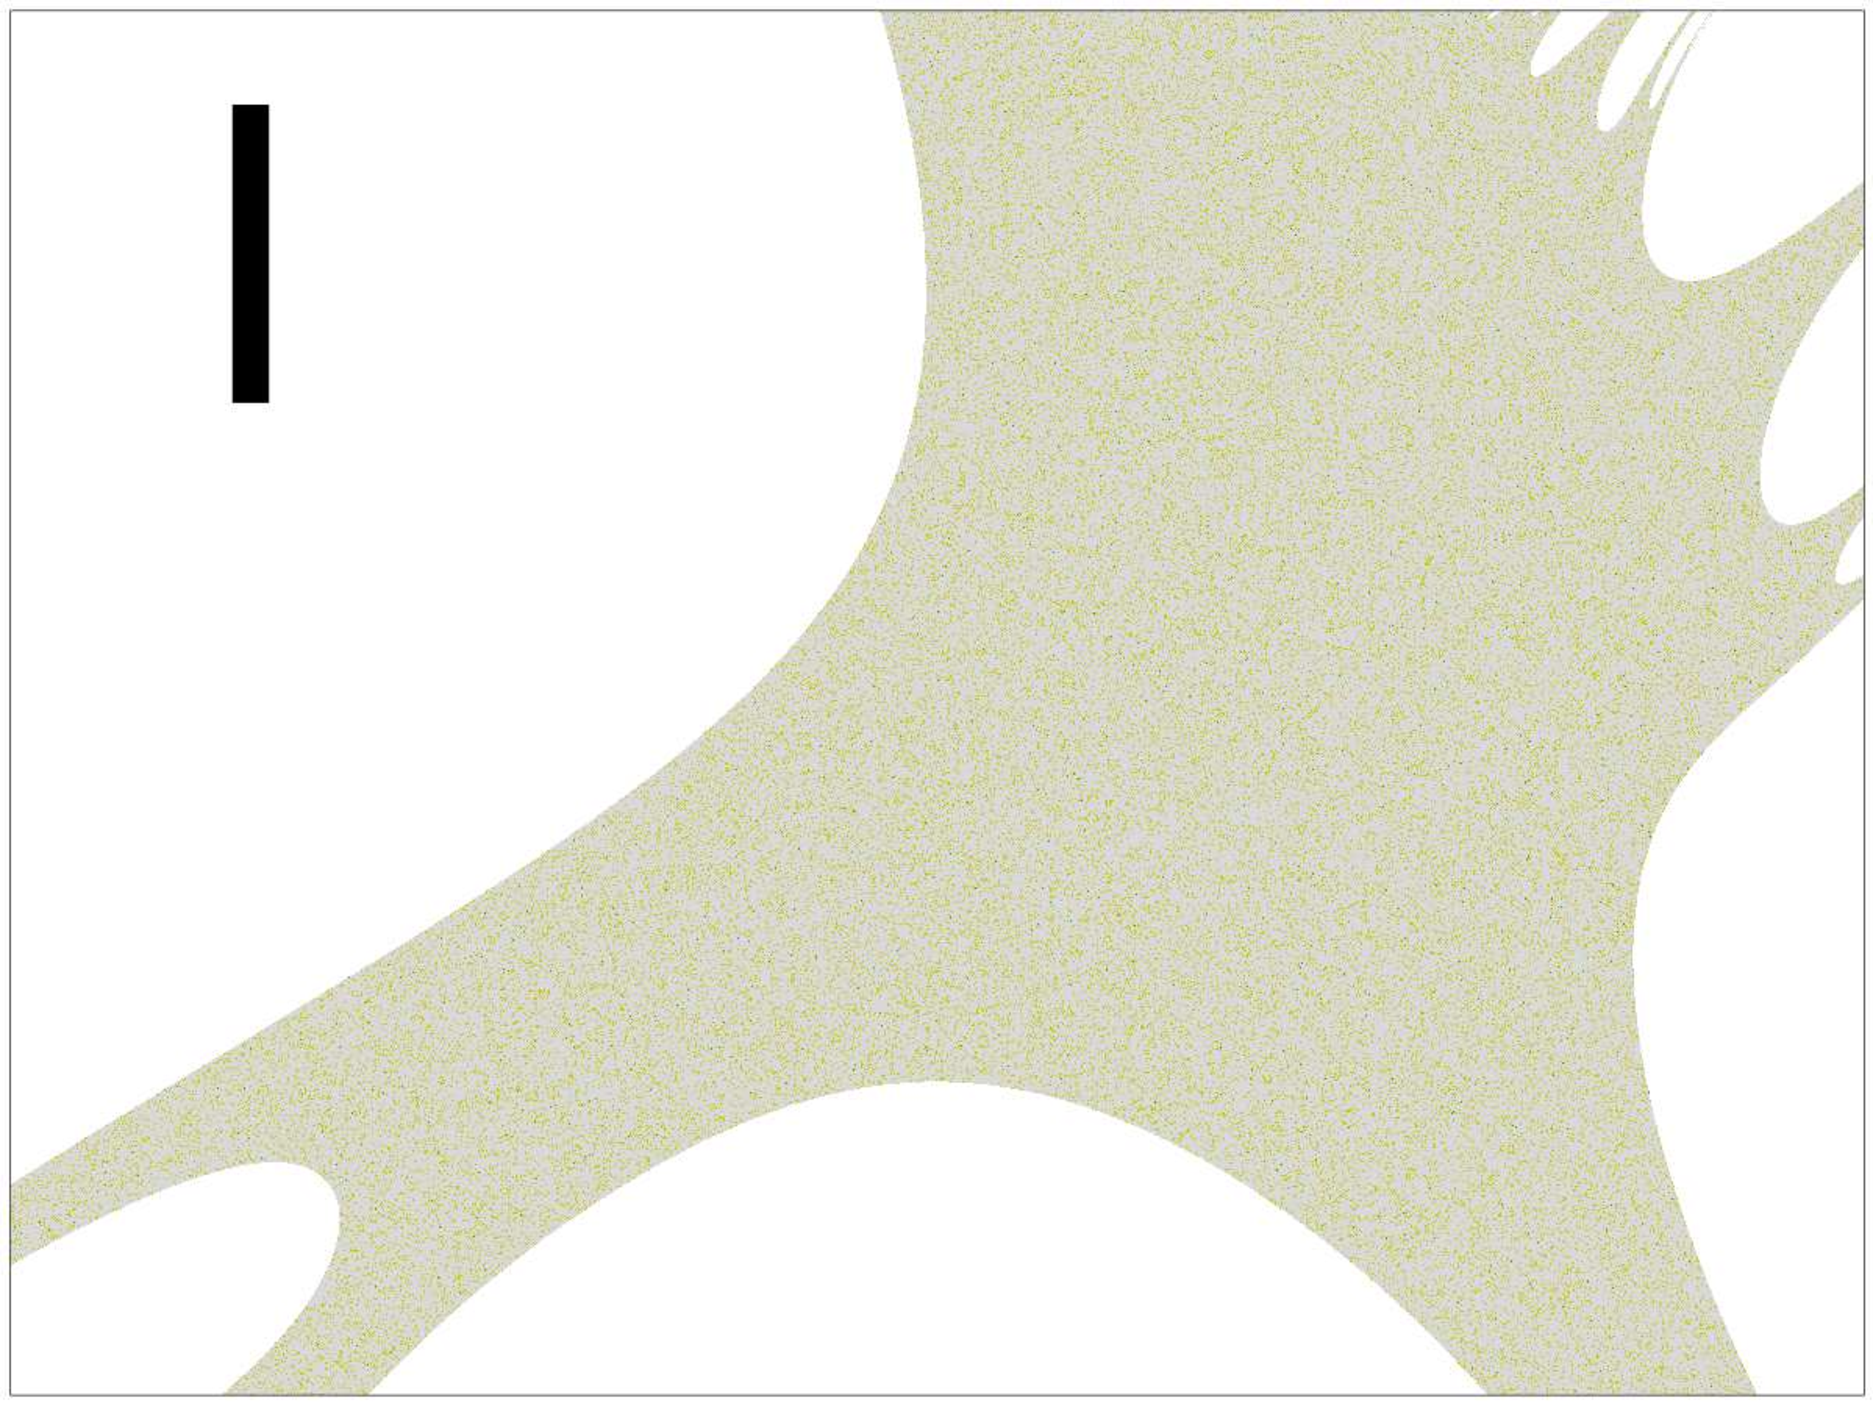
\includegraphics[width=0.35\textwidth]{m18}\\
\\   
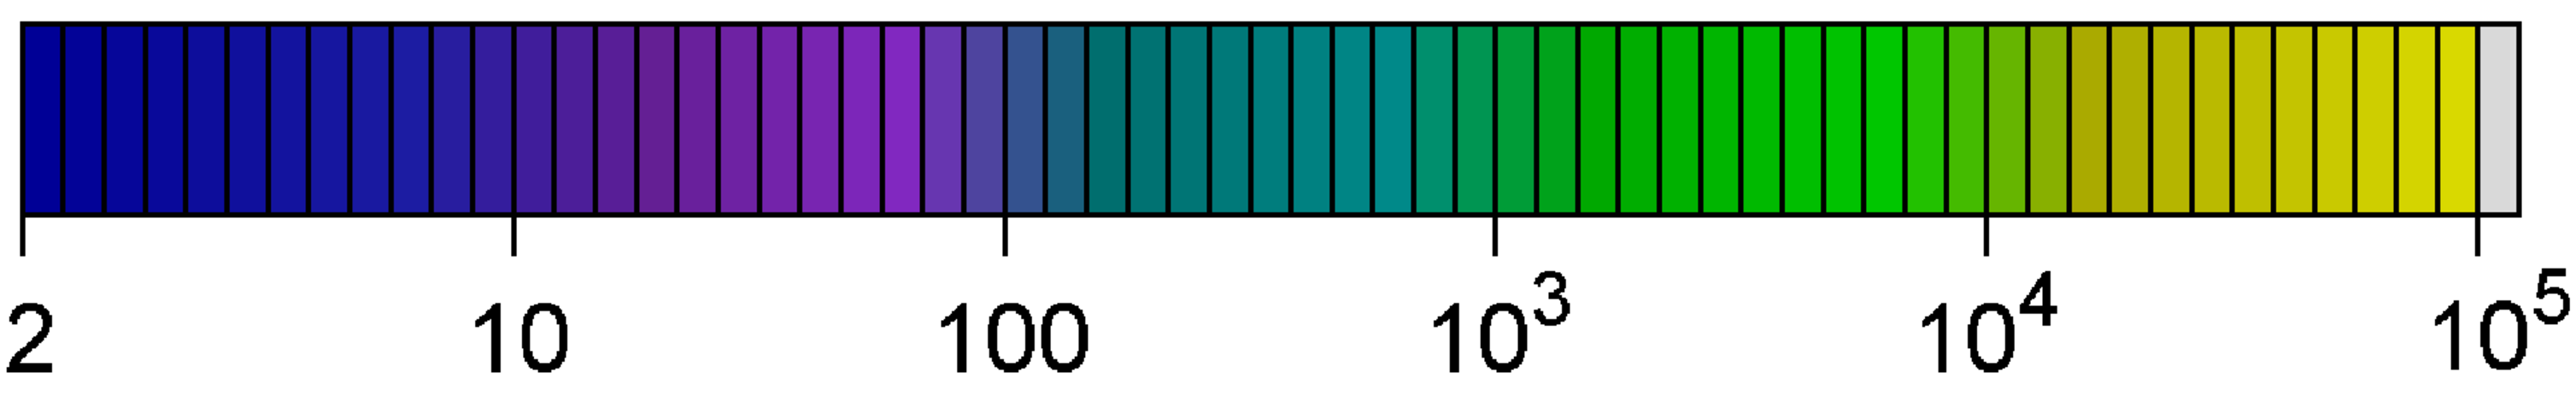
\includegraphics[width=0.6\textwidth]{ColorMapConEje}
\end{tabular}
\caption{Evolución de las longitudes de período de los dominios de atracción para: (a) $n_f=5$, (b) $n_f=6$, (c) $n_f=7$, (d) $n_f=8$, (e) $n_f=9$, (f) $n_f=10$, (g) $n_f=11$, (h) $n_f=12$, (i) $n_f=13$, (j) $n_f=14$, (k) $n_f=17$, (l) $n_f=18$.}
\label{fig:m}
\end{figure*}

La figura \ref{fig:m} muestra que a medida que aumenta el valor de $n_f$ el color del área se vuelve más uniforme y claro, lo que indica que las ICs convergen a ciclos de períodos más altos.
Esto también se puede ver en la tabla \ref{tabla}, donde a medida que $n_f$ aumenta, la longitud del ciclo límite predominante también aumenta.

Para comparar los valores obtenidos con las secuencias reales, iteramos los atractores en punto flotante con mantisa de $236$ bits (IEEE754 de punto flotante binario de precisión de octuple) lo que llamamos aquí \textit{punto flotante} o simplemente \textit{flotante}, es la aritmética más cercana a los números reales a la que podemos acceder con tiempos de cómputo razonables.
Luego, utilizando esa precisión en flotantes, todos los ciclos límite son superiores a $10 ^ 5$, convergen al atractor caótico que se ve en la figura \ref{fig:atractores3592}.d.

\begin{table*}[!t]
% increase table row spacing, adjust to taste
\renewcommand{\arraystretch}{1.3}
\caption{Lengths of the periods within the attractor domain $x$ and $y$ $\epsilon$  $[-2,2]$.}
\label{tabla}
\centering
\fontsize{9}{9}\selectfont
\begin{tabular}{l  l  }
	\hline
	$n_f$   & $T$ {\scriptsize(Percentage of ICs that converge to this period's length cycle)}                                                                                                                                           \\ \hline\hline
	$5$     & $2$ {\scriptsize($92.7\%$ )};$6$  {\scriptsize($7.3\% )$}                                                                                                                                                                  \\
	$6$     & $88$ {\scriptsize($41.6 \% )$};$44$ {\scriptsize($36.7 \% )$};$12$ {\scriptsize($13.8\% )$};$16$ {\scriptsize($6.2 \% )$};$2$ {\scriptsize($0.8 \% )$};$24$ {\scriptsize($0.6 \% )$};$26$ {\scriptsize($0.2 \%)$}          \\
	$7$     & $12$ {\scriptsize($83.5 \% )$};$14$ {\scriptsize($8.9\% )$};$24$ {\scriptsize($5.2\% )$};$34$ {\scriptsize($1.8 \% )$};$2$ {\scriptsize($0.6\% )$}                                                                         \\
	$8$     & $68$ {\scriptsize($91.7\%)$};$14$ {\scriptsize($6.2\%)$};$12$ {\scriptsize($1.8 \%)$};$17$ {\scriptsize($0.2\% )$};$15$ {\scriptsize($0.1 \%)$}                                                                            \\
	$9$     & $140$ {\scriptsize($54.5 \%)$};$123$ {\scriptsize($25.4 \%)$};$34$ {\scriptsize($8.6\%)$};$44$ {\scriptsize($4.3 \%)$};$38$ {\scriptsize($3.9 \%)$};$22$ {\scriptsize($2.9 \%)$};$48$;$2$;$12$;$4$ {\scriptsize($<0.1\%)$} \\
	$10$    & $655$ {\scriptsize($78.2\%)$};$212$ {\scriptsize($21.1\%)$};$143$ {\scriptsize($0.5\%)$};$12$ {\scriptsize($0.1\%)$};$2$;$36$;$13$;$20$;$10$;$4$ {\scriptsize($<0.1\%)$}                                                   \\
	$11$    & $153$ {\scriptsize($78.1\%)$};$461$ {\scriptsize($10.8\% )$};$1381$ {\scriptsize($8.7\%)$};$434$ {\scriptsize($2.3\%)$};$18$;$30$;$53$;$32$;$34$;$10$;$2$ {\scriptsize($<0.1\% )$}                                         \\
	$12$    & $2,278$ {\scriptsize($64.4\%)$};$438$ {\scriptsize($22.4\% )$};$598$ {\scriptsize($7.6\% )$};$886$ {\scriptsize($4.7 \%)$};$12$ {\scriptsize($0.7\%)$};$87$;$2$;$42$;$23$;$32$;$10$ {\scriptsize($<0.1\% )$}               \\
	$13$    & $11,510$ {\scriptsize($ 98.9\%)$};$1052$ {\scriptsize($1 \%)$};$12$;$26$;$2$;$10$ {\scriptsize($<0.1\% )$}                                                                                                                 \\
	$14$    & $21,333$ {\scriptsize($69.2\% )$};$5.804$ {\scriptsize($16.5\%  )$};$4,795$ {\scriptsize($7.9\%  )$};$1,264$ {\scriptsize($5.8 \% )$};$2,429$ {\scriptsize($0.5\% )$}                                                      \\
	        & $46$;$23$;$21$;$10$;$12$;$17$ {\scriptsize($<0.1\%  )$}                                                                                                                                                                    \\
	$15$    & $10,099$ {\scriptsize($58.6 \%)$};$1.762$ {\scriptsize($19.4 \%)$};$14,887$ {\scriptsize($18.3\%)$};$1,598$ {\scriptsize($3.4\%)$};$750$;$105$;$23$;$14$;$2$;$10$ {\scriptsize($<0.1\%)$}                                  \\
	$16$    & $54,718$ {\scriptsize($87.5\% )$};$5,017$ {\scriptsize($4.7\% )$};$>10^5$ {\scriptsize($3.7\% )$};$5,367$ {\scriptsize($2.5\% )$};$703$ {\scriptsize($0.9\% )$}                                                            \\
	        & $1,159$;$1,802$ {\scriptsize($0.2\% )$};$377$;$75$;$10$ {\scriptsize($<0.1\%  )$}                                                                                                                                          \\
	$17$    & $37,812$ {\scriptsize($53.1\% )$};$38,456$ {\scriptsize($24.1\% )$};$>10^5$ {\scriptsize($16.0\%)$};$34,749$ {\scriptsize($3.0\% )$};$3,362$;$718$ {\scriptsize($1.5\%)$}                                                  \\
	        & $3,006$,$5,222$ {\scriptsize($0.1\% )$};$15$ {\scriptsize($<0.1 \%)$}                                                                                                                                                      \\
	$18$    & $>10^5$ {\scriptsize($87.4\%)$};$52,069$ {\scriptsize($12.5\% )$};$2,471$ {\scriptsize($0.1\% )$};$146$;$51$ {\scriptsize($<0.1 \%)$}                                                                                      \\
	$float$ & $>10^5$ {\scriptsize($100\% )$}                                                                                                                                                                                            \\ \hline
\end{tabular}

\end{table*}

En relación con los cuantificadores de la aleatoriedad, nos dimos cuenta de que el análisis realizado hasta este punto no era suficiente para describir completamente los cambios en la dinámica de un sistema caótico digitalizado.
Alcanzar períodos largos no garantiza que los sistemas exhiban buenas propiedades con respecto a la aleatoriedad.
Así que decidimos estudiar más a fondo los datos obtenidos mediante el empleo de cuantificadores estadísticos.

Como se dijo, en la Fig. \ref{fig:avvelo}.a las dos zonas grises corresponden a las condiciones iniciales que convergen a los dos ciclos coexistentes de período dos y seis, respectivamente.
Entonces, estos dos ciclos tendrán un valor determinado de  $H_{BP}$, $H_{hist}\mid_{T=2}=0.0625$, $H_{hist}\mid_{T=6}=0.1199$, $H_{BP}\mid_{T=2}=0.1053$ y $H_{BP} \mid_{T = 6} = 0.2723 $.
Sin embargo, el valor reportado de estos cuantificadores no puede ser el promedio de ambos, ya que la tasa de ocurrencia del ciclo dos es mucho mayor que la del ciclo seis (el período dos aparece $92.7 \%$ veces mientras que el período seis solo $7.3 \%$, ver Tabla \ref{tabla}).
Por lo tanto, hemos calculado los cuantificadores promedios ponderando cada cuantificador por su tasa de ocurrencia.
%
\begin{figure}
    \centering
        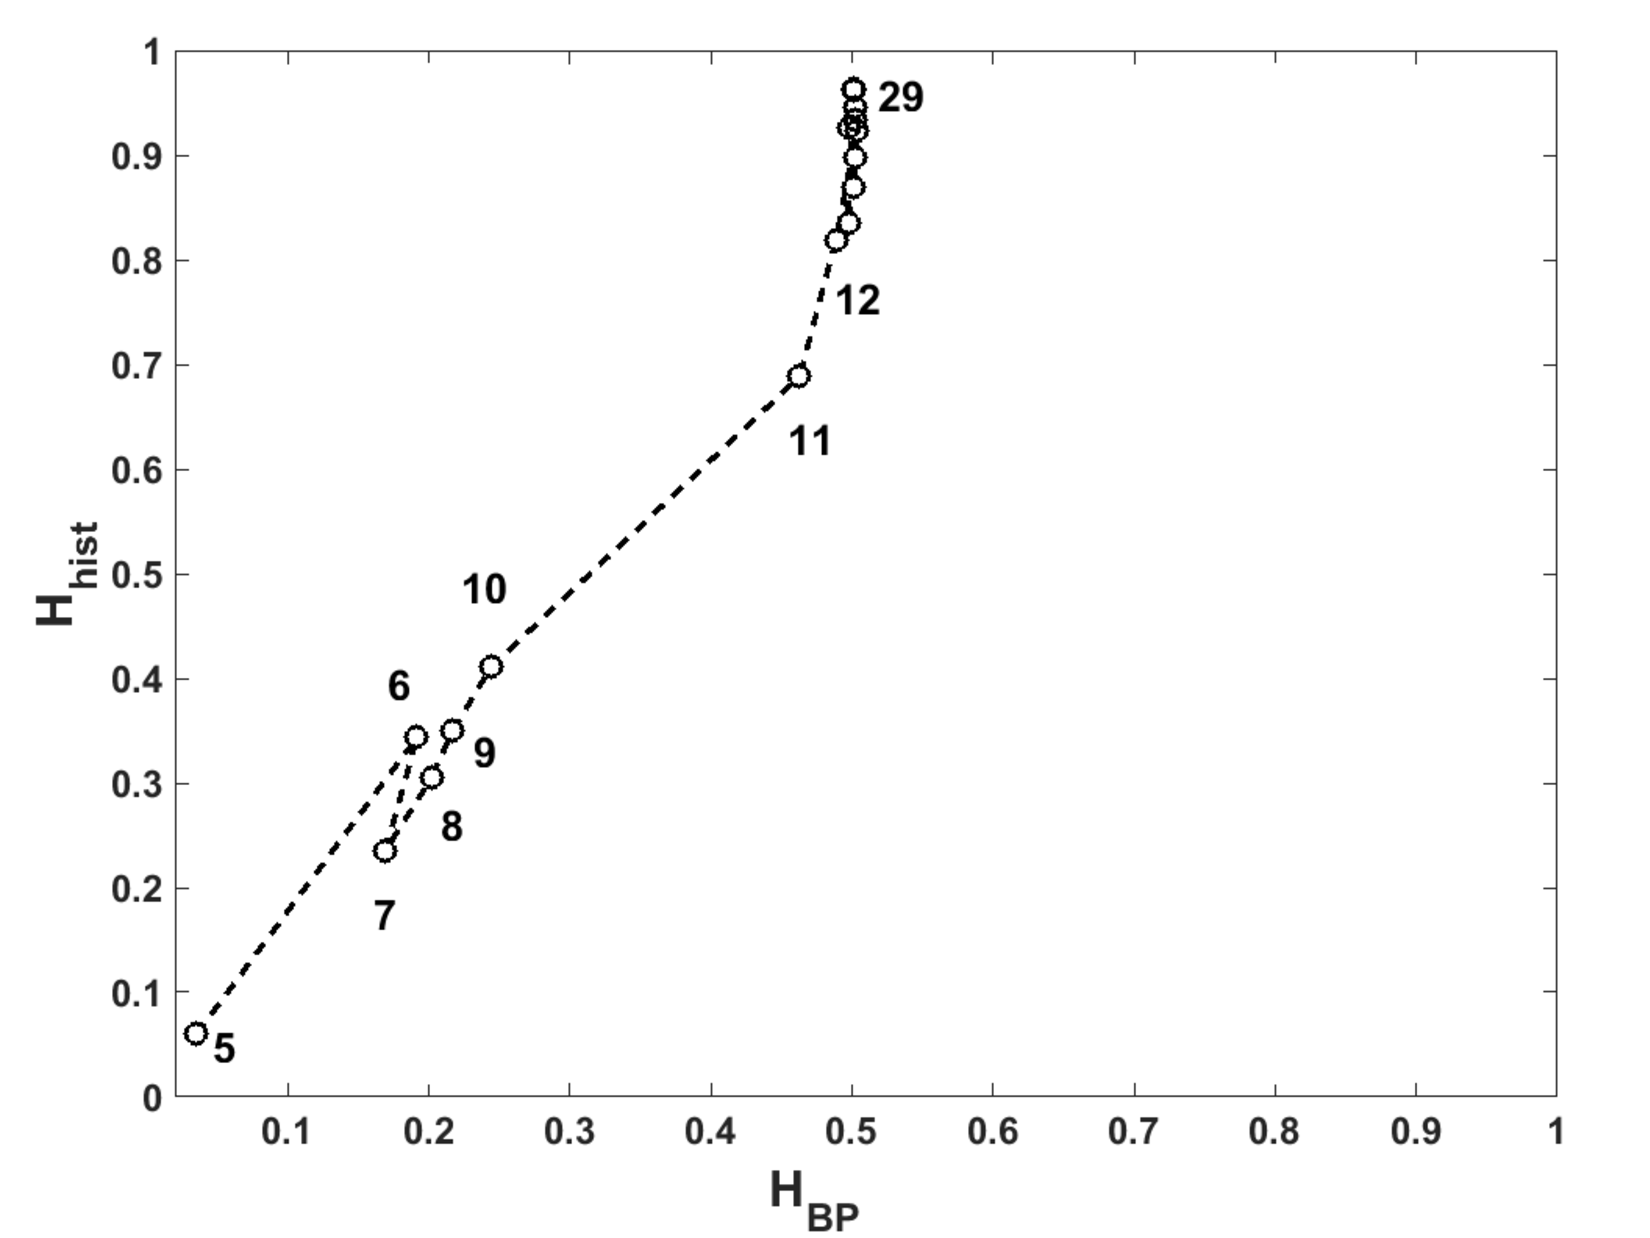
\includegraphics[width=0.85\columnwidth]{HBPvsHhistO}\\
    \caption{Plano $H_{hist}$ - $H_{BP}$ para diferentes números de bits. }\label{fig:HBPvsHhist}
\end{figure}

El plano $H_{hist}$ vs $H_{BP}$, que se muestra en la Fig. \ref{fig:HBPvsHhist}, permite una visualización rápida del comportamiento en términos de aleatoriedad del sistema, en este plano el punto ``ideal", desde el punto de vista estadístico, es $(1,1)$.
Aquí, el sistema parece estabilizarse para $n_f$ superior a $12$.
Se puede observar que mientras $H_{hist}$ se estabiliza cerca del valor máximo ($ H_{hist} = 1 $), el $H_{BP}$ tiende a estabilizarse a $0.5$.
Este valor de $ H_{BP} $ es característico de los sistemas caóticos y se debe a las estructuras internas de sus atractores.

Un resumen del análisis observado de estos resultados se puede ver en la Fig. \ref{puntos}.
%
\begin{figure}
    \centering
    \begin{subfigure}[b]{0.49\textwidth}
        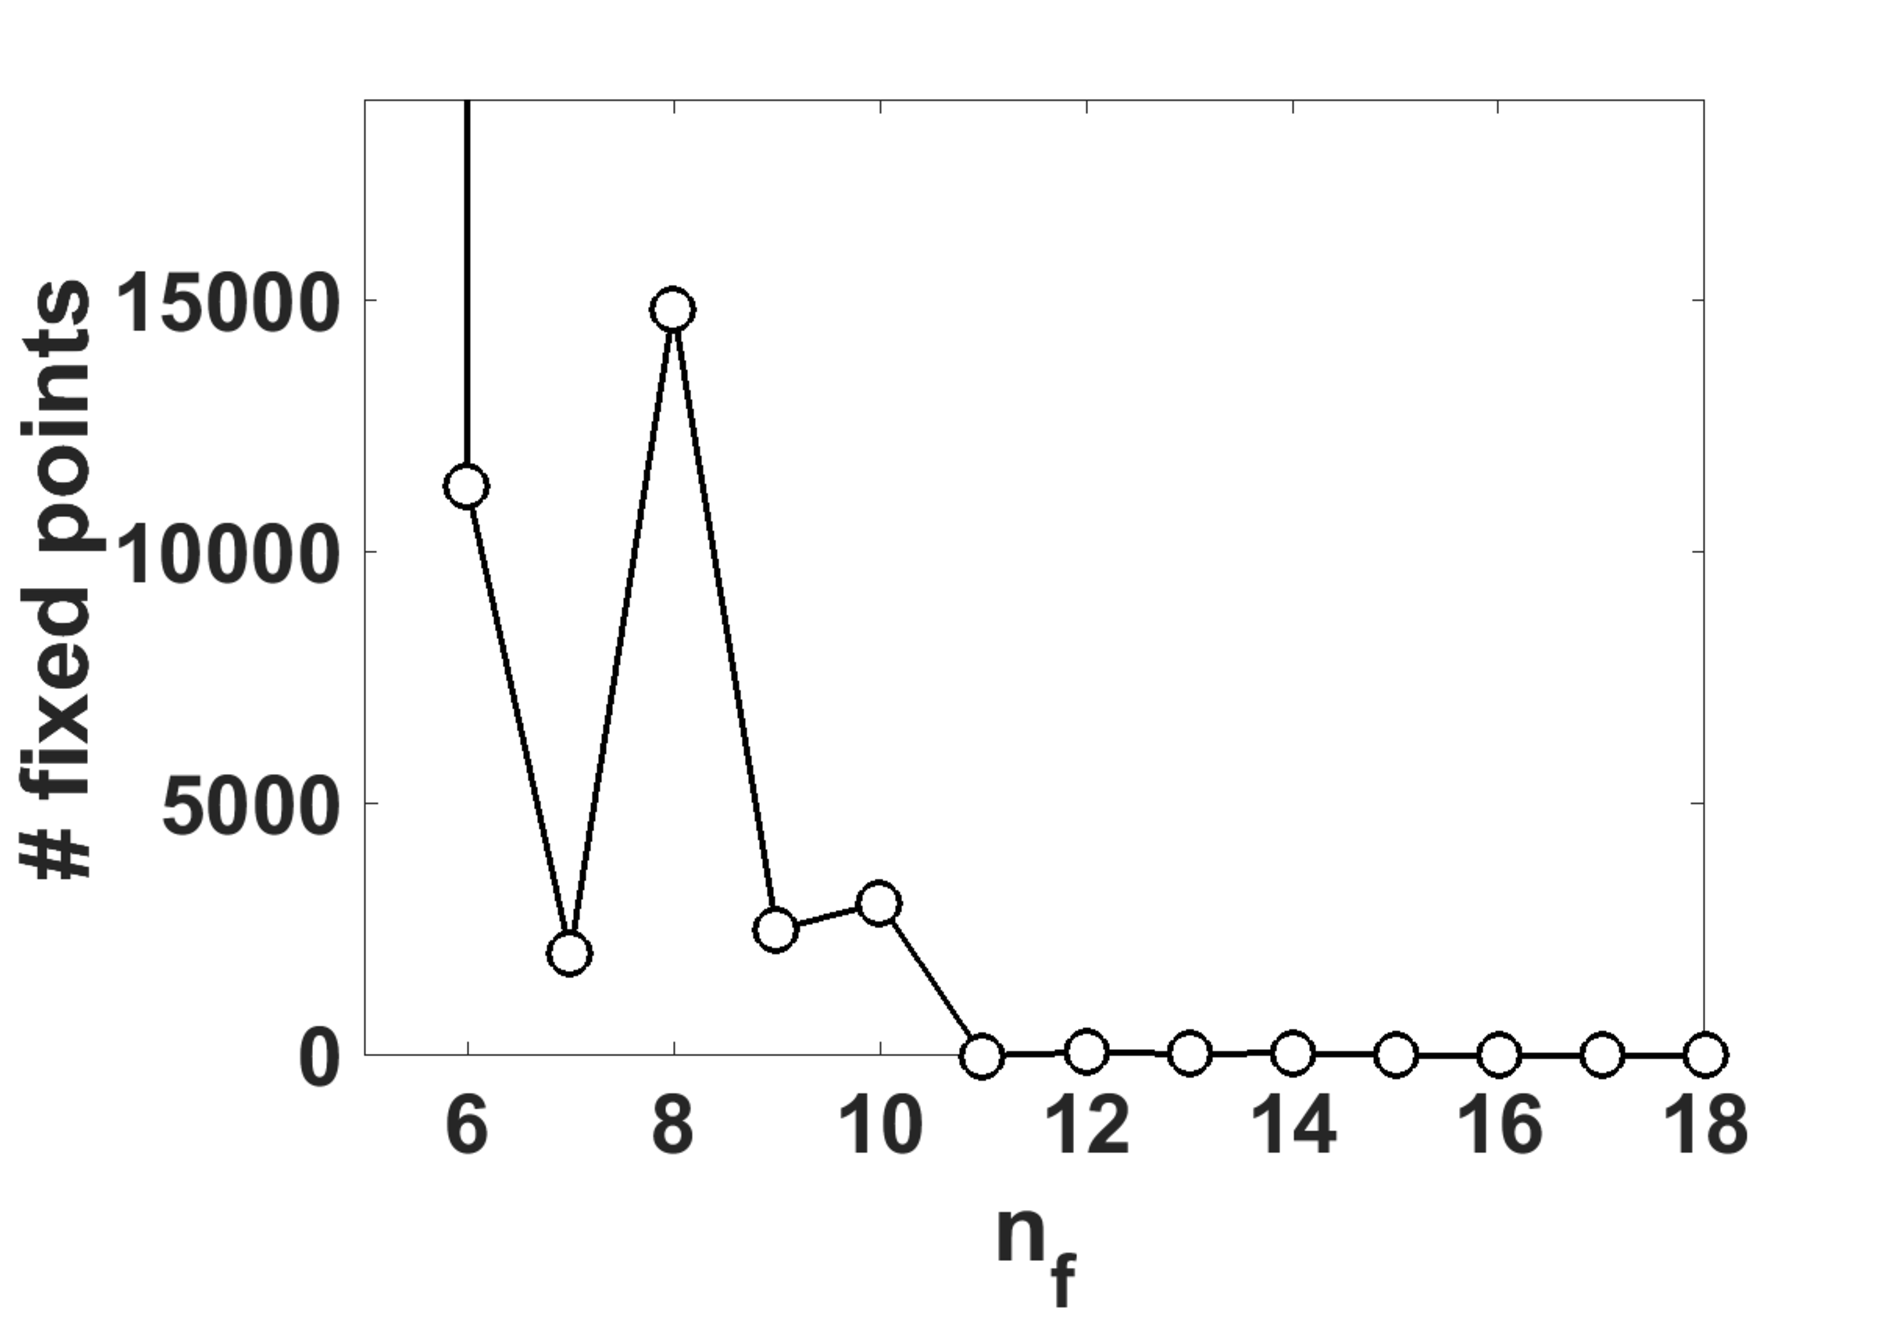
\includegraphics[width=\textwidth]{ptosfijosO}
        \caption{number of fixed points.}
        \label{fig:gull}
    \end{subfigure}
    \hfill 
    \begin{subfigure}[b]{0.49\textwidth}
        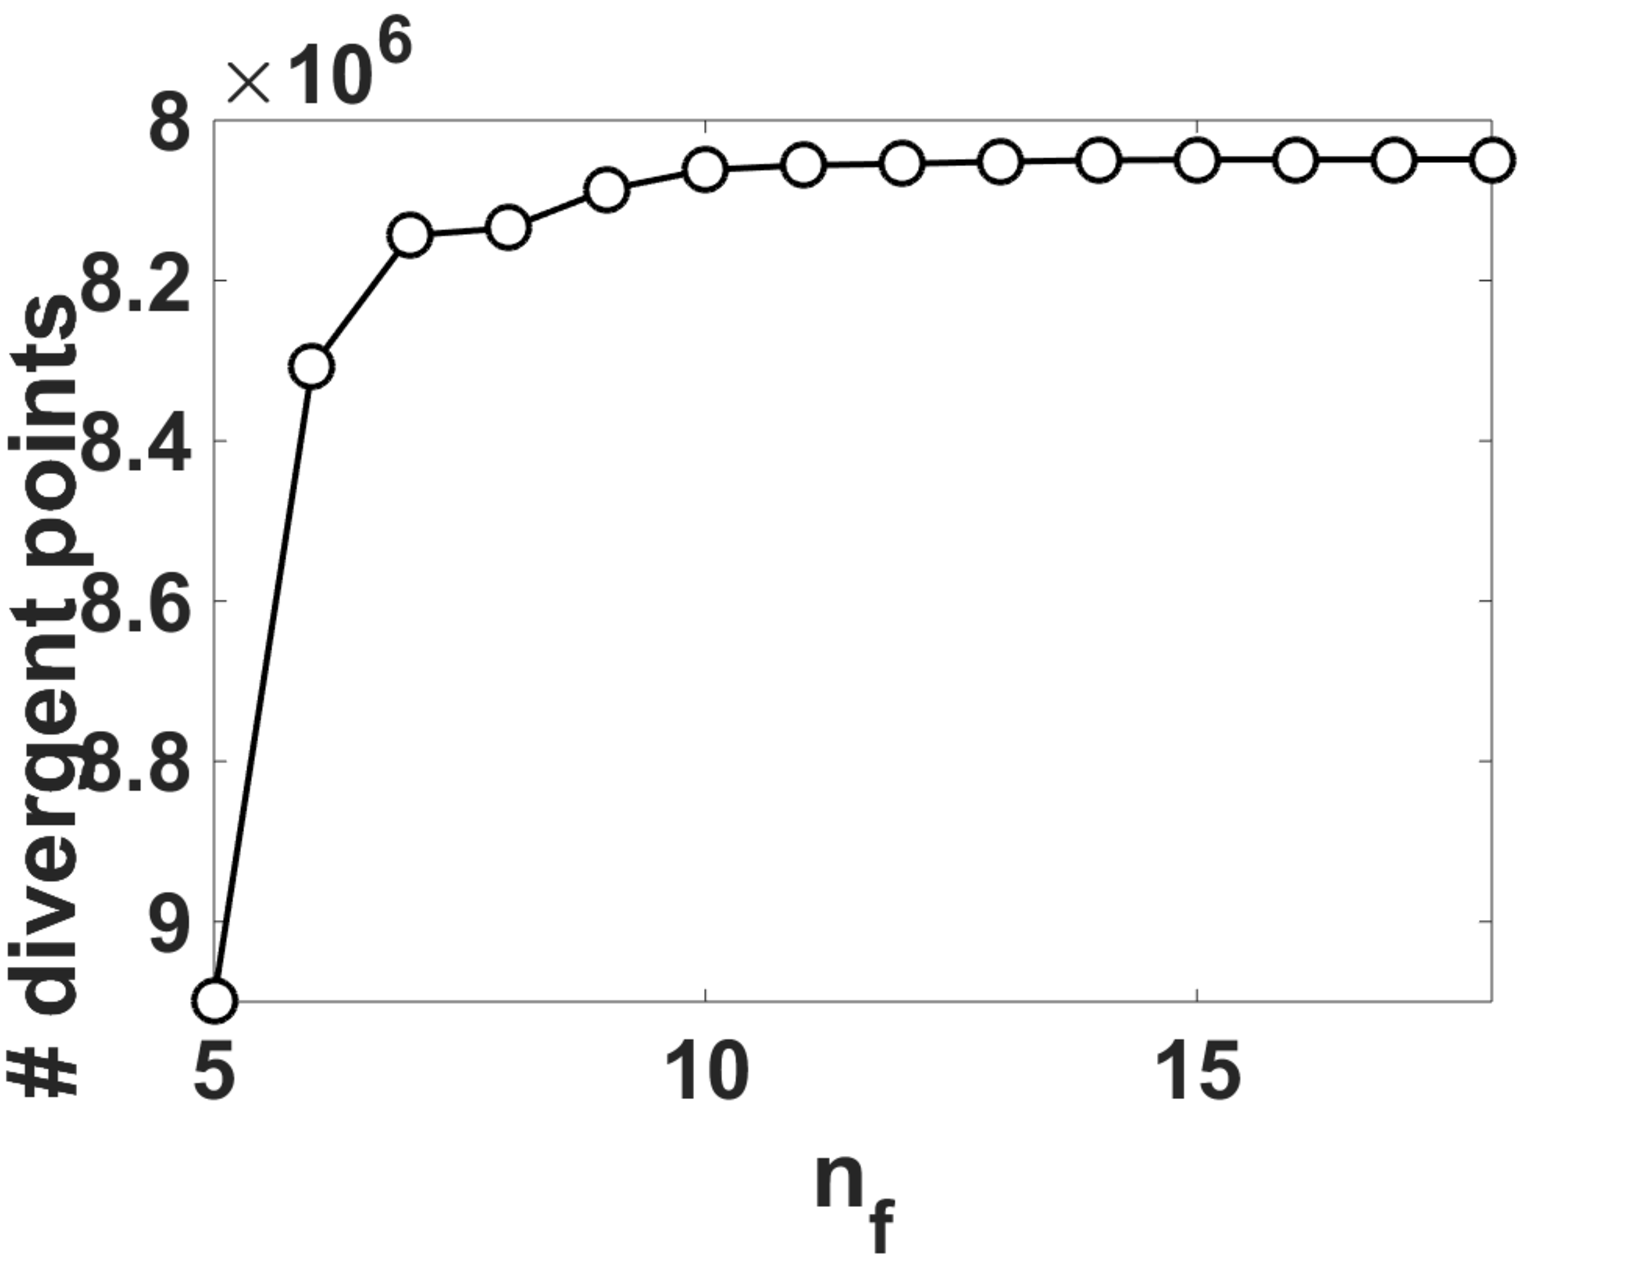
\includegraphics[width=\textwidth]{divergenO}
        \caption{number of divergent points.}
        \label{fig:tiger}
    \end{subfigure}
   \hfill 
    \begin{subfigure}[b]{0.49\textwidth}
        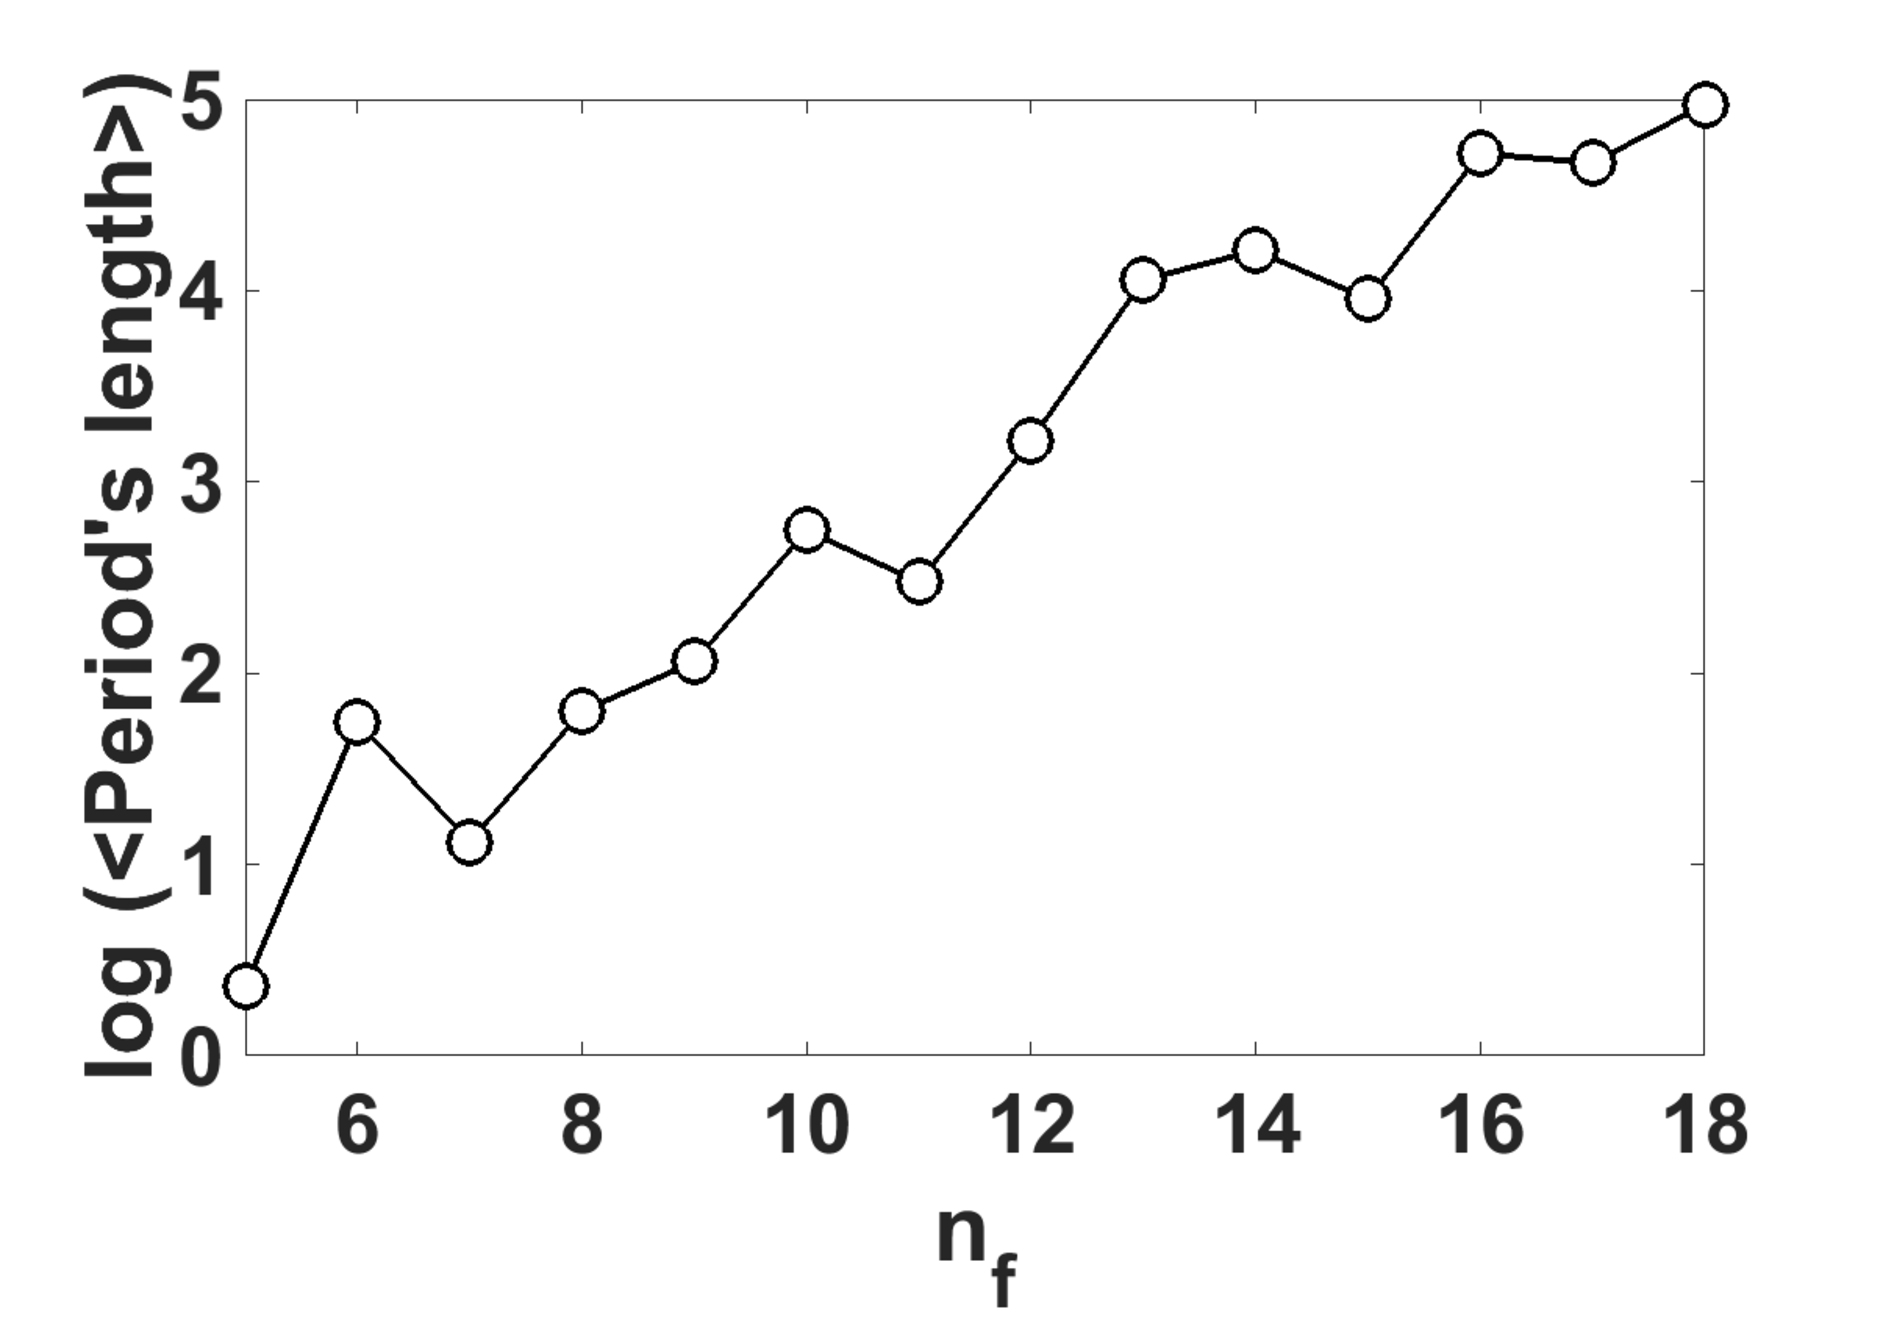
\includegraphics[width=\textwidth]{Periodos_promO}
        \caption{logarithm of the length's cycles weighted average.}
        \label{fig:mouse}
    \end{subfigure}
  \hfill   
    \begin{subfigure}[b]{0.49\textwidth}
        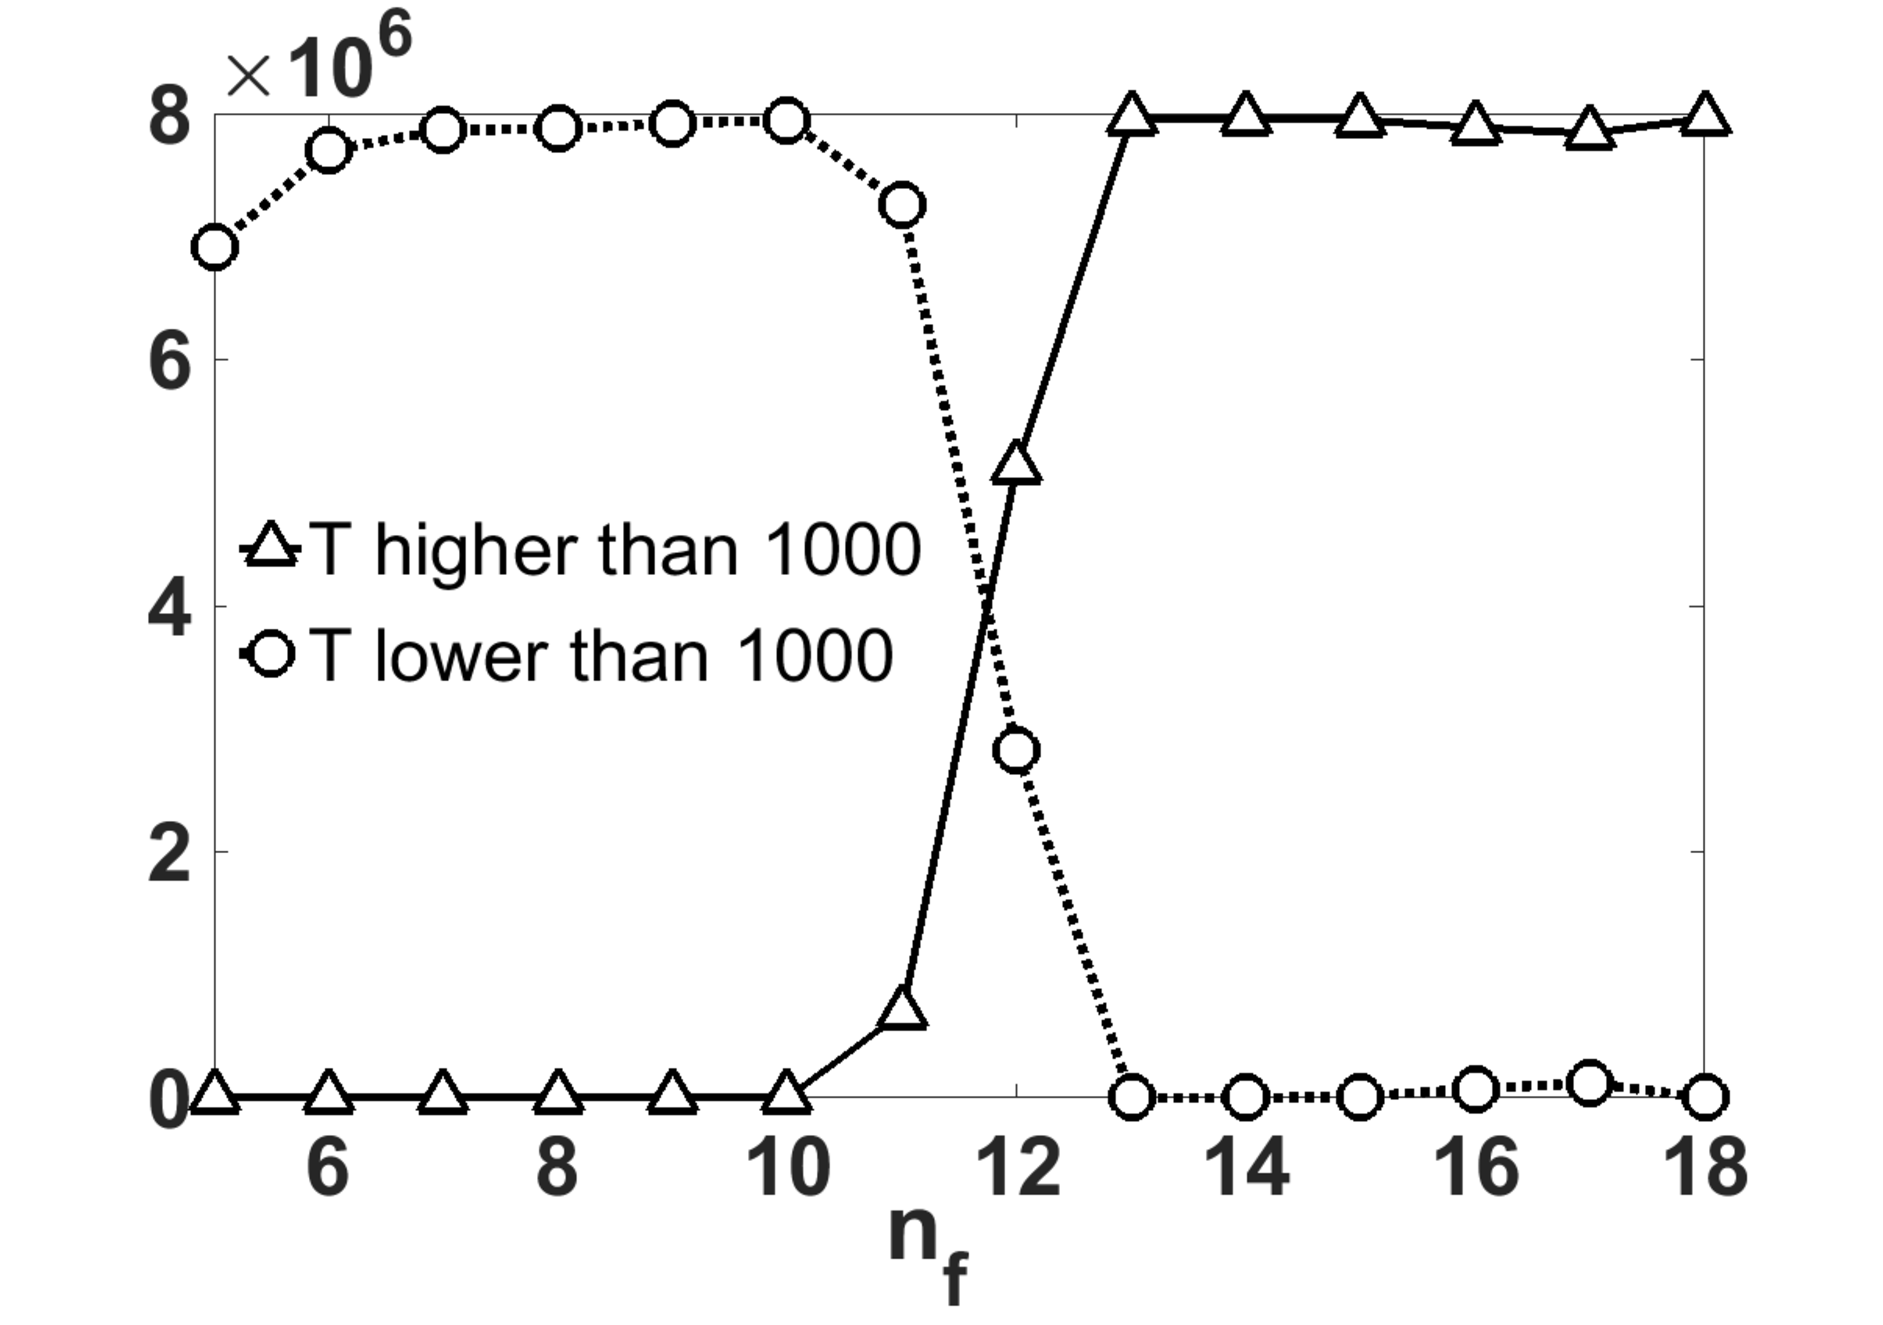
\includegraphics[width=\textwidth]{PuntosO}
        \caption{initial conditions with period length higher and lower than $1,000$.}
        \label{fig:mouse}
    \end{subfigure}
    \caption{Summary of initial conditions' behavior.}\label{puntos}
\end{figure}
%
La Fig. \ref{puntos}.a y \ref{puntos}.b muestran el número de puntos que divergen y convergen en puntos fijos respectivamente a medida que aumenta el valor de $n_f$, en ambos casos, el valor final tiende al que se obtiene en implementación en punto flotante.
De estas figuras se desprende que para $n_f \sim 12$ el sistema parece haberse estabilizado.
La figura \ref{puntos}.c muestra que el período promediado aumenta a una velocidad logarítmica.
Finalmente, la Fig. \ref{puntos}.d muestra el número de condiciones iniciales que presentan períodos $T$ más altos y más bajos que $1,000$.
De nuevo, un valor de $12$ para $n_f$ parece ser el límite para obtener una buena aproximación del sistema.

La figura \ref{fig:HBPHhist} muestra el promedio ponderado de los cuantificadores $H_{hist}$, $H_{BP}$ y \textsl{MLE}.
En la figura se puede ver que los tres cuantificadores tienden al valor calculado usando aritmética de punto flotante.
Mientras $H_{BP}$ y \textsl{MLE} se estabilizan para $n_f \sim 12$ o $13$, $H_{hist}$ alcanza el valor en coma flotante de $n_f \sim 19$, mostrando que hay propiedades de las secuencias de salida que solo este cuantificador puede detectar.
Esto confirma la necesidad de usar ambos cuantificadores para caracterizar la aleatoriedad de las secuencias.
%
\begin{figure}
    \centering
        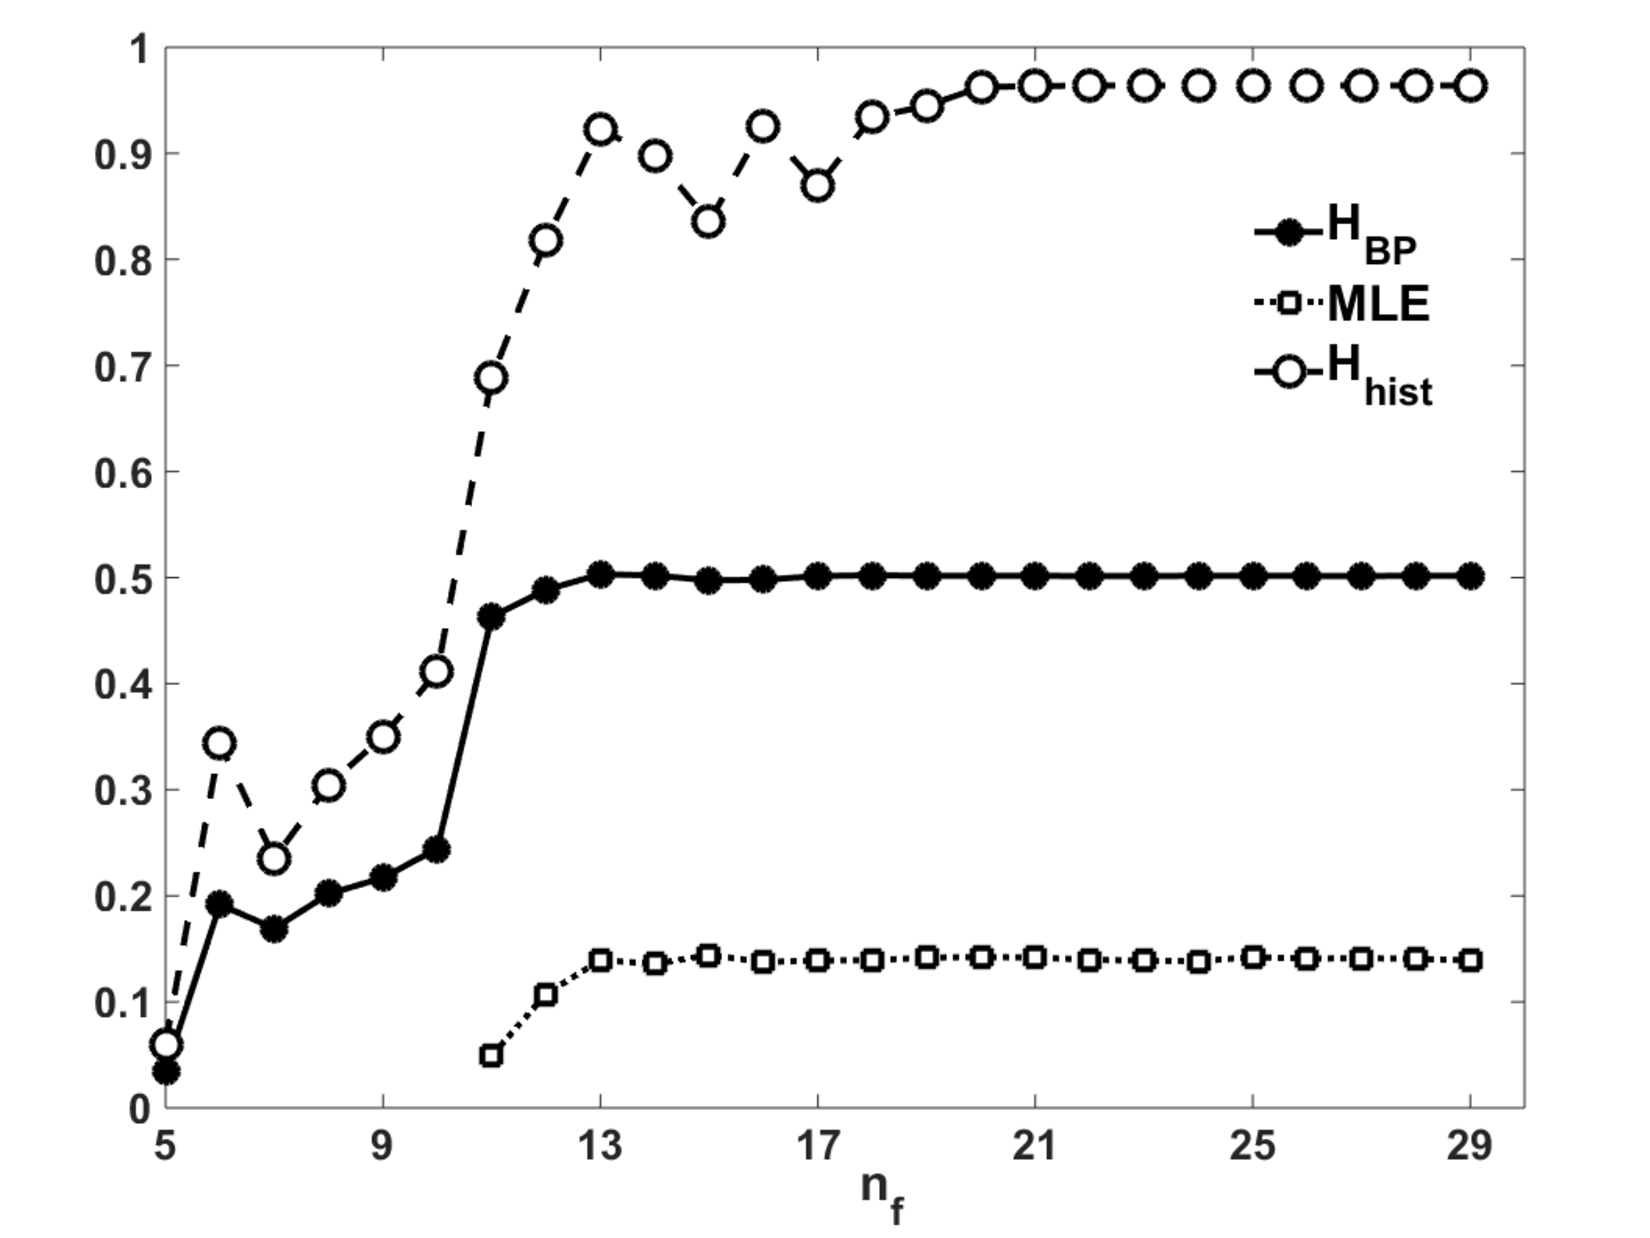
\includegraphics[width=0.75\columnwidth]{HBPHhistO}\\
    \caption{Weighted average of quantifiers $H_{BP}$,  $H_{hist}$ and \textsl{MLE} as functions of the number of bits.}\label{fig:HBPHhist}
\end{figure}
%
Como puede verse en el análisis anterior, el número mínimo de bits está determinado por $H_{hist}$ y los resultados son $n_f = 19$ más la cantidad de bits utilizados para representar la parte entera $n_i = 4$, por lo tanto $n_{min}$ resulta ser igual a $23$.
